\chapter{Analisi dei risultati delle simulazioni}
\label{ch:results_analysis}
\section{Introduzione}
\label{sec:intro_results_analysis}
In questo capitolo vengono presentati i risultati delle simulazioni condotte con il simulatore Virtuoso Cadence \textcopyright. In particolare, si analizzeranno i risultati ottenuti per i quattro scenari di test definiti nel capitolo \ref{chap:Nauta_Miller_Comparison}.

Il primo passo per l'analisi dei risultati è la creazione di uno schematico di riferimento per la simulazione. Nelle prossime sezioni verranno mostrati gli schematici di riferimento per ciascuno dei quattro scenari di test, insieme ai risultati delle simulazioni. Gli schematici di riferimento sono stati progettati in modo da essere comparabili, strutturandoli in modo gerarchico. Verranno presentati i blocchi più esterni, che rappresentano l'OTA come amplificatore operazionale, e i blocchi interni, che rappresentano le singole configurazioni circuitali fino ad arrivare al transistor.

\section{Analisi dei risultati per l'OTA di Nauta a stadio singolo}
\label{sec:results_ota_nauta_single_stage}


\subsubsection{Schematico di riferimento per la simulazione}
\label{sec:results_ota_nauta_single_stage_reference_schematic}
Lo schematico rappresenta un OTA di Nauta a stadio singolo con una capacità di carico di 1pF. La figura \ref{fig:schematic_nauta_single_stage} mostra lo schematico di riferimento utilizzato per le simulazioni.

\begin{figure}[H]
    \centering
    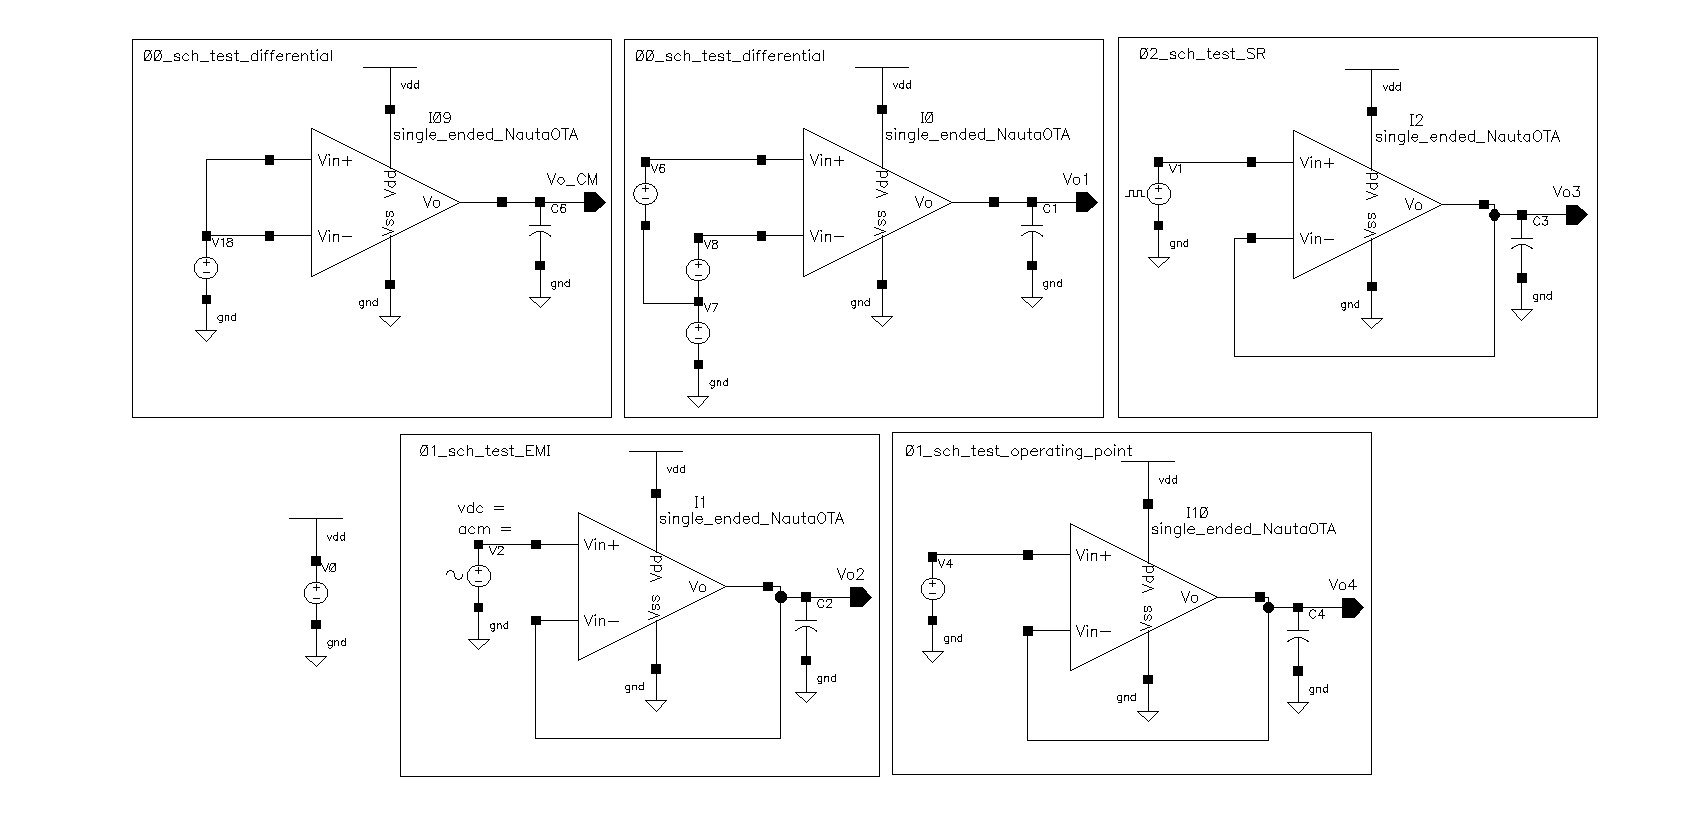
\includegraphics[width=\textwidth]{img/nauta/single/sim_nauta_single_stage.png}
    \caption{Schematico di riferimento per l'OTA di Nauta a stadio singolo.}
    \label{fig:schematic_nauta_single_stage}
\end{figure}

Internamente, ogni cella \textit{single\_ended\_Nauta\_OTA} è composta da una serie di inverter collegati in cascata, come mostrato nella figura \ref{fig:schematic_nauta_single_stage_inverter}. Ogni inverter è composto da un transistor NMOS e un transistor PMOS, con i rispettivi valori di larghezza ($W_{NMOS}$ e $W_{PMOS}$) e lunghezza ($L_{NMOS}$ e $L_{PMOS}$) riportati nella Tabella \ref{tab:component_sizing_nauta_single_stage}.

\begin{figure}[H]
    \centering
    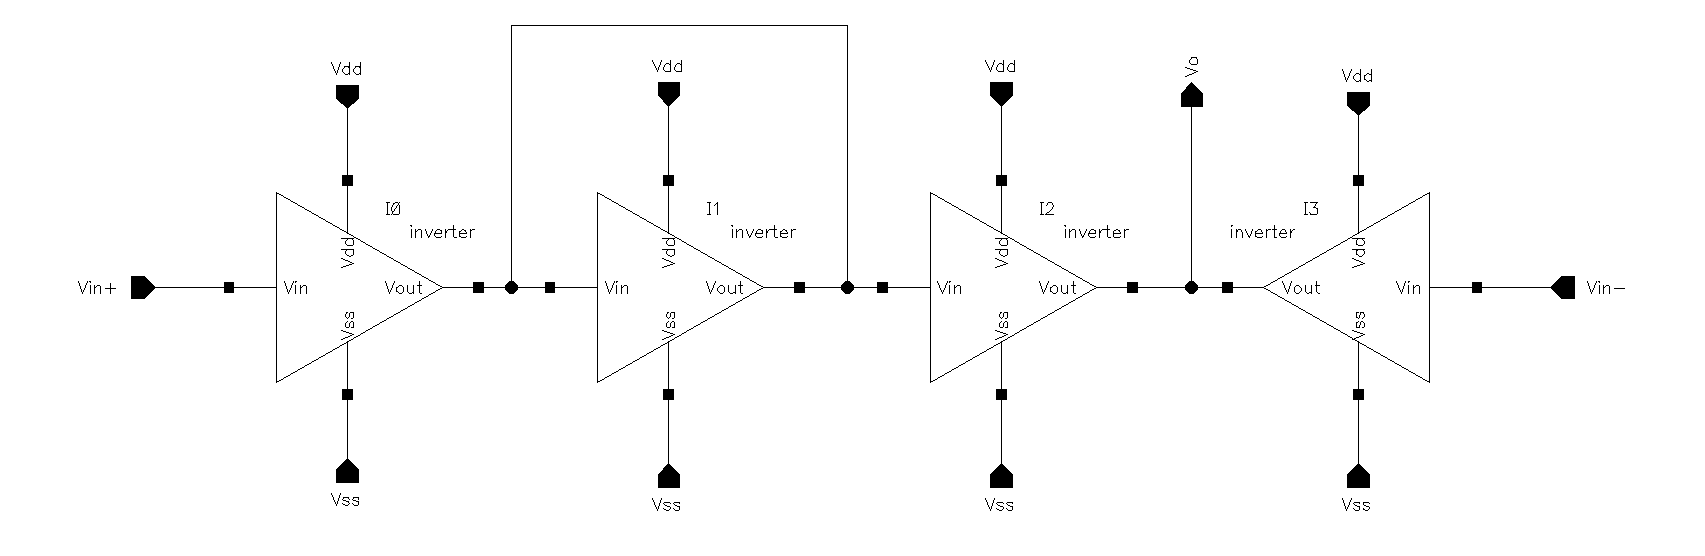
\includegraphics[width=\textwidth]{img/nauta/single/sch_nauta_single_stage.png}
    \caption{Schematico di riferimento per l'inverter dell'OTA di Nauta a stadio singolo.}
    \label{fig:schematic_nauta_single_stage_inverter}
\end{figure}

Di seguito, viene mostrato lo schematico di riferimento per la cella inverter base, che è composta da un transistor NMOS e un transistor PMOS.

\begin{figure}[H]
    \centering
    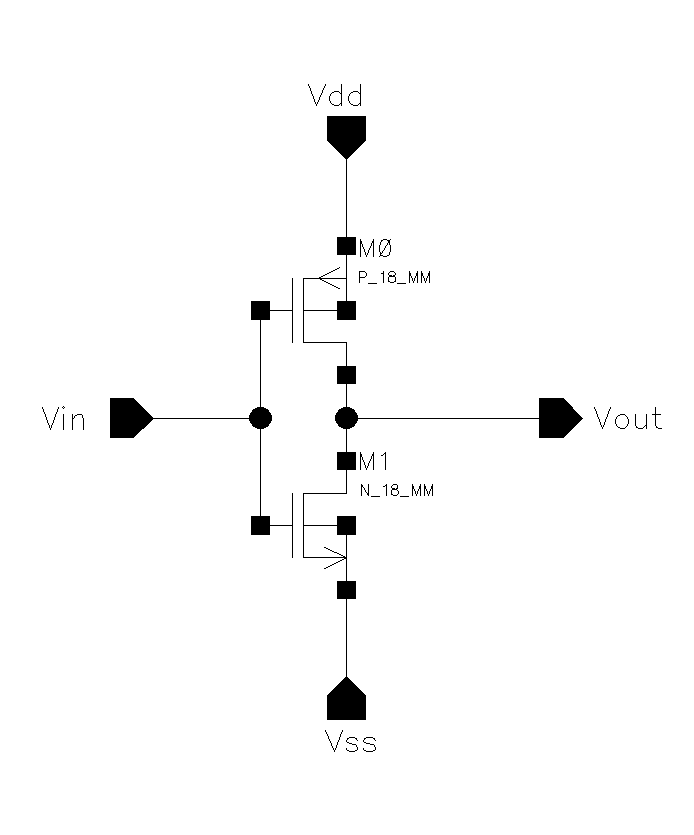
\includegraphics[width=0.5\textwidth]{img/nauta/single/sch_inverter.png}
    \caption{Schematico di riferimento per la cella inverter base.}
    \label{fig:schematic_inverter_base}
\end{figure}

\subsubsection{Dimensionamento dei componenti}
\label{sec:results_ota_nauta_single_stage_component_sizing}

I parametri di dimensionamento sono stati scelti in modo da garantire un guadagno di tensione intorno a 40 dB e un margine di fase di almeno 60°. I valori di dimensionamento scelti e i relativi risultati sono riportati nella Tabella \ref{tab:component_sizing_nauta_single_stage}.

Si può osservare che le regioni operative dei transistor per tensione di alimentazione superiore a 0.5V sono tutte nella regione di saturazione (regione 2), il che è un buon segno per il corretto funzionamento dell'OTA. Inoltre, il guadagno di tensione e il margine di fase sono entrambi superiori ai valori minimi richiesti. Tuttavia, si nota che  per tensione di alimentazione di 0.5V è indicata regione di debole inversione (regione 3) per tutti i transistor. Questo accade perché il simulatore non è in grado di distinguere tra la regione di debole inversione e la regione di saturazione. Dai risultati ottenuti, si può comunque dedurre che i transistor siano in regione di saturazione.

\begin{table}[H]
    \centering
    \begin{tabular}{c|c|c|c|}
        \cline{2-4}
        & \textbf{Valim = 0.5V} & \textbf{Valim = 1V} & \textbf{Valim = 1.8V} \\ \hline
        \multicolumn{4}{|c|}{\textbf{Parametri di simulazione}} \\ \hline
        \multicolumn{1}{|c|}{\textbf{$L_{NMOS}$}} & 1$\mu$m & 4$\mu$m & 4$\mu$m \\ \hline
        \multicolumn{1}{|c|}{\textbf{$W_{NMOS}$}} & 10$\mu$m & 48$\mu$m & 48$\mu$m \\ \hline
        \multicolumn{1}{|c|}{\textbf{$\#finger_{NMOS}$}} & 10 & 12 & 12 \\ \hline
        \multicolumn{1}{|c|}{\textbf{$L_{PMOS}$}} & 1$\mu$m & 4$\mu$m & 4$\mu$m \\ \hline
        \multicolumn{1}{|c|}{\textbf{$W_{PMOS}$}} & 70$\mu$m & 280$\mu$m & 280$\mu$m \\ \hline
        \multicolumn{1}{|c|}{\textbf{$\#finger_{PMOS}$}} & 10 & 28 & 28 \\ \hline
        \multicolumn{4}{|c|}{\textbf{Risultati della simulazione}} \\ \hline
        \multicolumn{1}{|c|}{I0/M0 region} & 3 & 2 & 2 \\ \hline
        \multicolumn{1}{|c|}{I0/M1 region} & 3 & 2 & 2 \\ \hline
        \multicolumn{1}{|c|}{I1/M0 region} & 3 & 2 & 2 \\ \hline
        \multicolumn{1}{|c|}{I1/M1 region} & 3 & 2 & 2 \\ \hline
        \multicolumn{1}{|c|}{I2/M0 region} & 3 & 2 & 2 \\ \hline
        \multicolumn{1}{|c|}{I2/M1 region} & 3 & 2 & 2 \\ \hline
        \multicolumn{1}{|c|}{I3/M0 region} & 3 & 2 & 2 \\ \hline
        \multicolumn{1}{|c|}{I3/M1 region} & 3 & 2 & 2 \\ \hline
        \multicolumn{1}{|c|}{$A_V(0)$} & 36.36 & 41.14 & 37.99 \\ \hline
        \multicolumn{1}{|c|}{f$_c$} & 4.28kHz & kHz &  kHz \\ \hline
        \multicolumn{1}{|c|}{f$_o$} & 261.5kHz & MHz &  MHz \\ \hline
    \end{tabular}
    \caption{Dimensionamento dei componenti dell'OTA di Nauta a stadio singolo. Tutti i risultati sono stati ottenuti con una capacità di carico di 1pF.}
    \label{tab:component_sizing_nauta_single_stage}
\end{table}

\newpage
\subsubsection{\textbf{$A_V$}, Phase, CMRR e CMR}
\label{sec:results_ota_nauta_single_stage_A_V_phase_CMRR_CMR}

Di seguito vengono riportati i risultati delle simulazioni per il guadagno di tensione ($A_V$), la fase (Phase), il rapporto di reiezione al modo comume (CMRR) e il range di modo comune (CMR). 

\begin{figure}[H]
    \centering
    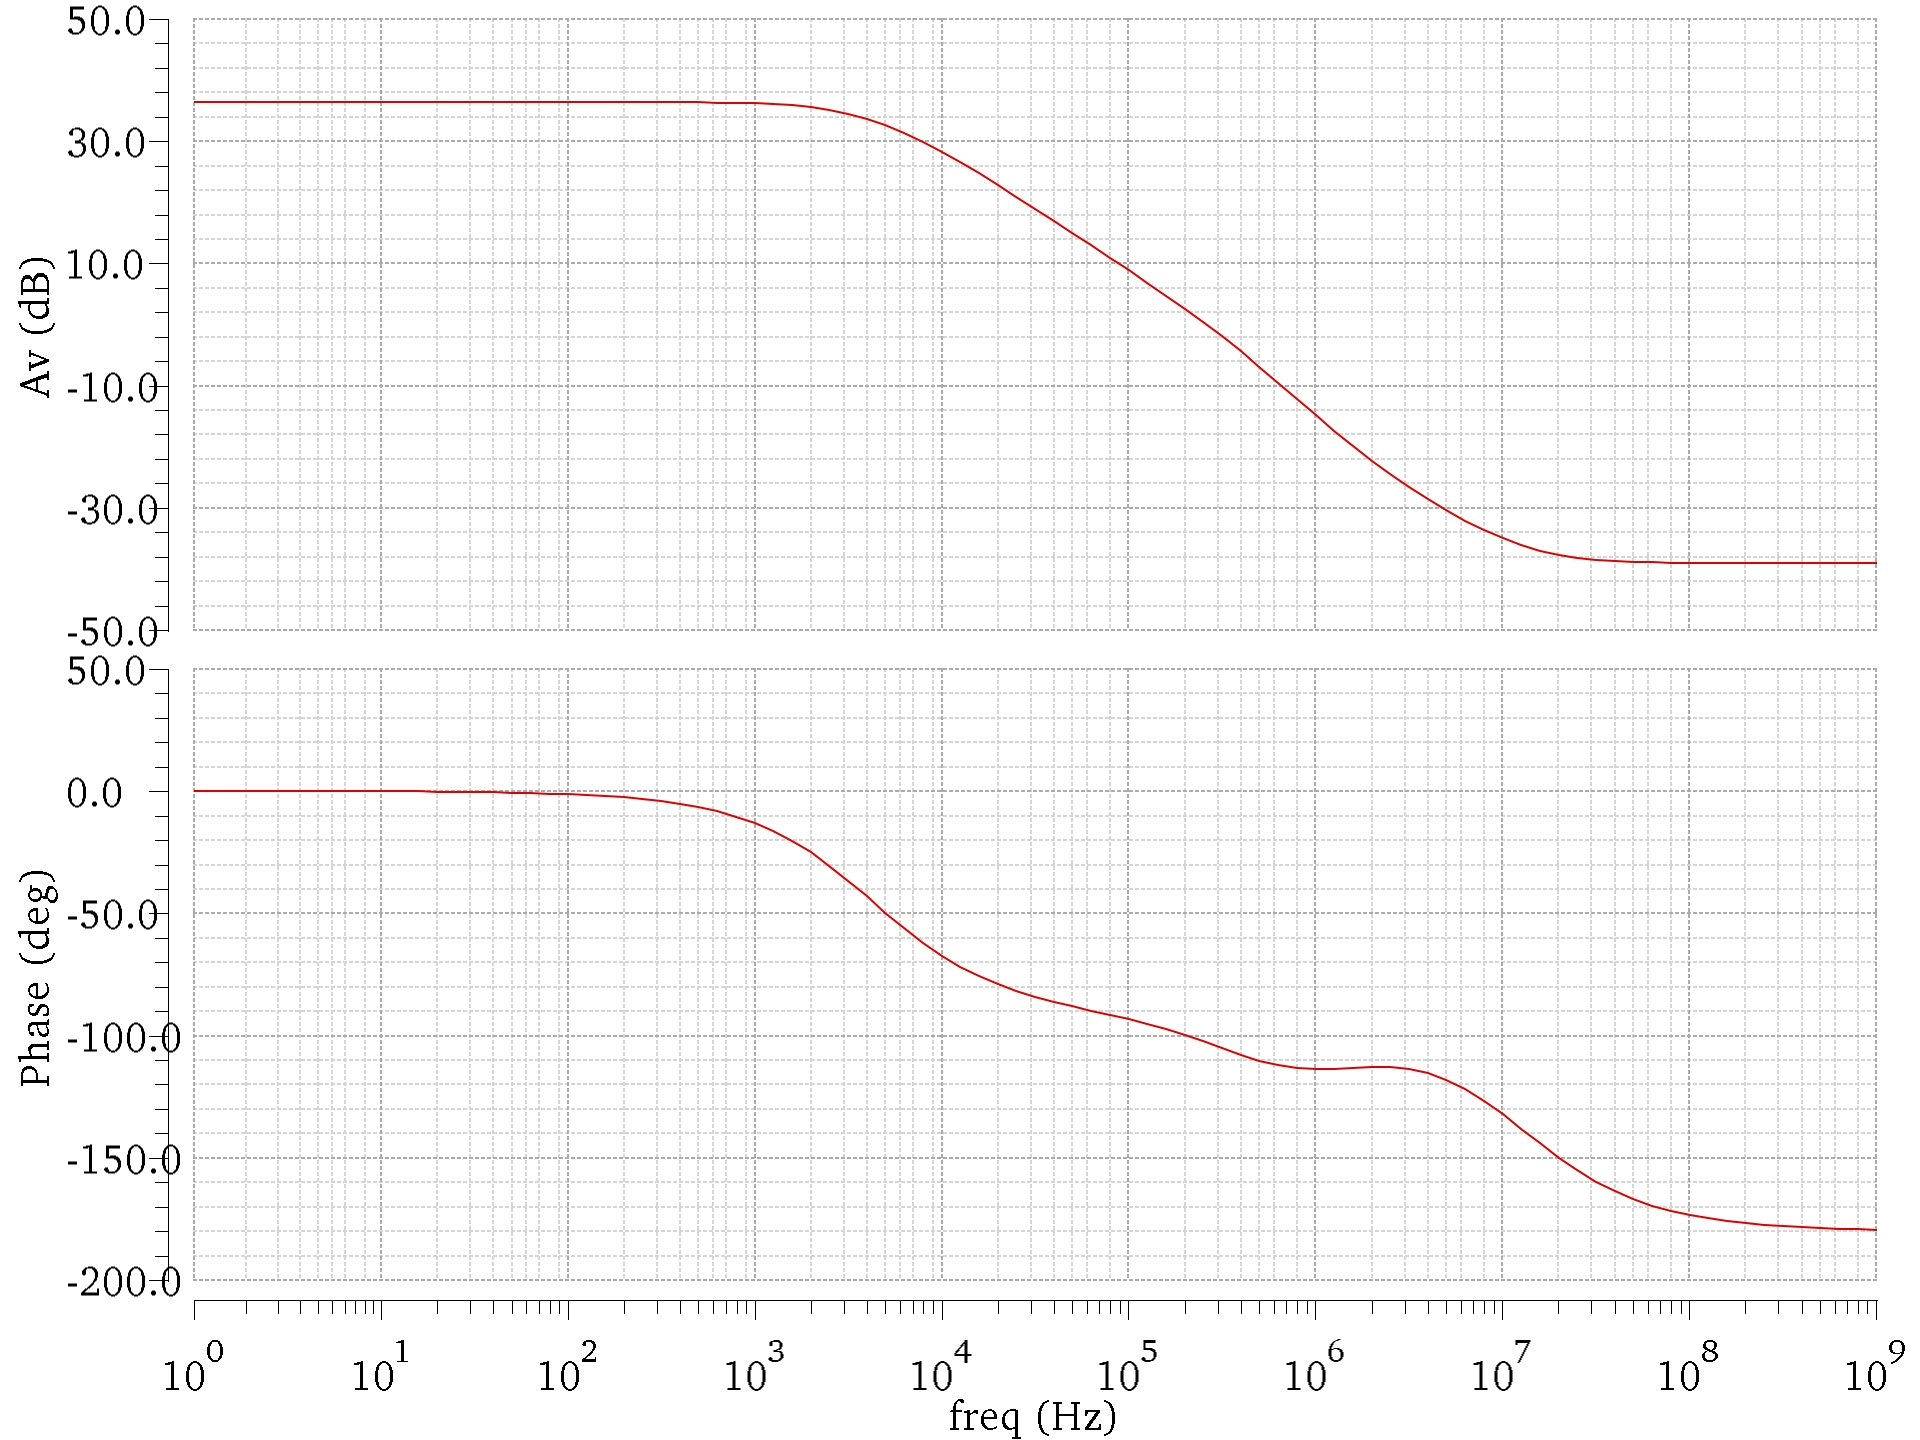
\includegraphics[width=\textwidth]{img/nauta/single/av_ph_0_5V.jpg}
    \caption{Risultati delle simulazioni per il guadagno di tensione ($A_V$) e la fase (Phase) dell'OTA di Nauta a stadio singolo con Valim = 0.5V.}
    \label{fig:results_nauta_single_stage_A_V_phase_0_5V}
\end{figure}
\begin{figure}[H]
    \centering
    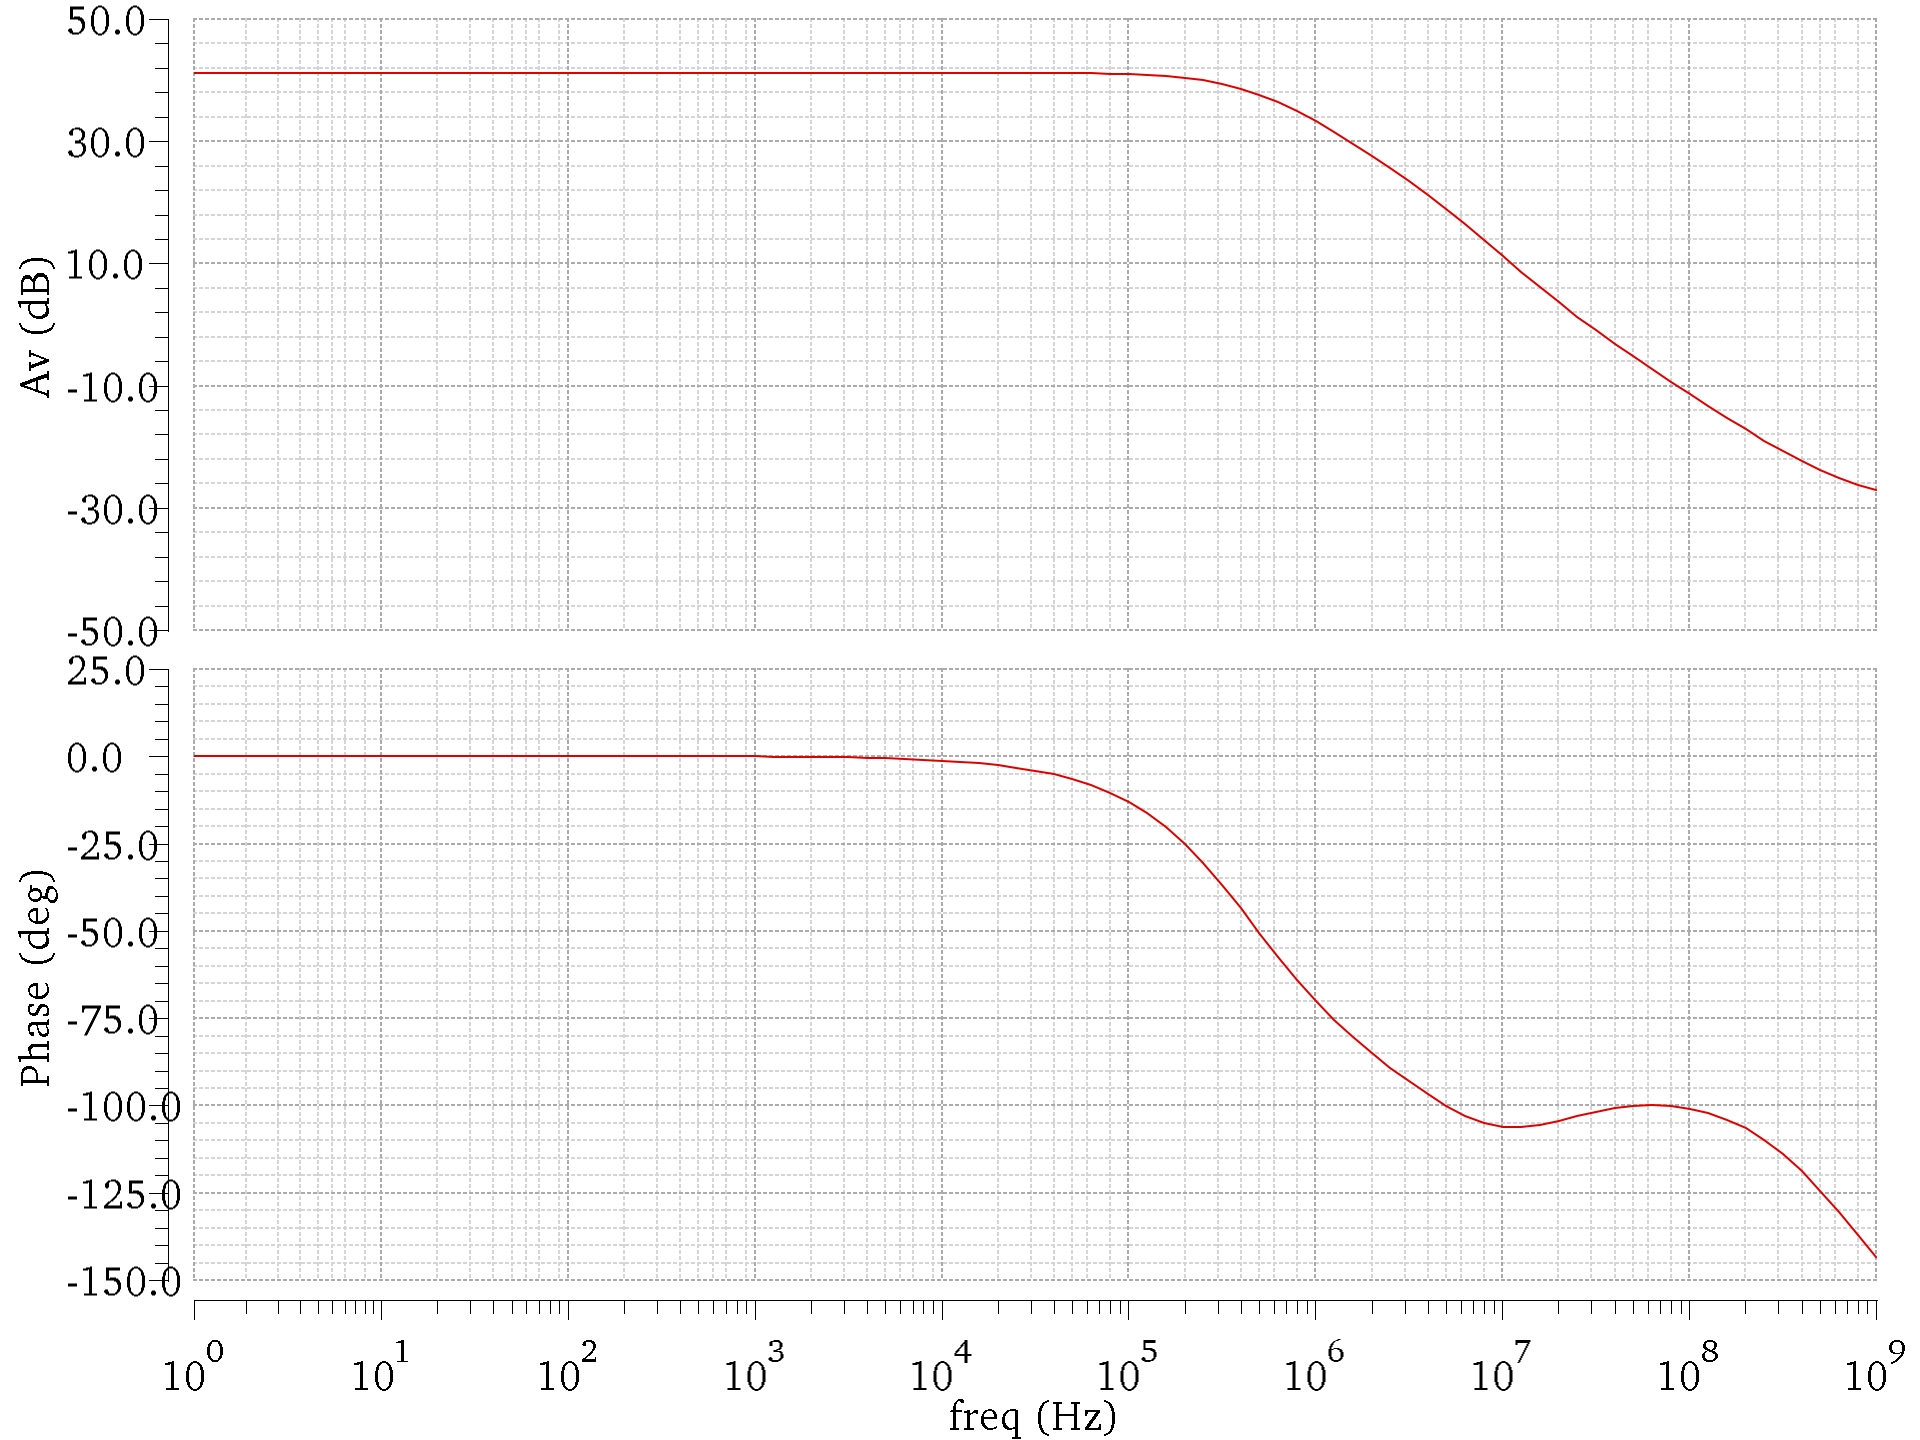
\includegraphics[width=\textwidth]{img/nauta/single/av_ph_1V.jpg}
    \caption{Risultati delle simulazioni per il guadagno di tensione ($A_V$) e la fase (Phase) dell'OTA di Nauta a stadio singolo con Valim = 1V.}
    \label{fig:results_nauta_single_stage_A_V_phase_1V}
\end{figure}
\begin{figure}[H]
    \centering
    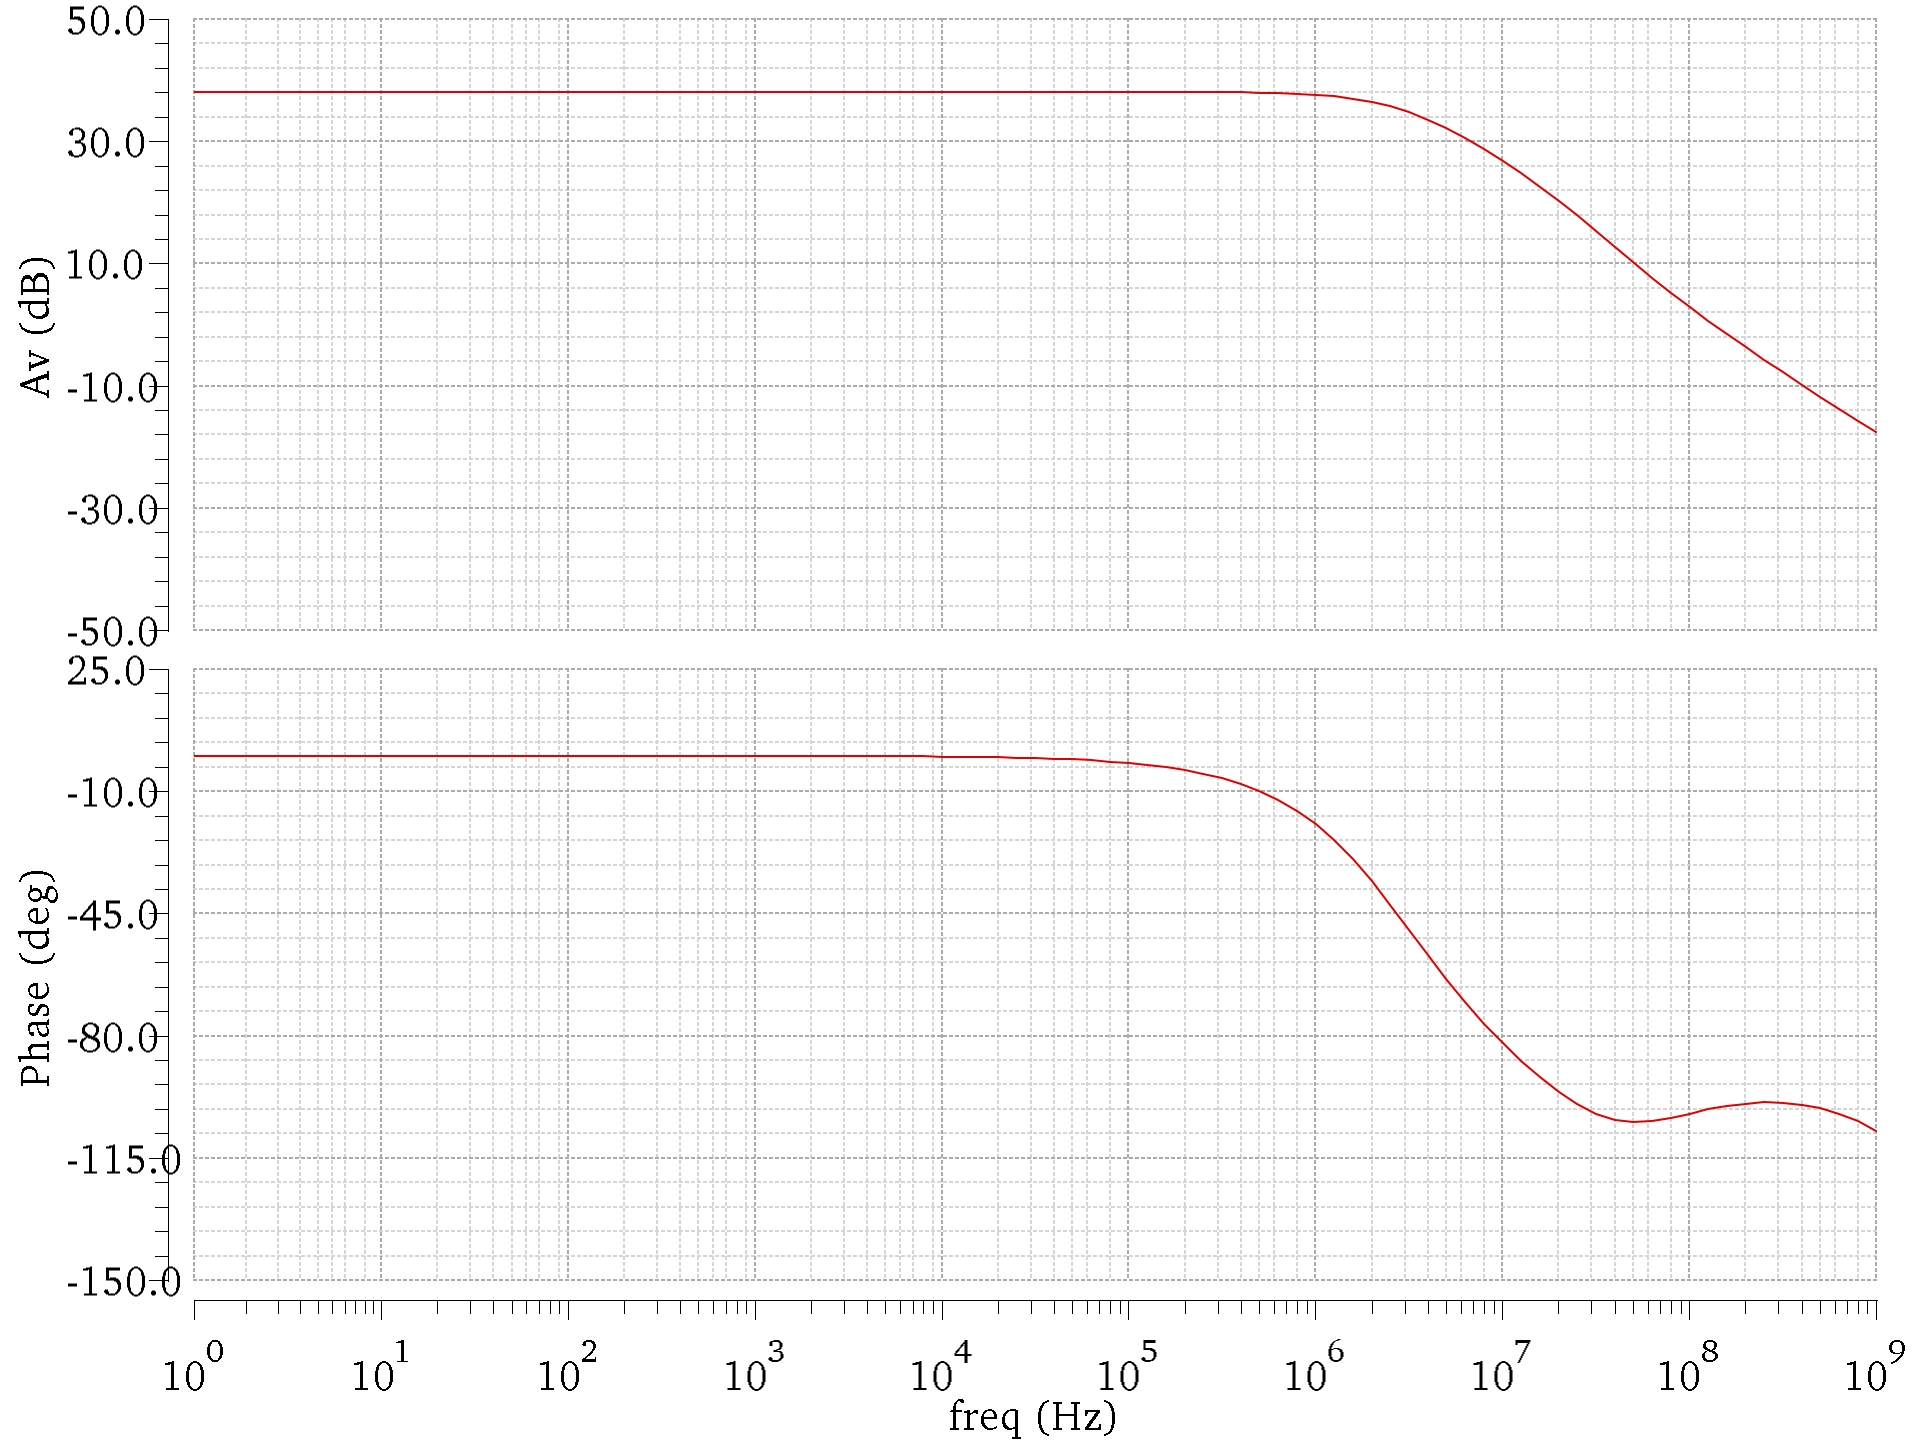
\includegraphics[width=\textwidth]{img/nauta/single/av_ph_1_8V.jpg}
    \caption{Risultati delle simulazioni per il guadagno di tensione ($A_V$) e la fase (Phase) dell'OTA di Nauta a stadio singolo con Valim = 1.8V.}
    \label{fig:results_nauta_single_stage_A_V_phase_1_8V}
\end{figure}


\subsubsection{Phase Margin, Gain Bandwidth Product e Slew Rate}
\label{sec:results_ota_nauta_single_stage_phase_margin_gain_bandwidth_product_slew_rate}

Di seguito vengono riportati i risultati delle simulazioni per il margine di fase (Phase Margin), il prodotto guadagno-banda (Gain Bandwidth Product) e il slew rate (SR). in tabella \ref{tab:results_nauta_single_stage_1pF} sono riportati i risultati per una capacità di carico di 1pF, mentre nella tabella \ref{tab:results_nauta_single_stage_10pF} sono riportati i risultati per una capacità di carico di 10pF.

\begin{table}[H]
    \centering
    \caption{Risultati delle simulazioni per il margine di fase (Phase Margin), il prodotto guadagno-banda (Gain Bandwidth Product) e lo slew rate (SR) dell'OTA di Nauta a stadio singolo con capacità di carico di 1pF.}
    \begin{tabular}{|c|c|c|c|}
        \hline
        \textbf{Valim} & \textbf{Phase Margin} & \textbf{Gain Bandwidth Product} & \textbf{Slew Rate (+/-)} \\ \hline
        0.5V & 71.91° & 352.1 kHz & 3.1/3.1 V/$\mu$s \\ \hline
        1V & 77.63° & 50.36 MHz & 19.2/19.2 V/$\mu$s \\ \hline
        1.8V & 79.16° & 234.8 MHz & 67.4/67.4 V/$\mu$s \\ \hline
    \end{tabular}
    \label{tab:results_nauta_single_stage_1pF}
\end{table}

\begin{table}[H]
    \centering
    \caption{Risultati delle simulazioni per il margine di fase (Phase Margin), il prodotto guadagno-banda (Gain Bandwidth Product) e lo slew rate (SR) dell'OTA di Nauta a stadio singolo con capacità di carico di 10pF.}
    \begin{tabular}{|c|c|c|c|}
        \hline
        \textbf{Valim} & \textbf{Phase Margin} & \textbf{Gain Bandwidth Product} & \textbf{Slew Rate (+/-)} \\ \hline
        0.5V & 50.45° & 35.16 kHz & 0.43/0.43 V/$\mu$s \\ \hline
        1V & 66.07° & 5.01 MHz & 11.2/11.2 V/$\mu$s \\ \hline
        1.8V & 69.98° & 23.38 MHz & 43.8/43.8 V/$\mu$s \\ \hline
    \end{tabular}

    \label{tab:results_nauta_single_stage_10pF}
\end{table}

Come si può notare dall'analisi dei risultati, l'aumento della capacità di carico da 1pF a 10pF produce effetti significativi sulle prestazioni dell'amplificatore:
\begin{itemize}
    \item Il margine di fase diminuisce, riducendosi fino a 50° nel caso peggiore (0.5V);
    \item Il prodotto guadagno-banda si riduce di circa un ordine di grandezza per tutte le tensioni di alimentazione;
    \item Lo slew rate diminuisce per tutte le tensioni di alimentazione.
\end{itemize}
Questo comportamento è perfettamente in linea con la teoria dei circuiti, poiché una maggiore capacità di carico richiede più tempo per essere caricata/scaricata, riducendo così la velocità di risposta complessiva del circuito e alterando la risposta in frequenza.

\subsubsection{Emi rejection}
\label{sec:results_ota_nauta_single_stage_emi_rejection}

Di seguito vengono riportati i risultati delle simulazioni per l'emi rejection dell'OTA di Nauta a stadio singolo. I risultati sono stati ottenuti con una capacità di carico di 1pF.


\begin{figure}[H]
    \centering
    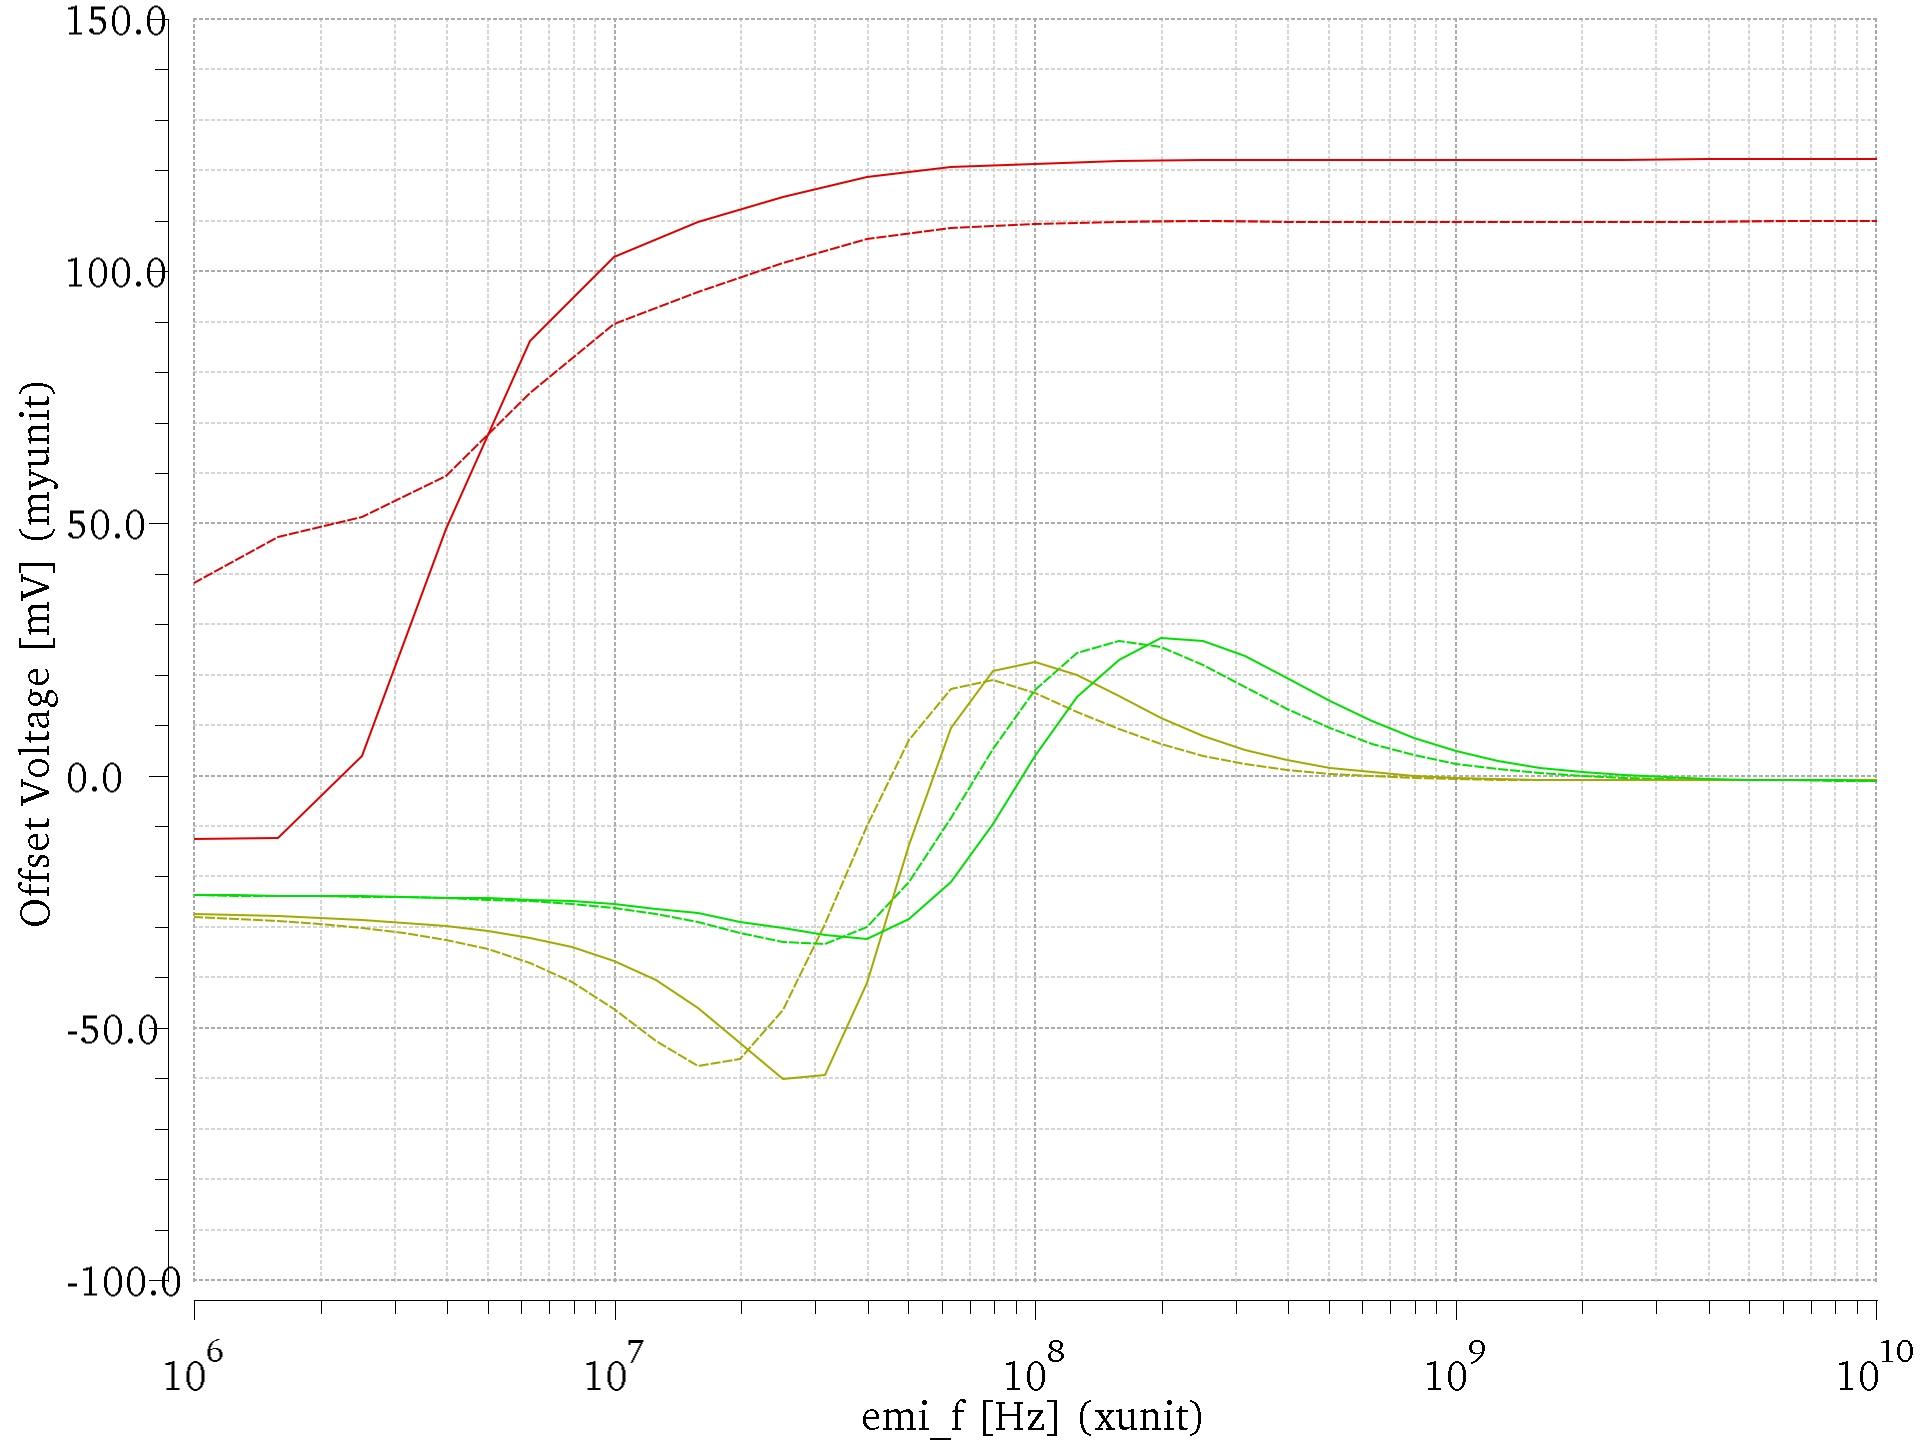
\includegraphics[width=\textwidth]{img/nauta/single/emi_comparison.jpg}
    \vspace{0.2cm}
    \small
    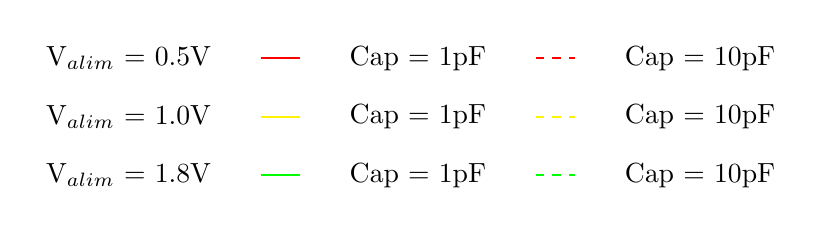
\begin{tikzpicture}
        \matrix[column sep=0.5cm, row sep=0.2cm] {
            \node[right]{V$_{alim}$ = 0.5V}; &
            \draw[red, thick] (0,0) -- (0.5,0); & \node{Cap = 1pF}; &
            \draw[red, thick, dashed] (0,0) -- (0.5,0); & \node{Cap = 10pF}; \\
            \node[right]{V$_{alim}$ = 1.0V}; &
            \draw[yellow, thick] (0,0) -- (0.5,0); & \node{Cap = 1pF}; &
            \draw[yellow, thick, dashed] (0,0) -- (0.5,0); & \node{Cap = 10pF}; \\
            \node[right]{V$_{alim}$ = 1.8V}; &
            \draw[green, thick] (0,0) -- (0.5,0); & \node{Cap = 1pF}; &
            \draw[green, thick, dashed] (0,0) -- (0.5,0); & \node{Cap = 10pF}; \\
        };
    \end{tikzpicture}
    \caption{Risultati delle simulazioni per l'emi rejection dell'OTA di Nauta a stadio singolo}
    \label{fig:results_nauta_single_stage_emi_rejection}
\end{figure}

Si può notare che l'emi rejection dipende fortemente dalla tensione di alimentazione e che tensioni inferiori ad 1V mostrano un comportamento peggiore rispetto a tensioni superiori. Inoltre, si nota che l'emi rejection non è influenzata dalla capacità di carico.

\section{Analisi dei risultati per il Miller OTA a stadio singolo}
\label{sec:results_ota_miller_single_stage}

\subsubsection{Schematico di riferimento per la simulazione}
\label{sec:results_ota_miller_single_stage_reference_schematic}

Lo schematico di riferimento per le simulazioni perl'OTA di Miller a stadio singolo utilizzato è mostrato nella figura \ref{fig:schematic_miller_single_stage}. Anche in questo caso, la capacità di carico è di 1pF.
\begin{figure}[H]
    \centering
    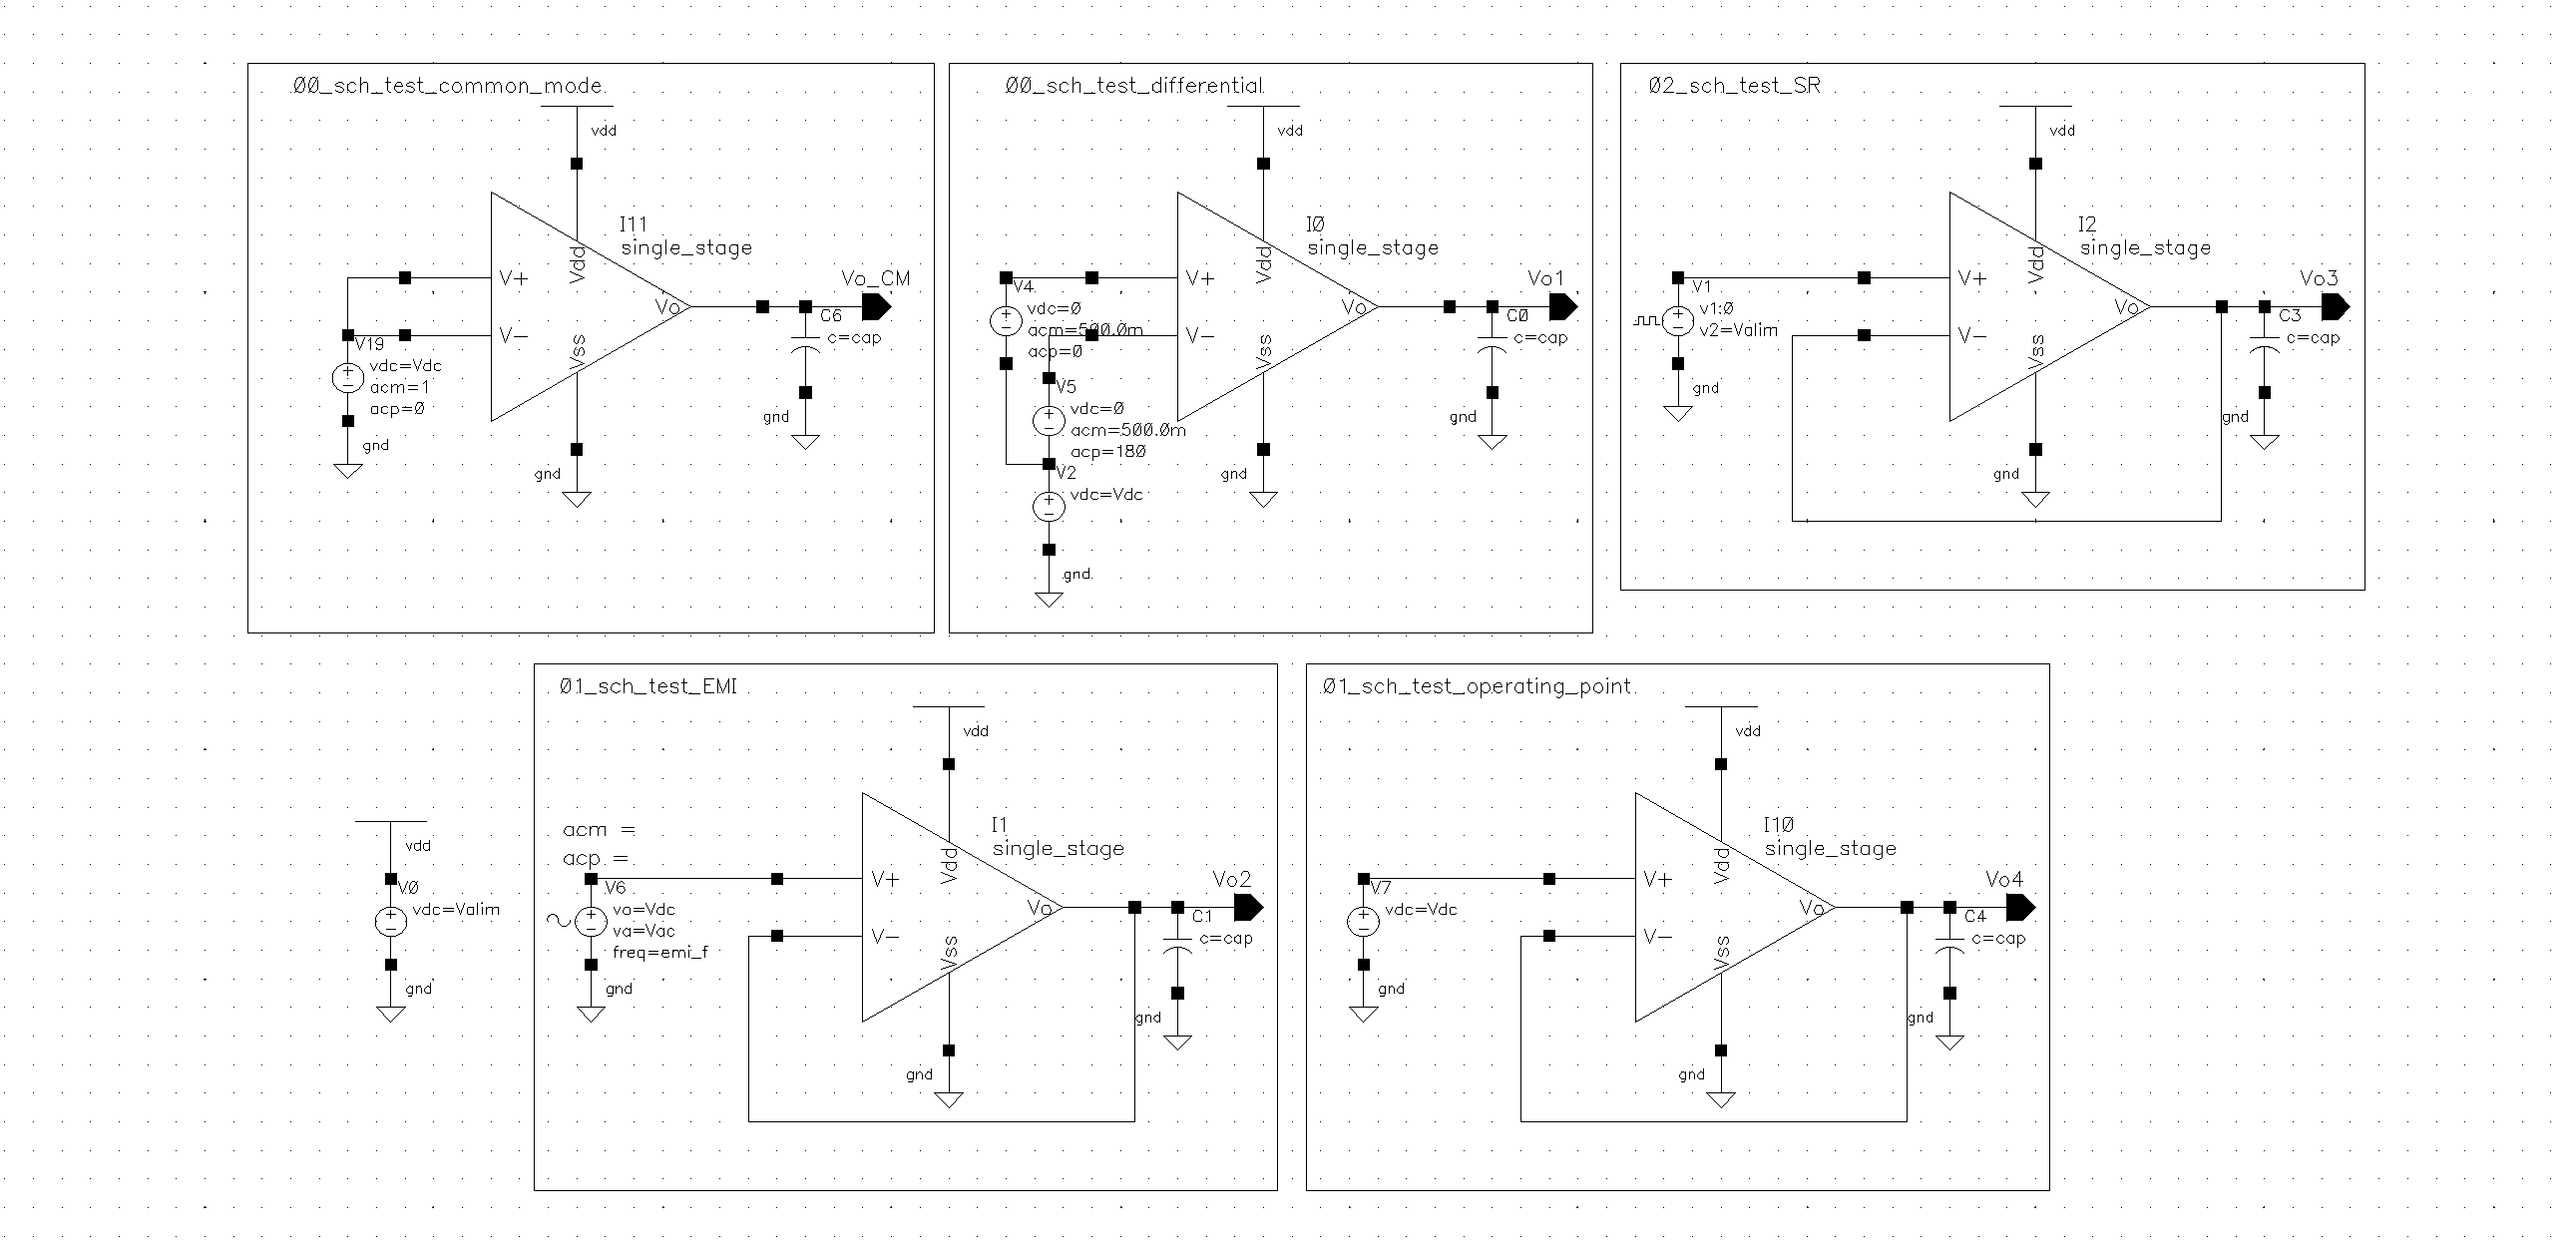
\includegraphics[width=\textwidth]{img/miller/single/sim_miller_single.png}
    \caption{Schematico di riferimento per l'OTA di Miller a stadio singolo.}
    \label{fig:schematic_miller_single_stage}
\end{figure}

In figura \ref{fig:schematic_miller_single_stage_inverter} è mostrato lo schematico di riferimento per la cella \textit{single\_stage} dell'OTA di Miller a stadio singolo. Tutti i parametri indicati sono riportati nella Tabella \ref{tab:component_sizing_miller_single_stage}. 

\begin{figure}[H]
    \centering
    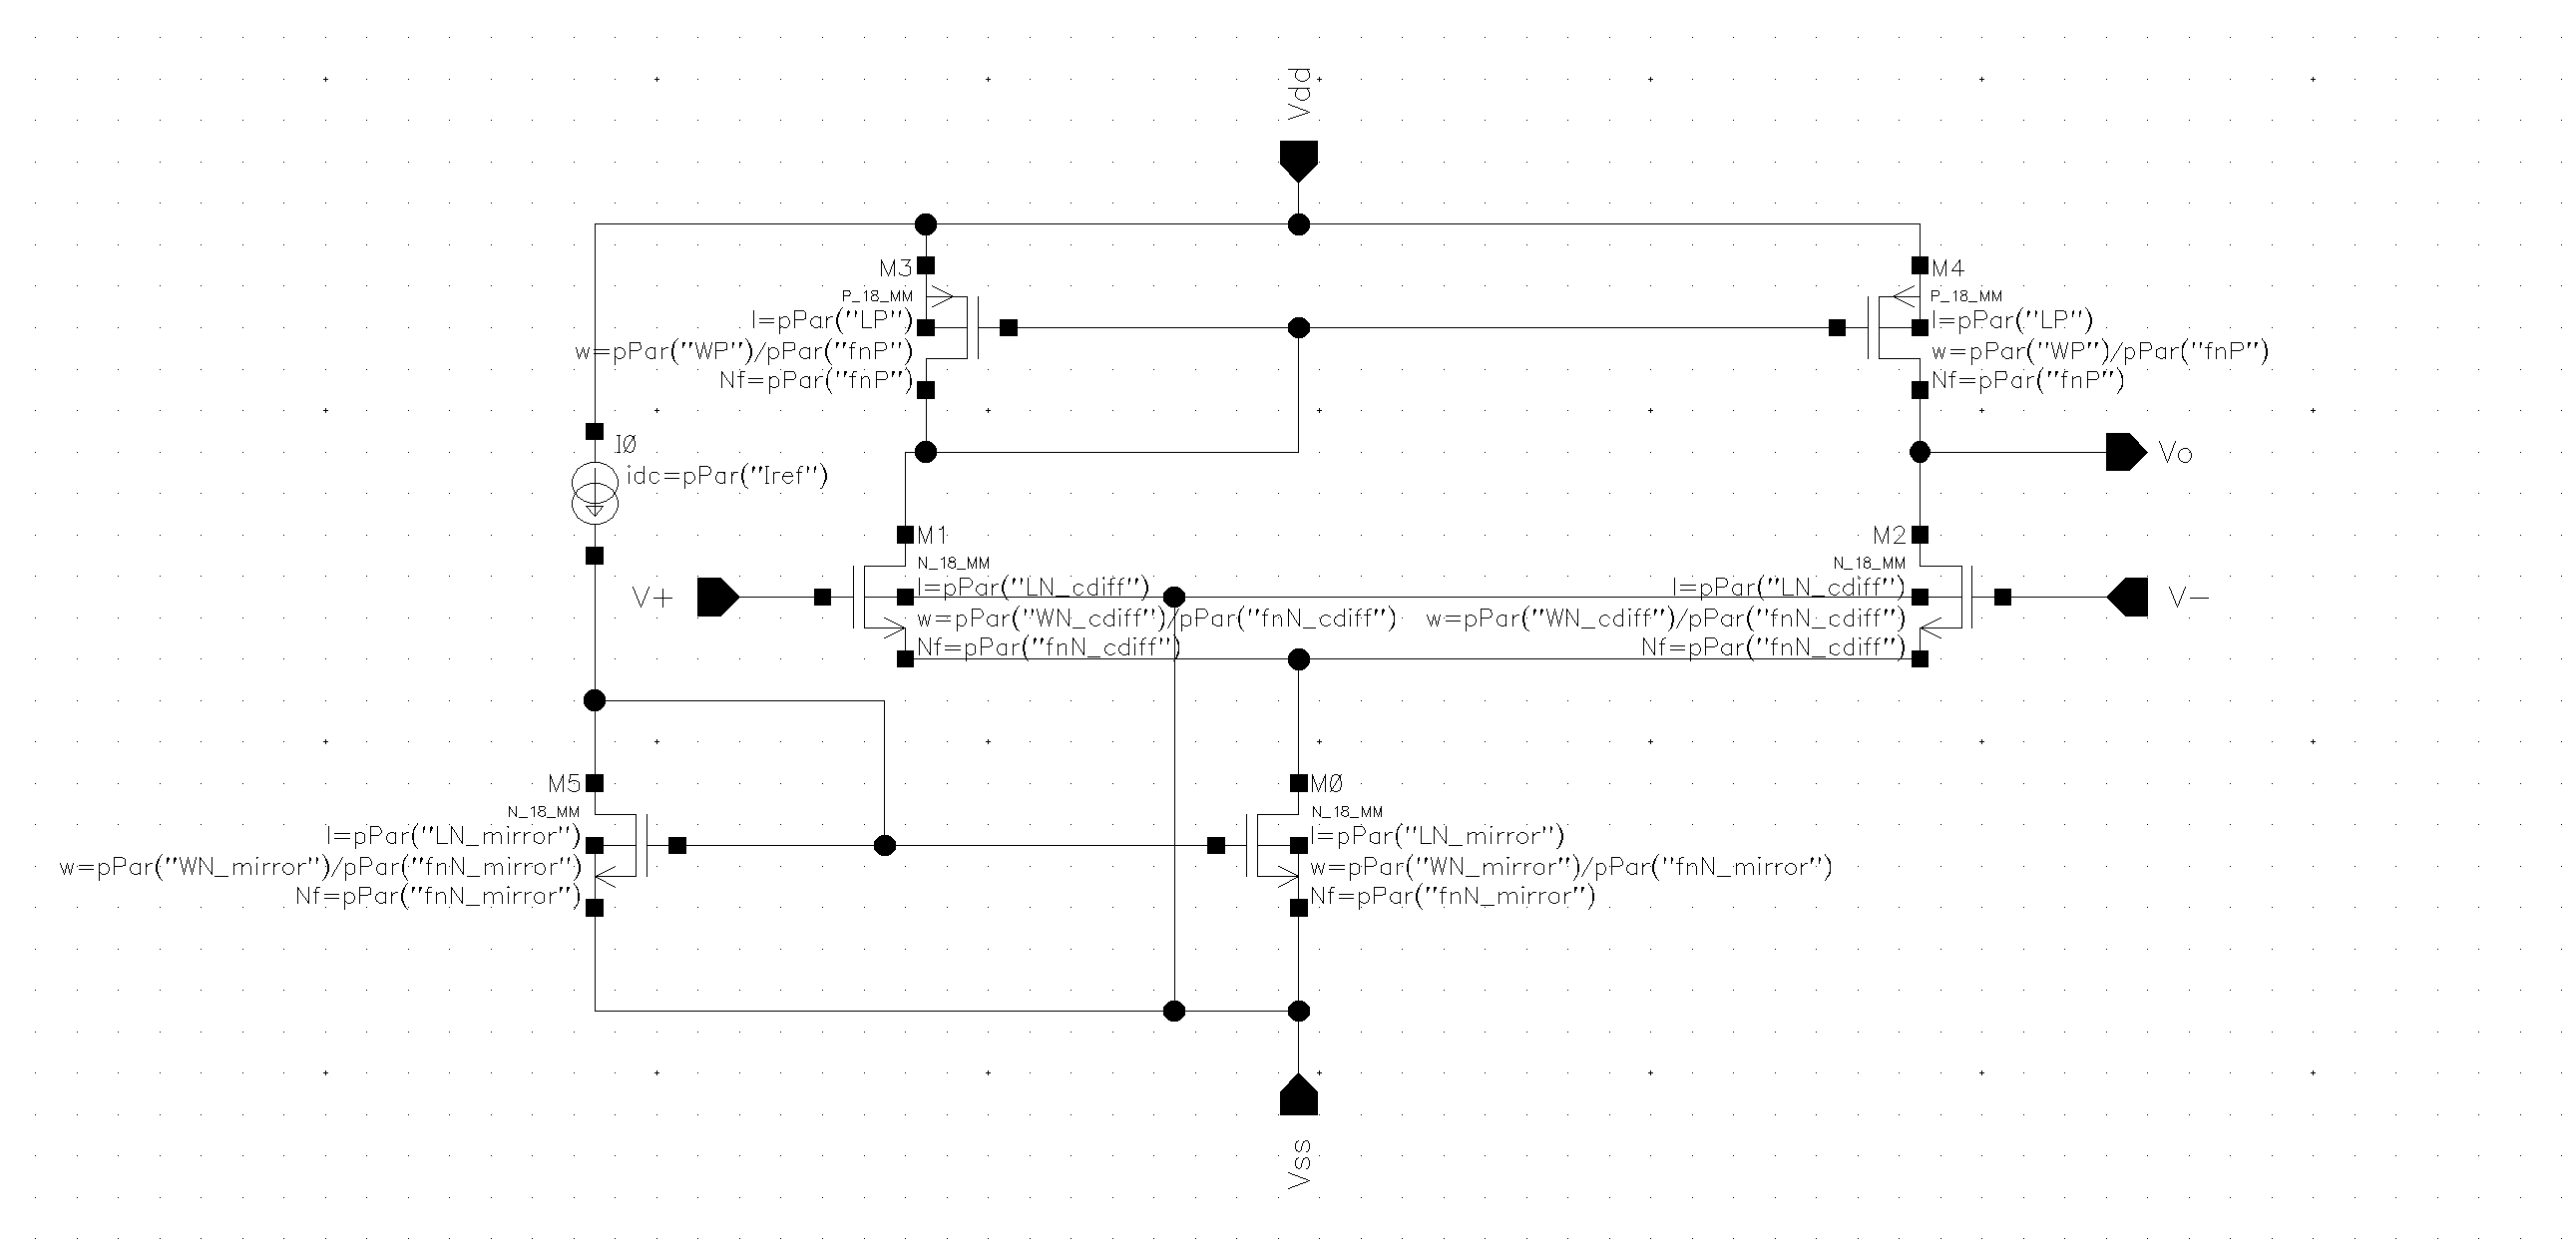
\includegraphics[width=\textwidth]{img/miller/single/sch_miller_single.png}
    \caption{Schematico del blocco \textit{single\_stage} per l'OTA di Miller a stadio singolo.}
    \label{fig:schematic_miller_single_stage_inverter}
\end{figure}

\subsubsection{Dimensionamento dei componenti}
\label{sec:results_ota_miller_single_stage_component_sizing}

\begin{table}[H]
    \centering
    \begin{tabular}{c|c|c|}
        \cline{2-3}
        & \textbf{Valim = 1V} & \textbf{Valim = 1.8V} \\ \hline
        \multicolumn{3}{|c|}{\textbf{Parametri di simulazione}} \\ \hline
        \multicolumn{1}{|c|}{$L_{N\_cdiff}$} & 1$\mu$m & 1$\mu$m \\ \hline
        \multicolumn{1}{|c|}{$W_{N\_cdiff}$} & 24$\mu$m & 24$\mu$m \\ \hline
        \multicolumn{1}{|c|}{$\#finger_{N\_cdiff}$} & 8 & 8 \\ \hline
        \multicolumn{1}{|c|}{$L_{N\_mirror}$} & 1$\mu$m & 1$\mu$m \\ \hline
        \multicolumn{1}{|c|}{$W_{N\_mirror}$} & 24$\mu$m & 24$\mu$m \\ \hline
        \multicolumn{1}{|c|}{$\#finger_{N\_mirror}$} & 8 & 8 \\ \hline
        \multicolumn{1}{|c|}{fnP} & 8 & 8 \\ \hline
        \multicolumn{1}{|c|}{LP} & 1$\mu$m & 1$\mu$m \\ \hline
        \multicolumn{1}{|c|}{WP} & 32$\mu$m & 32$\mu$m \\ \hline
        \multicolumn{1}{|c|}{Iref} & 20$\mu$A & 20$\mu$A \\ \hline
        \multicolumn{3}{|c|}{\textbf{Risultati simulazione}}  \\ \hline
        \multicolumn{1}{|c|}{Ipol} & 17.02$\mu$A & 13.95$\mu$A \\ \hline
        \multicolumn{1}{|c|}{I0/M0 region} & 2 & 2 \\ \hline
        \multicolumn{1}{|c|}{I0/M1 region} & 2 & 2 \\ \hline
        \multicolumn{1}{|c|}{I0/M2 region} & 2 & 2 \\ \hline
        \multicolumn{1}{|c|}{I0/M3 region} & 2 & 2 \\ \hline
        \multicolumn{1}{|c|}{I0/M4 region} & 2 & 2 \\ \hline
        \multicolumn{1}{|c|}{I0/M5 region} & 2 & 2 \\ \hline
        \multicolumn{1}{|c|}{AV(0)} & 36.56dB & 36.47dB \\ \hline
        \multicolumn{1}{|c|}{f$_c$} & 389.3kHz & 457.1kHz \\ \hline
        \multicolumn{1}{|c|}{f$_o$} & 24.28MHz & 28.11MHz \\ \hline
    \end{tabular}
    \caption{Dimensionamento dei componenti dell'OTA di Miller a stadio singolo. Tutti i risultati sono stati ottenuti con una capacità di carico di 1pF.}
    \label{tab:component_sizing_miller_single_stage}
\end{table}

\subsubsection{Av, Phase, CMRR e CMR}
\label{sec:results_ota_miller_single_stage_A_V_phase_CMRR_CMR}

Di seguito vengono riportati i risultati delle simulazioni per il guadagno di tensione ($A_V$), la fase (Phase).

\begin{figure}[H]
    \centering
    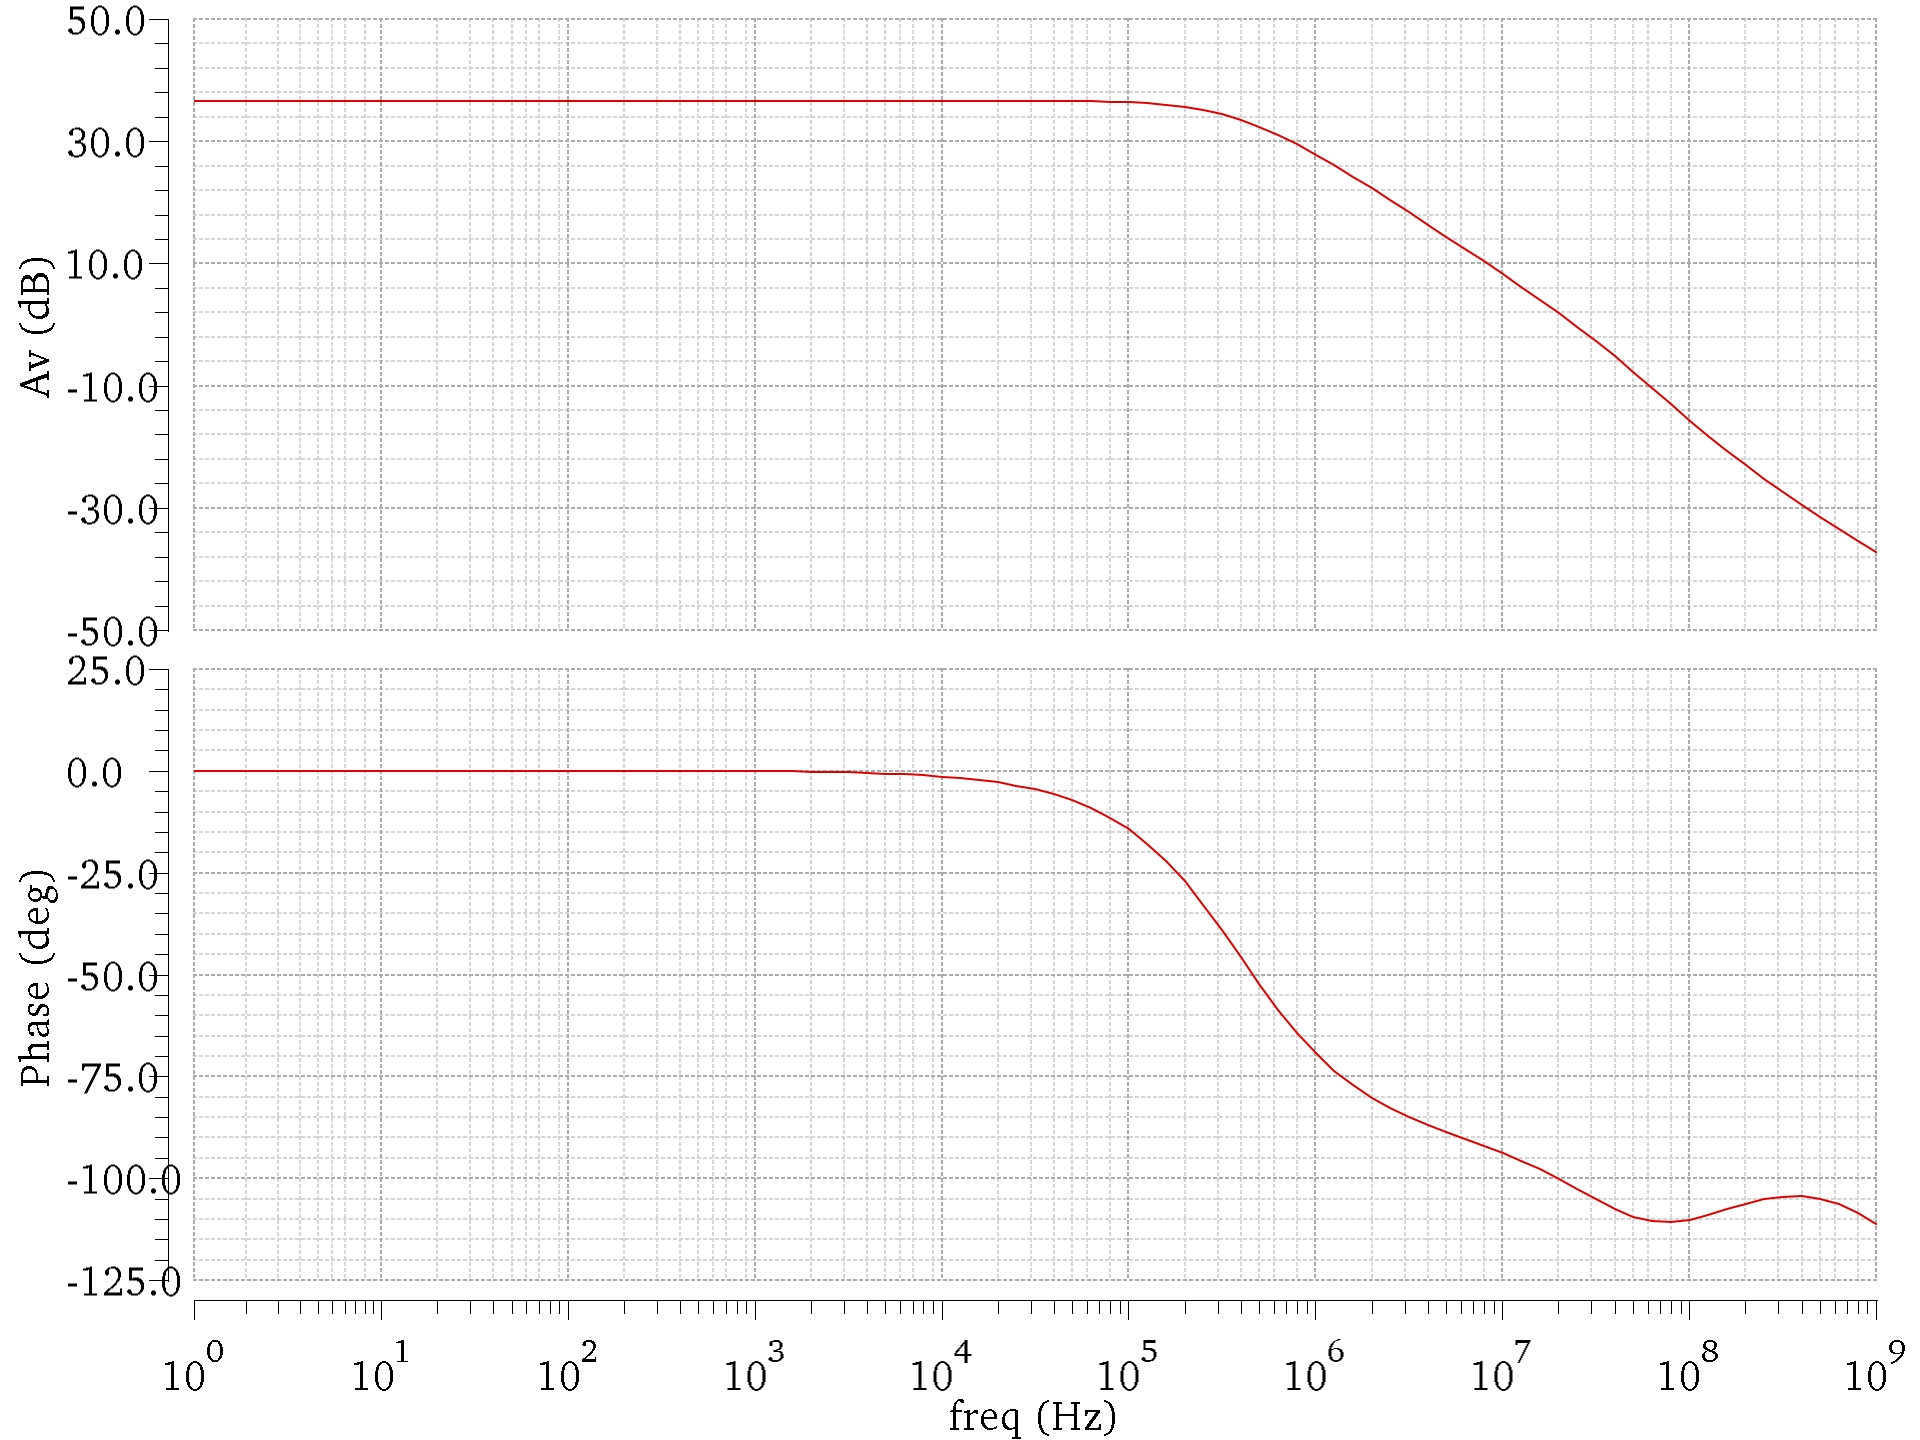
\includegraphics[width=\textwidth]{img/miller/single/av_phase_1V.jpg}
    \caption{Risultati delle simulazioni per il guadagno di tensione ($A_V$) e la fase (Phase) dell'OTA di Miller a stadio singolo con Valim = 1V.}
    \label{fig:results_miller_single_stage_A_V_phase_1V}
\end{figure}

\begin{figure}[H]
    \centering
    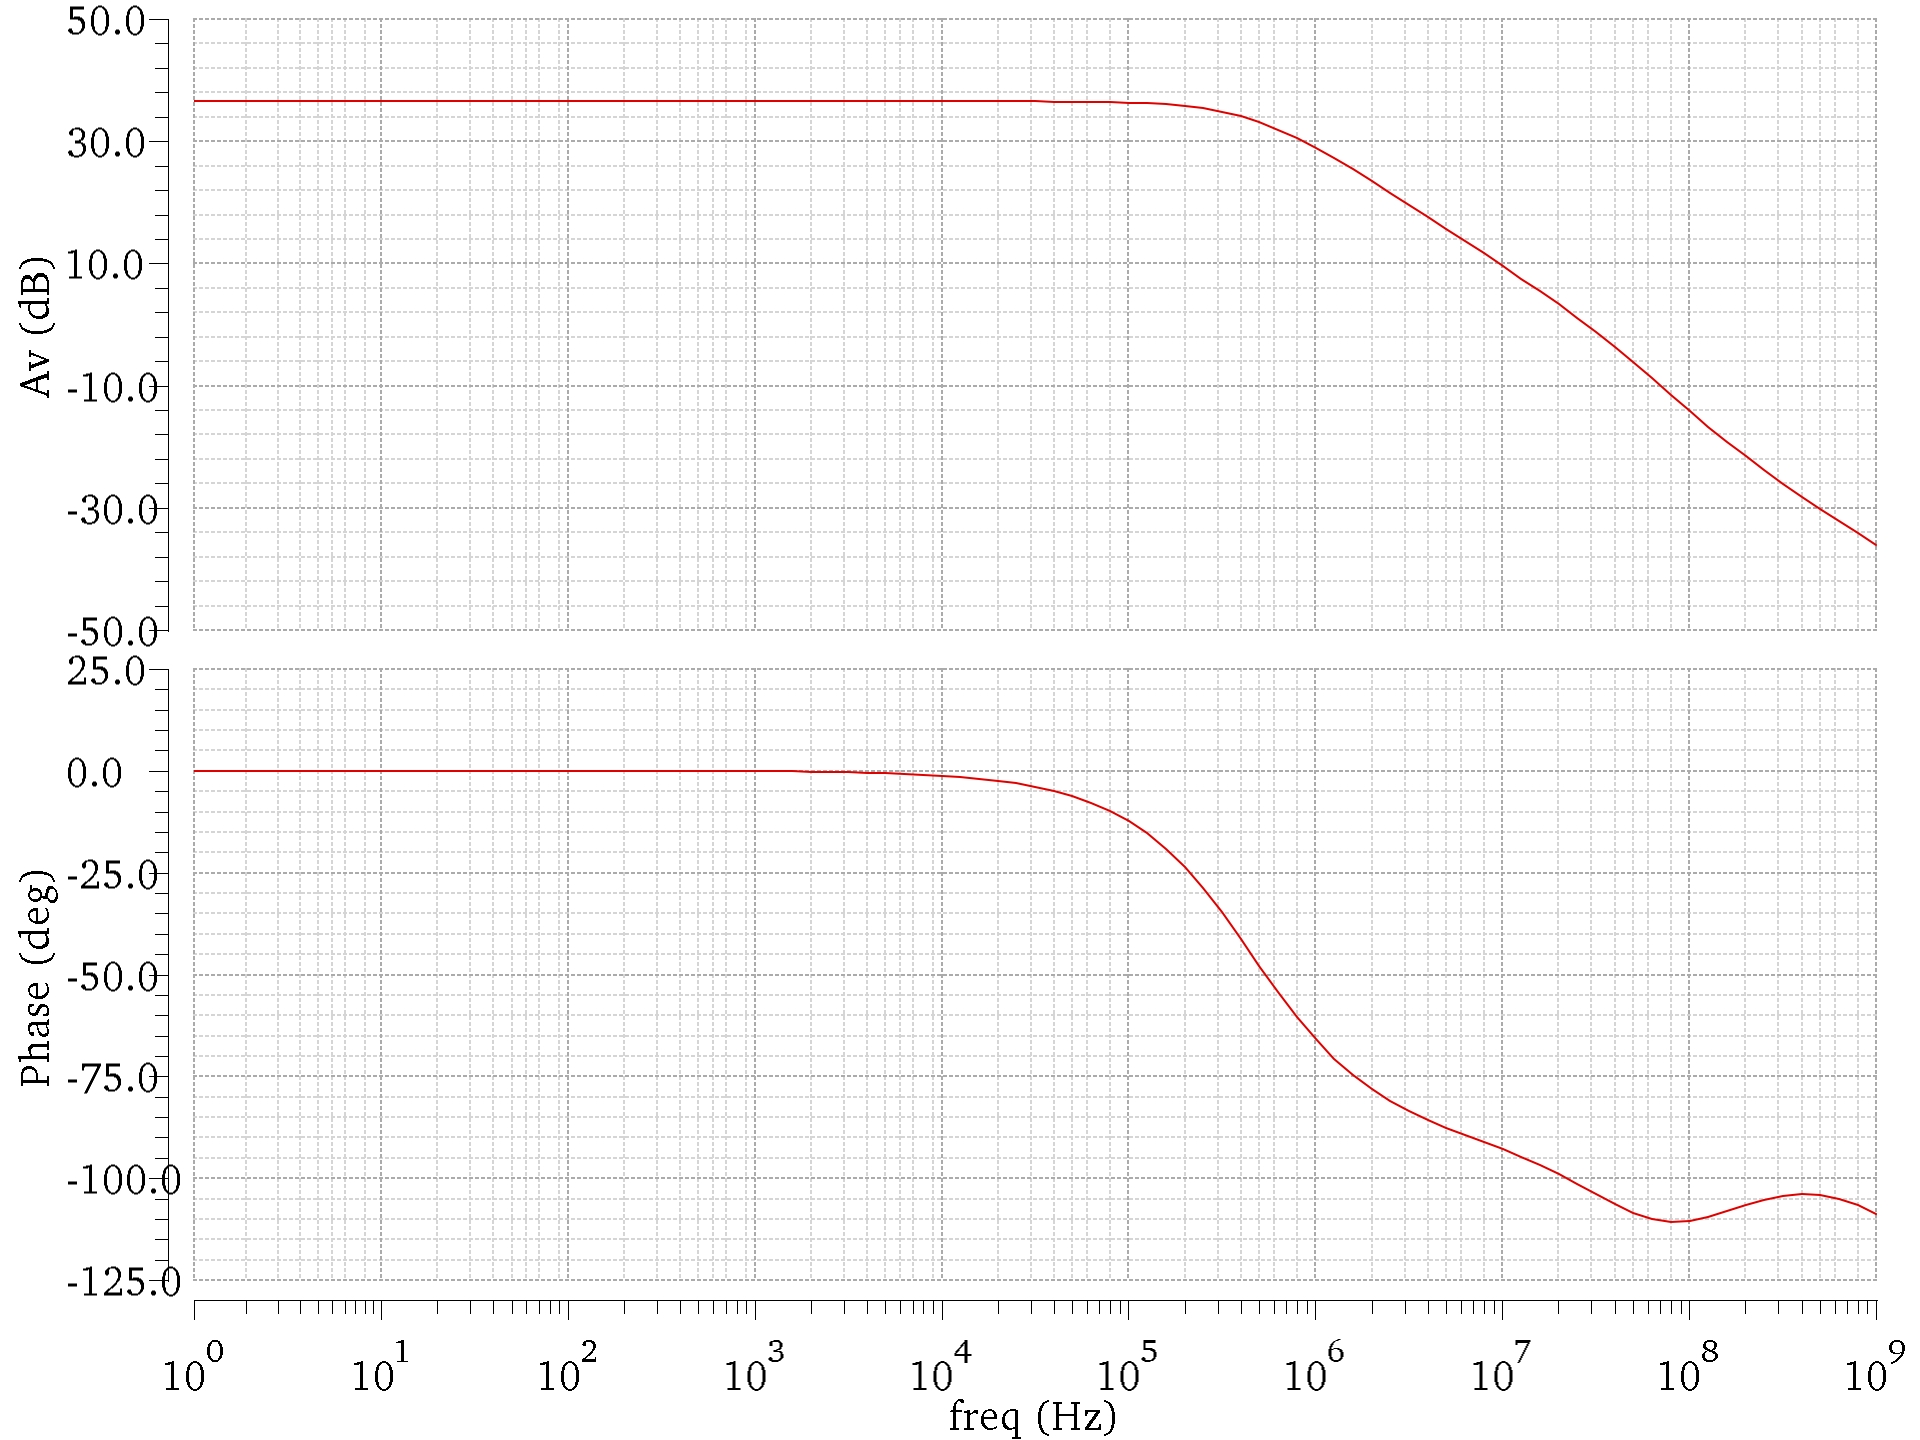
\includegraphics[width=\textwidth]{img/miller/single/av_phase_1_8V.jpg}
    \caption{Risultati delle simulazioni per il guadagno di tensione ($A_V$) e la fase (Phase) dell'OTA di Miller a stadio singolo con Valim = 1.8V.}
    \label{fig:results_miller_single_stage_A_V_phase_1_8V}
\end{figure}

Dalle figure \ref{fig:results_miller_single_stage_A_V_phase_1V} e \ref{fig:results_miller_single_stage_A_V_phase_1_8V} si può notare che il guadagno di tensione ($A_V$) è relativamente costante per frequenze inferiori a 1MHz, mentre la fase (Phase) mostra un comportamento più complesso. In particolare, si osserva una diminuzione della fase a frequenze superiori a 1MHz, con un margine di fase (Phase Margin) di circa 77° per Valim = 1V e 79° per Valim = 1.8V.
Inoltre, si nota che il guadagno di tensione ($A_V$) è leggermente più elevato per Valim = 1.8V rispetto a Valim = 1V, il che è in linea con le aspettative, poiché un'alimentazione più alta consente una maggiore escursione di tensione per l'amplificatore.

Di seguito vengono riportati i risultati delle simulazioni per il rapporto di reiezione al modo comume (CMRR) e il range di modo comune (CMR).

\begin{figure}[H]
    \centering
    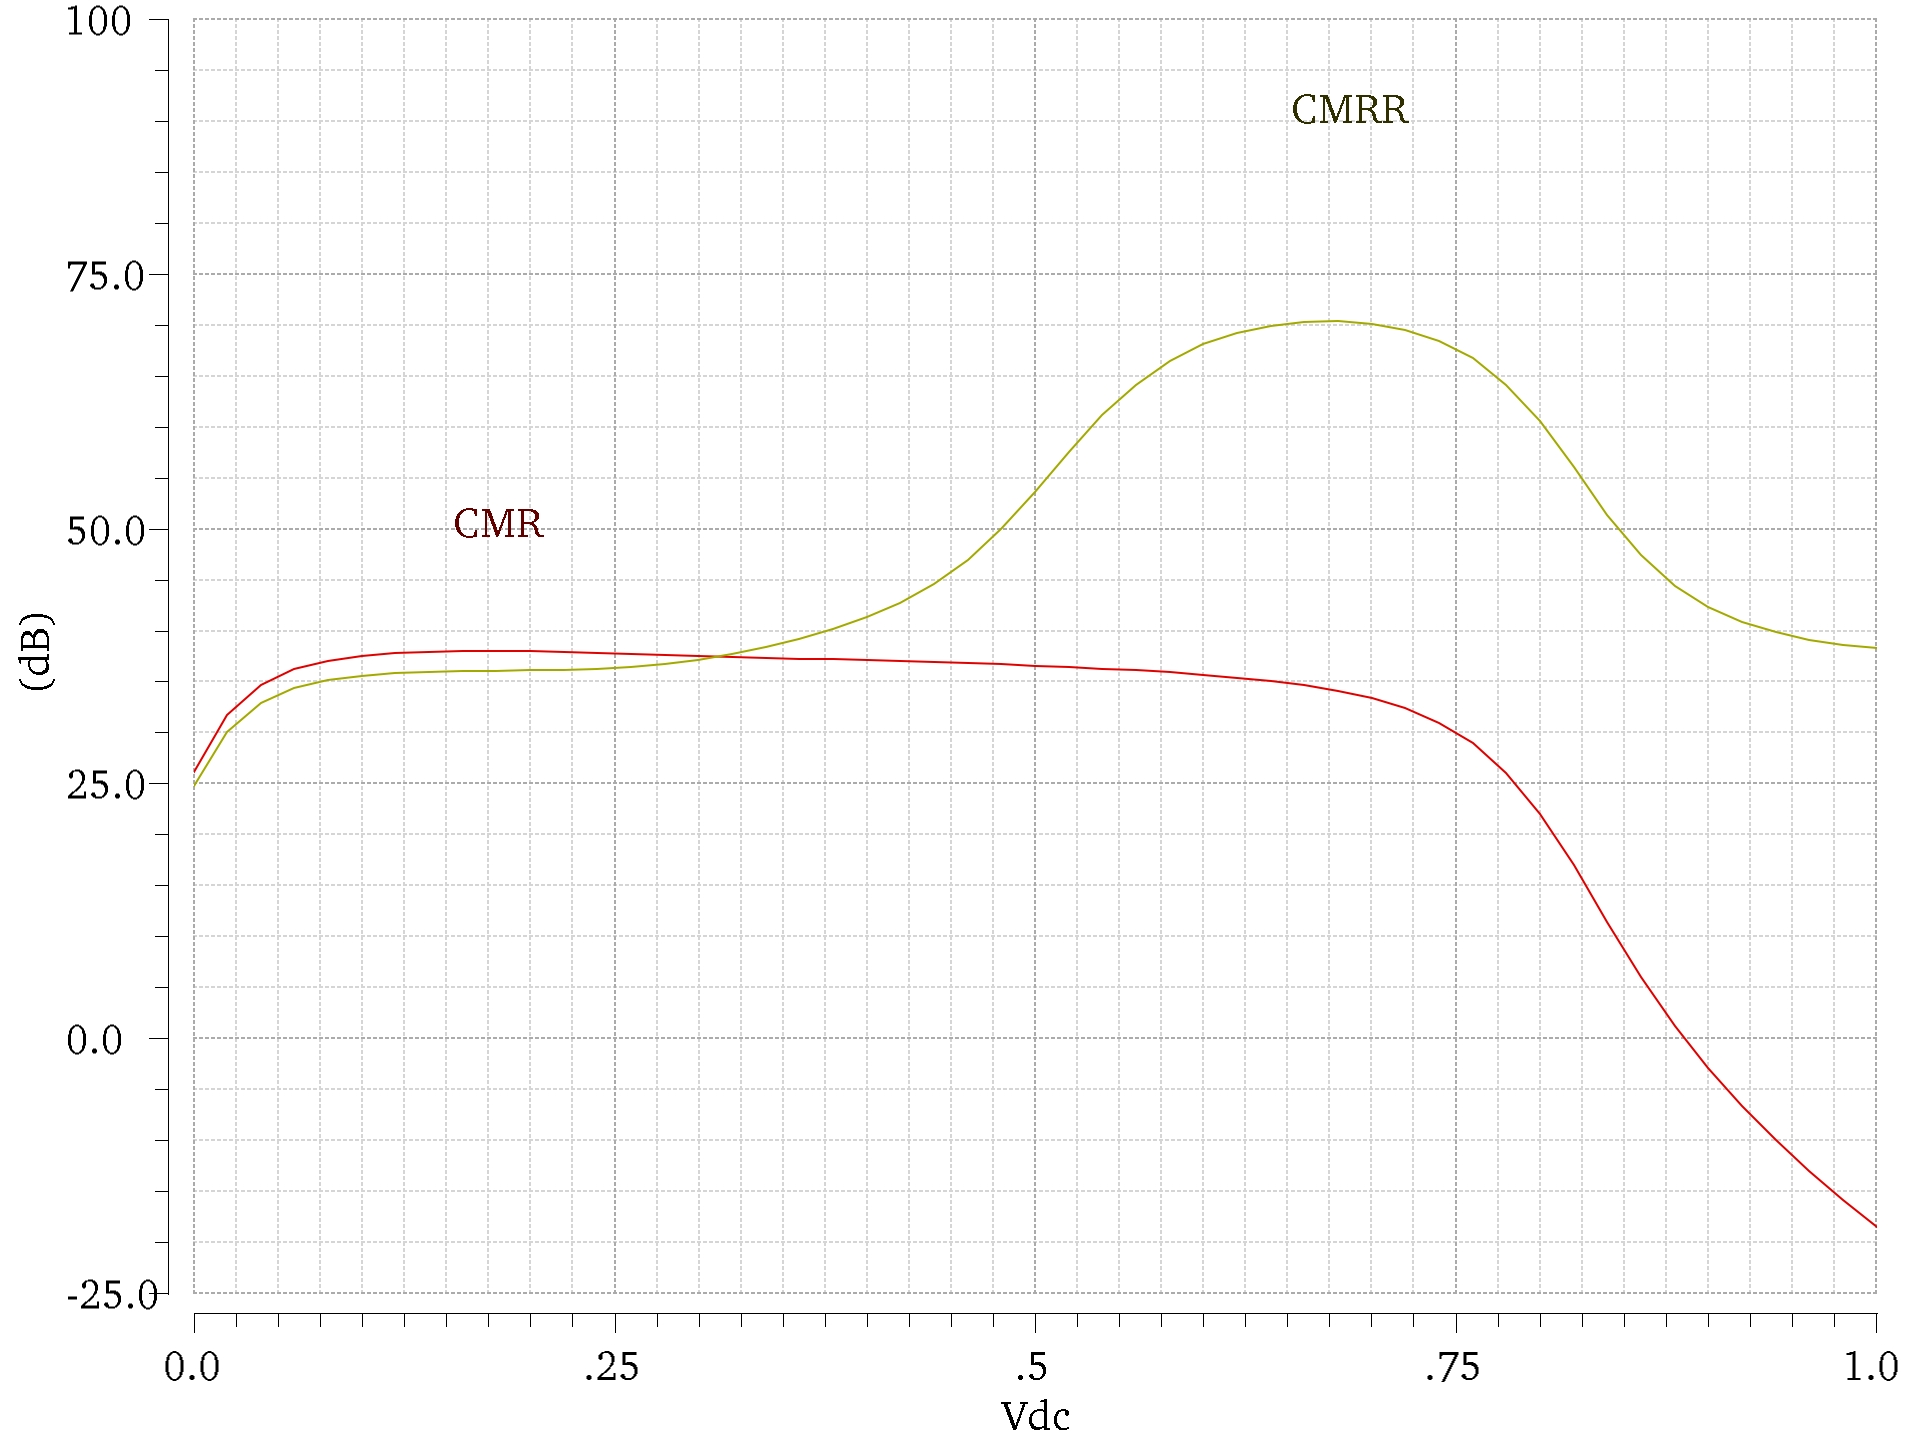
\includegraphics[width=\textwidth]{img/miller/single/cmr_cmrr_1V.jpg}
    \caption{Risultati delle simulazioni per il rapporto di reiezione al modo comume (CMRR) e il range di modo comune (CMR) dell'OTA di Miller a stadio singolo con Valim = 1V.}
    \label{fig:results_miller_single_stage_CMRR_CMR_1V}
\end{figure}

\begin{figure}[H]
    \centering
    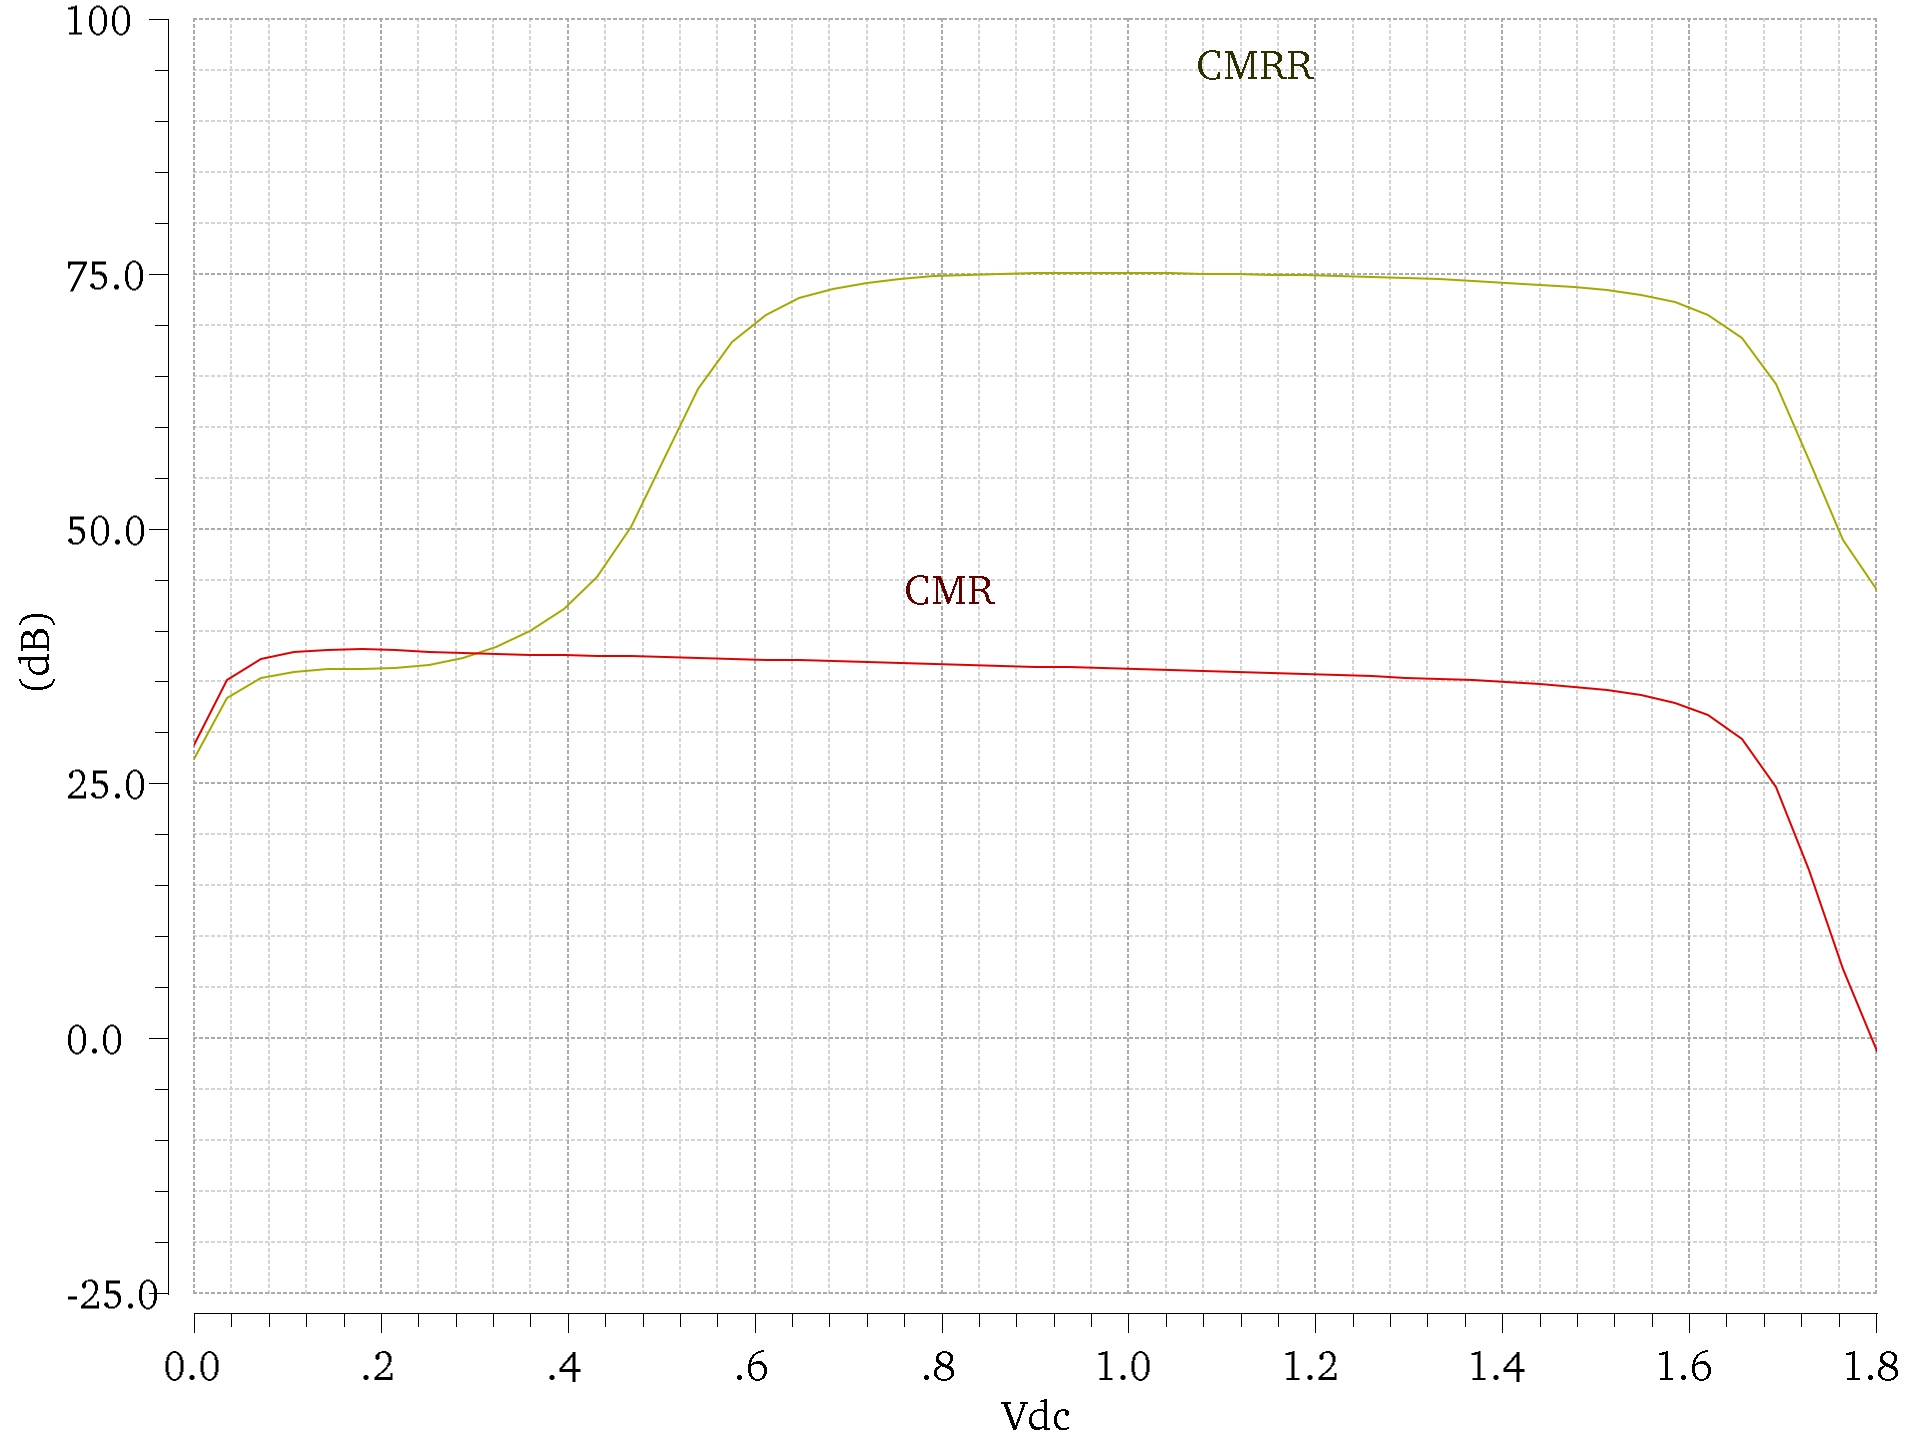
\includegraphics[width=\textwidth]{img/miller/single/cmr_cmrr_1_8V.jpg}
    \caption{Risultati delle simulazioni per il rapporto di reiezione al modo comume (CMRR) e il range di modo comune (CMR) dell'OTA di Miller a stadio singolo con Valim = 1.8V.}
    \label{fig:results_miller_single_stage_CMRR_CMR_1_8V}
\end{figure}

Dalle figure \ref{fig:results_miller_single_stage_CMRR_CMR_1V} e \ref{fig:results_miller_single_stage_CMRR_CMR_1_8V} si può notare che il CMR è relativamente costante per quasi tutto il range di tensioni di modo comune, mentre il CMRR mostra un comportamento più complesso seppur mantenendo un buon valore per le tensioni di modo comune intorno alla metà della dinamica.

\subsubsection{Phase Margin, Gain Bandwidth Product e Slew Rate}
\label{sec:results_ota_miller_single_stage_phase_margin_gain_bandwidth_product_slew_rate}

Di seguito vengono riportati i risultati delle simulazioni per il margine di fase (Phase Margin), il prodotto guadagno-banda (Gain Bandwidth Product) e lo slew rate (SR).

\begin{table}[H]
    \centering
    \begin{tabular}{|c|c|c|c|}
        \hline
        \textbf{Valim} & \textbf{Phase Margin} & \textbf{Gain Bandwidth Product} & \textbf{Slew Rate (+/-)} \\ \hline
        1V & 77.88° & 26.3 MHz & 16.7/16.7 V/$\mu$s \\ \hline
        1.8V & 77.58° & 30.61 MHz & 20.8/20.8 V/$\mu$s \\ \hline
    \end{tabular}
    \caption{Risultati delle simulazioni per il margine di fase (Phase Margin), il prodotto guadagno-banda (Gain Bandwidth Product) e lo slew rate (SR) dell'OTA di Miller a stadio singolo con capacità di carico di 1pF.}
    \label{tab:results_miller_single_stage_1pF}
\end{table}

\begin{table}[H]
    \centering
    \begin{tabular}{|c|c|c|c|}
        \hline
        \textbf{Valim} & \textbf{Phase Margin} & \textbf{Gain Bandwidth Product} & \textbf{Slew Rate (+/-)} \\ \hline
        1V & 89.11° & 2.83 MHz & 1.9/1.9 V/$\mu$s \\ \hline
        1.8V & 89.04° & 3.28 MHz & 2.2/2.2 V/$\mu$s \\ \hline
    \end{tabular}
    \caption{Risultati delle simulazioni per il margine di fase (Phase Margin), il prodotto guadagno-banda (Gain Bandwidth Product) e lo slew rate (SR) dell'OTA di Miller a stadio singolo con capacità di carico di 10pF.}
    \label{tab:results_miller_single_stage_10pF}
\end{table}

L'analisi dei risultati ottenuti per l'amplificatore Miller a singolo stadio evidenzia alcune caratteristiche significative:
\begin{itemize}
    \item Si riscontra una marcata asimmetria tra lo slew rate positivo e quello negativo (rapporto di circa 3:1), tipica delle architetture Miller con coppia differenziale e specchi di corrente
    \item L'aumento della capacità di carico da 1pF a 10pF determina una drastica riduzione del margine di fase (circa 25°), compromettendo la stabilità del circuito
    \item Il prodotto guadagno-banda si riduce di circa un ordine di grandezza all'aumentare della capacità di carico, in modo simile all'architettura Nauta
    \item Rispetto all'architettura Nauta, l'amplificatore Miller mostra una maggiore sensibilità alla capacità di carico in termini di margine di fase, suggerendo una minore robustezza nelle applicazioni con carichi variabili
\end{itemize}

\subsubsection{Emi rejection}
\label{sec:results_ota_miller_single_stage_emi_rejection}

\begin{figure}[H]
    \centering
    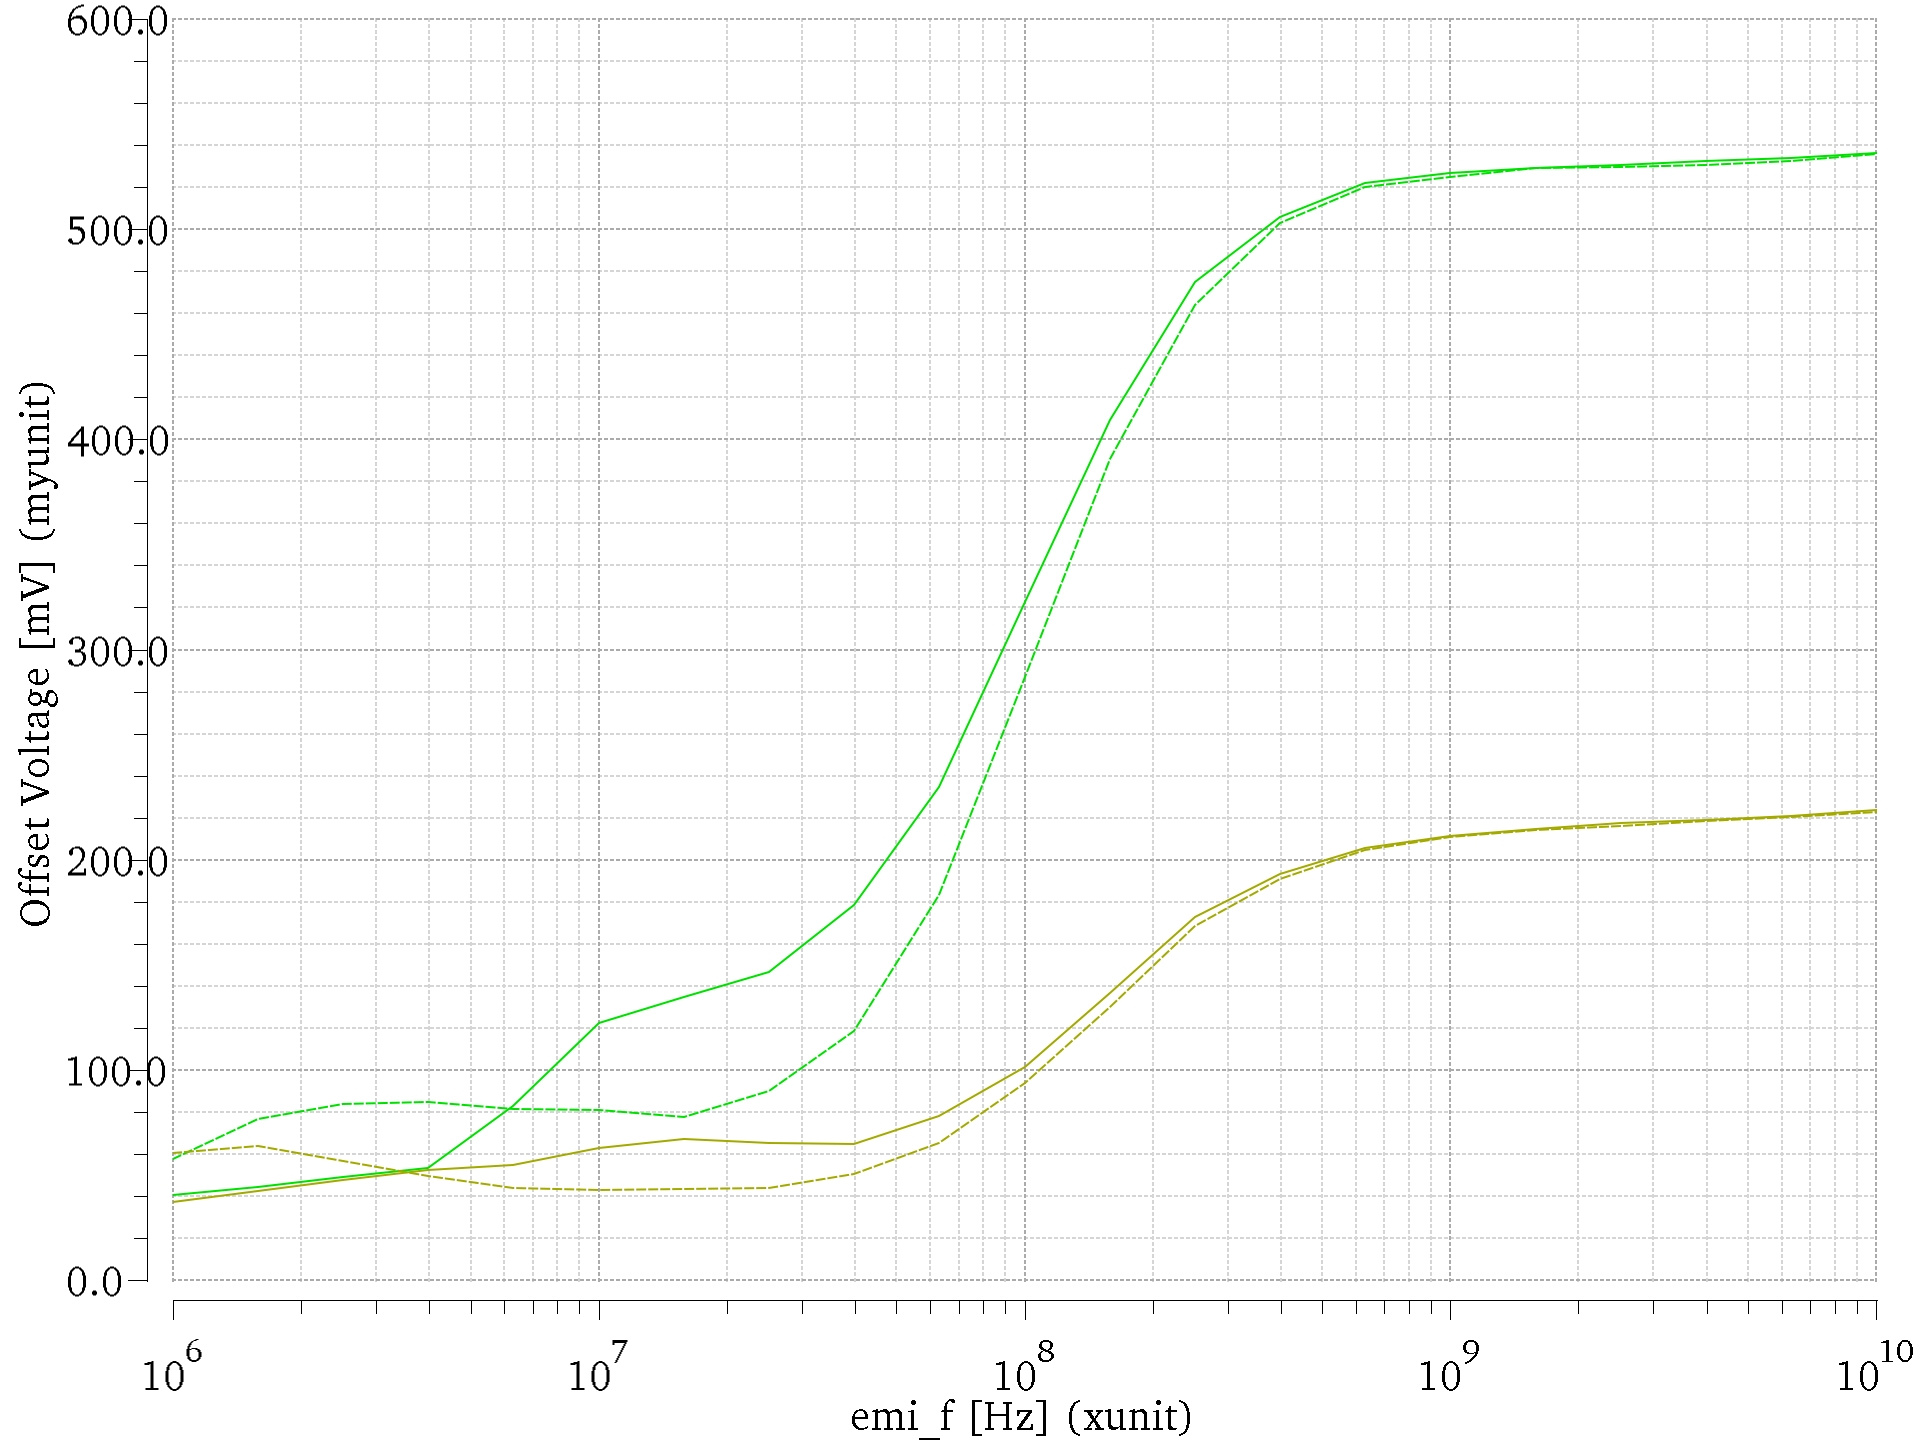
\includegraphics[width=\textwidth]{img/miller/single/emi_comparison.jpg}
    \vspace{0.2cm}
    \small
    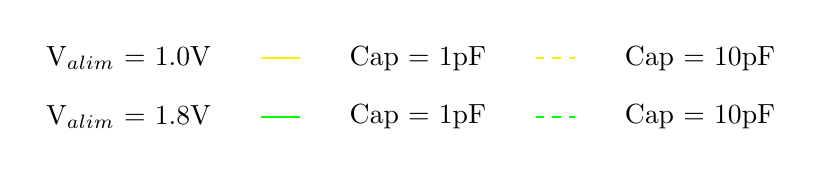
\begin{tikzpicture}
        \matrix[column sep=0.5cm, row sep=0.2cm] {
            \node[right]{V$_{alim}$ = 1.0V}; &
            \draw[yellow, thick] (0,0) -- (0.5,0); & \node{Cap = 1pF}; &
            \draw[yellow, thick, dashed] (0,0) -- (0.5,0); & \node{Cap = 10pF}; \\
            \node[right]{V$_{alim}$ = 1.8V}; &
            \draw[green, thick] (0,0) -- (0.5,0); & \node{Cap = 1pF}; &
            \draw[green, thick, dashed] (0,0) -- (0.5,0); & \node{Cap = 10pF}; \\
        };
    \end{tikzpicture}
    \caption{Risultati delle simulazioni per l'emi rejection dell'OTA di Miller a stadio singolo.}
    \label{fig:results_miller_single_stage_emi_rejection}
\end{figure}

\section{Analisi dei risultati per l'OTA di Nauta a stadio doppio}
\label{sec:results_ota_nauta_double_stage}
\subsubsection{Schematico di riferimento per la simulazione}
\label{sec:results_ota_nauta_double_stage_reference_schematic}
Lo schematico di riferimento per l'OTA di Nauta a stadio doppio è mostrato nella figura \ref{fig:schematic_nauta_double_stage}. Anche in questo caso, la capacità di carico è di 1pF.
\begin{figure}[H]
    \centering
    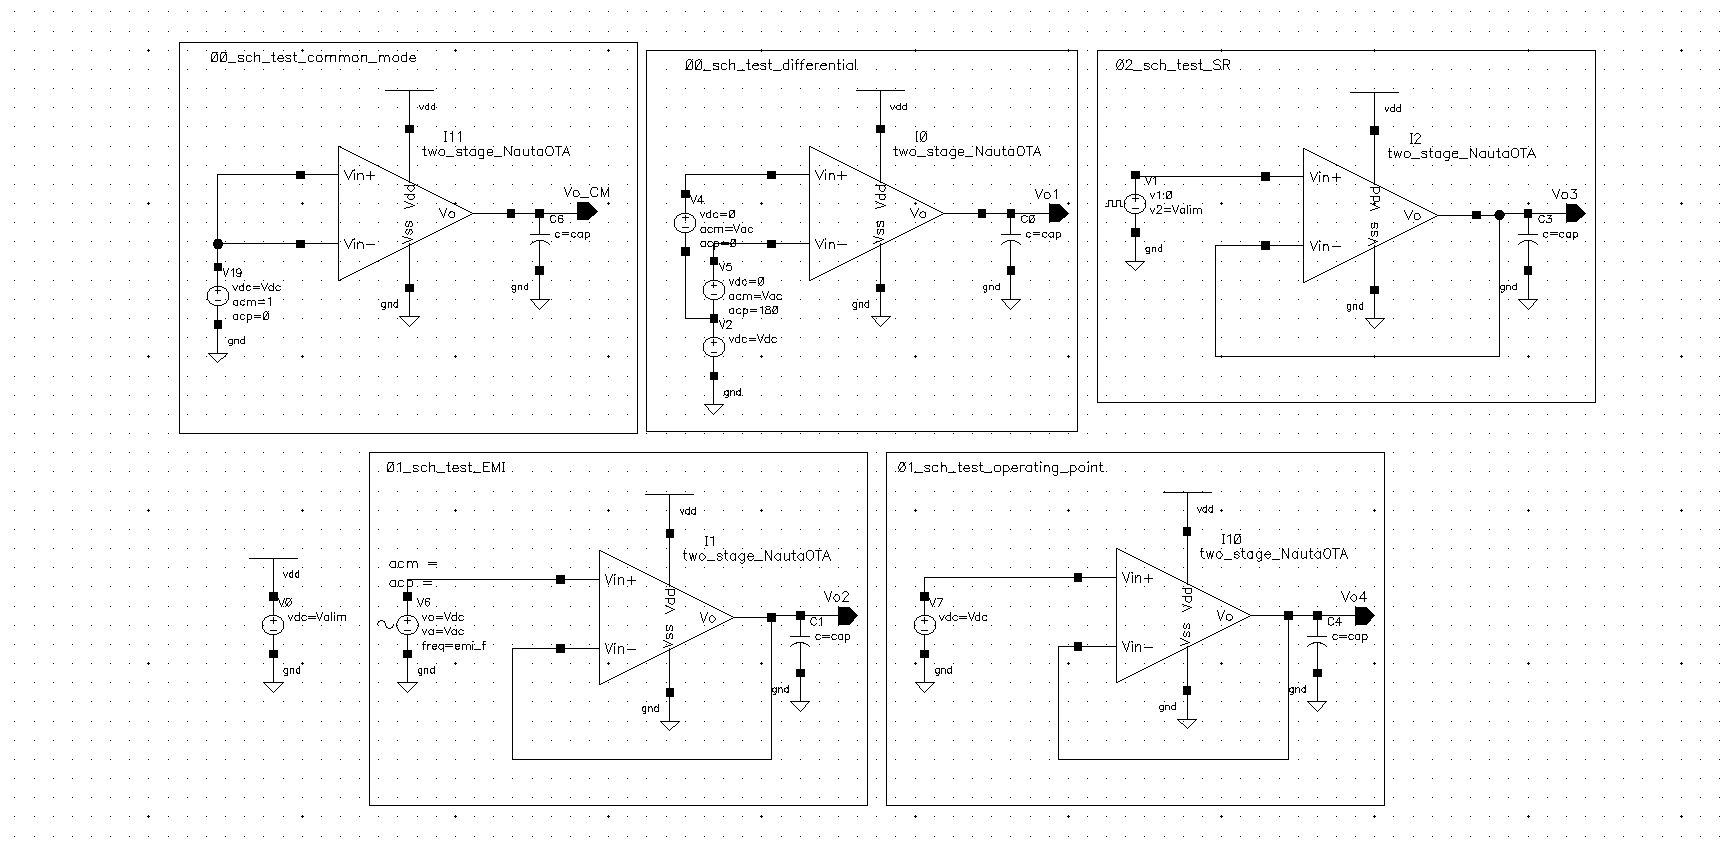
\includegraphics[width=\textwidth]{img/nauta/double/sim_nauta_double.png}
    \caption{Schematico di riferimento per l'OTA di Nauta a stadio doppio.}
    \label{fig:schematic_nauta_double_stage}
\end{figure}

Il blocco \textit{two\_stage\_NautaOTA} dell'OTA di Nauta a stadio doppio viene riportato nella figura \ref{fig:schematic_nauta_double_stage_inverter}.

\begin{figure}[H]
    \centering
    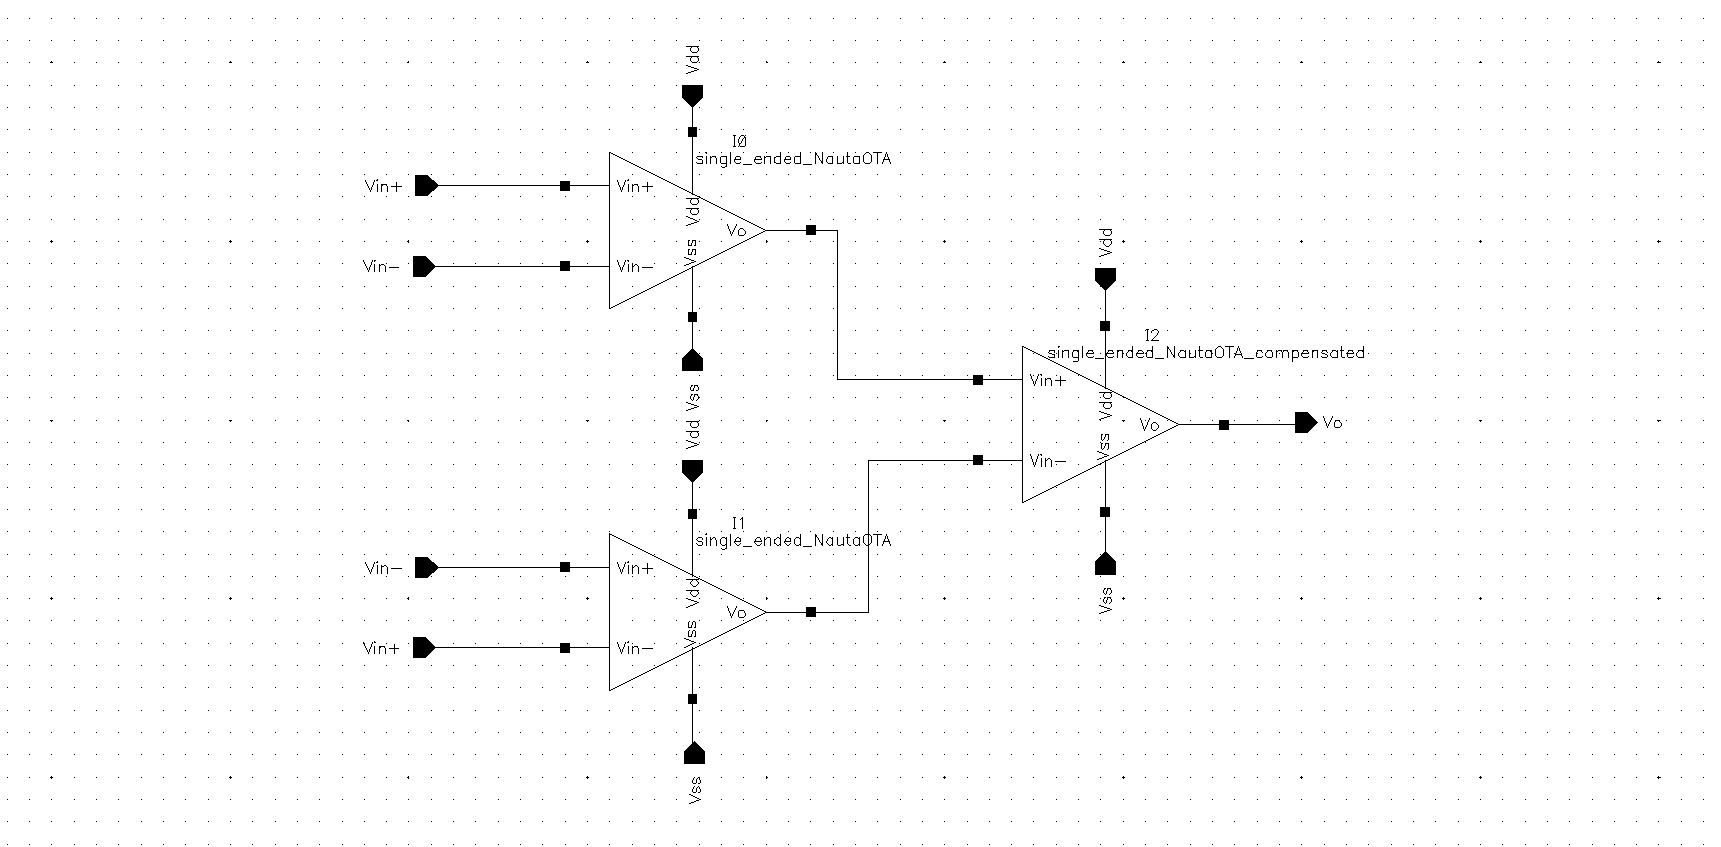
\includegraphics[width=\textwidth]{img/nauta/double/sch_nauta_double.png}
    \caption{Schematico di riferimento per il blocco \textit{two\_stage\_NautaOTA} dell'OTA di Nauta a stadio doppio.}
    \label{fig:schematic_nauta_double_stage_inverter}
\end{figure}

I blocchi \textit{OTA\_Nauta\_compensated} sono mostrati nella figura \ref{fig:schematic_nauta_double_stage_compensated}.

\begin{figure}[H]
    \centering
    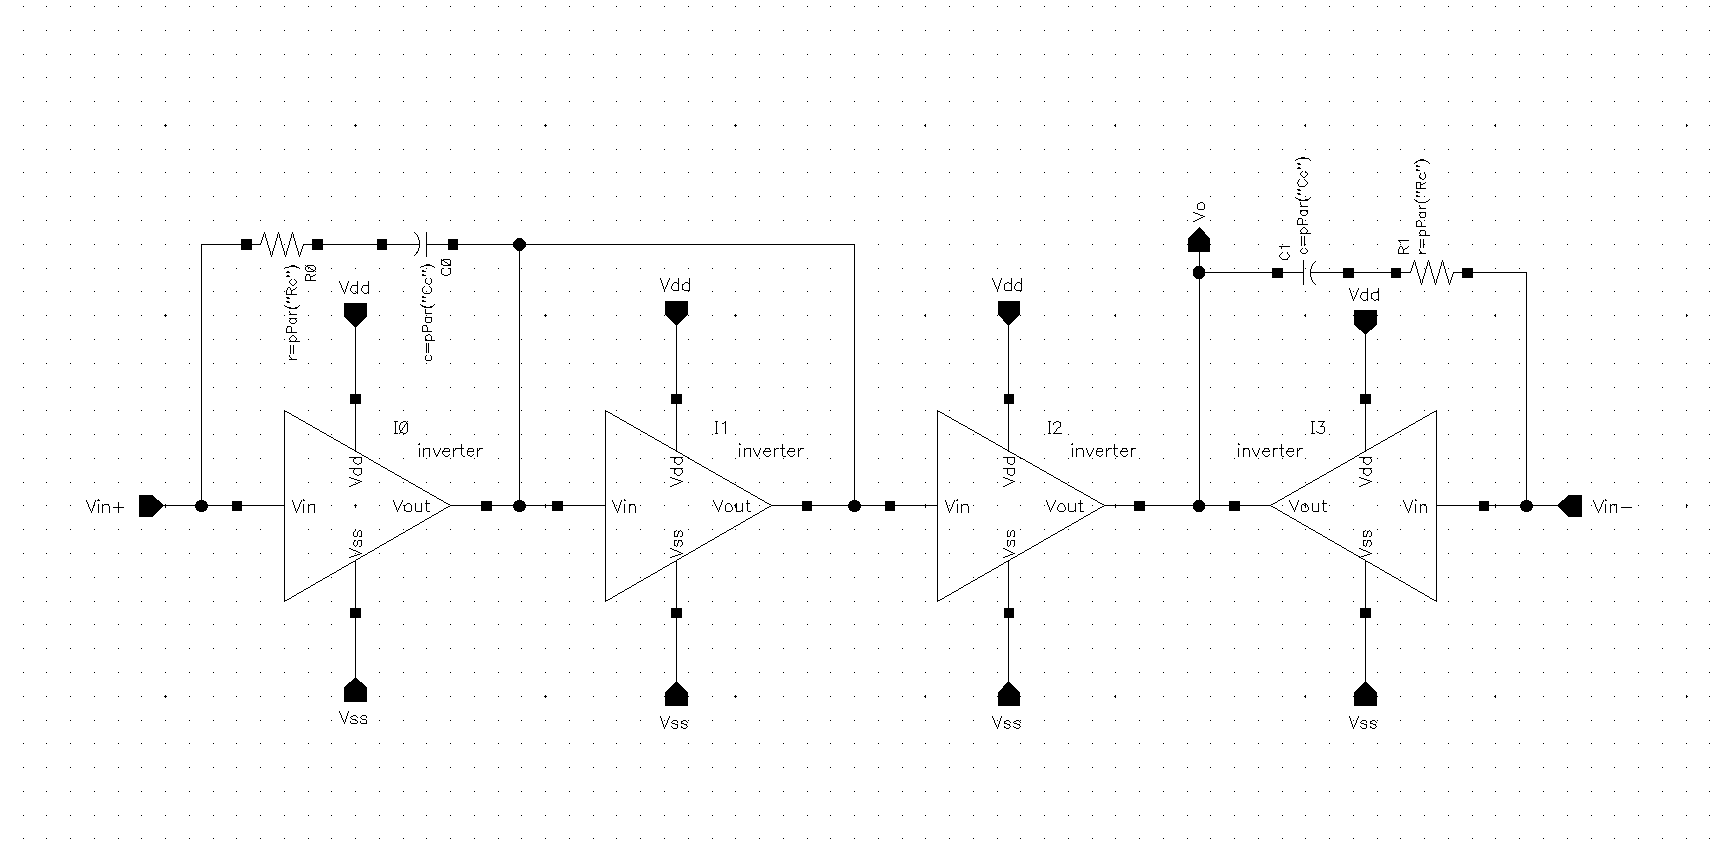
\includegraphics[width=\textwidth]{img/nauta/double/sch_nauta_ota_compensated.png}
    \caption{Schematico di riferimento per il blocco \textit{OTA\_Nauta\_compensated} dell'OTA di Nauta a stadio doppio.}
    \label{fig:schematic_nauta_double_stage_compensated}
\end{figure}

Infine, al loro interno nei blocchi \textit{Inverter} sono presenti gli inverter, che sono gli stessi utilizzati per l'OTA di Nauta a stadio singolo. La figura \ref{fig:schematic_nauta_double_stage_inverter} mostra lo schematico di riferimento per la cella inverter base, che è composta da un transistor NMOS e un transistor PMOS.

\begin{figure}[H]
    \centering
    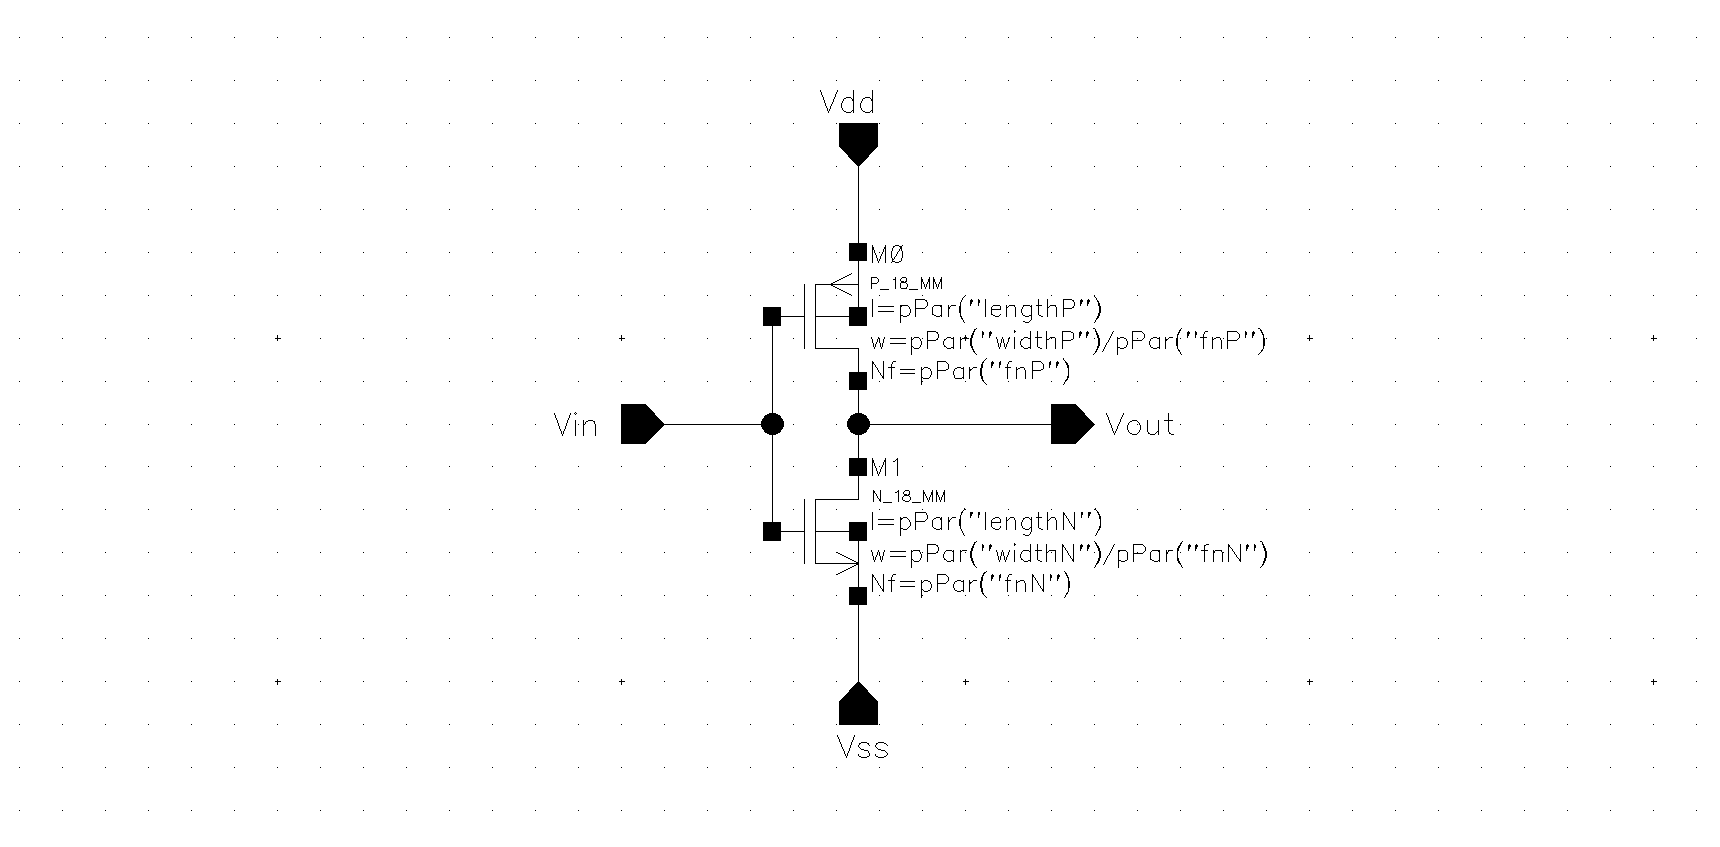
\includegraphics[width=\textwidth]{img/nauta/double/sch_inverter.png}
    \caption{Schematico di riferimento per la cella inverter base.}
    \label{fig:schematic_nauta_double_stage_inverter}
\end{figure}

\subsubsection{Dimensionamento dei componenti}
\label{sec:results_ota_nauta_double_stage_component_sizing}
I parametri di dimensionamento sono stati scelti in modo da garantire un guadagno di tensione intorno a 80 dB e un margine di fase di almeno 60°. I valori di dimensionamento scelti e i relativi risultati sono riportati nella Tabella \ref{tab:component_sizing_nauta_double_stage}.


\begin{longtable}{c|c|c|c|}
    \caption{Dimensionamento dei componenti dell'OTA di Nauta a stadio doppio. Tutti i risultati sono stati ottenuti con una capacità di carico di 1pF.}
    \label{tab:component_sizing_nauta_double_stage} \\
    
    \cline{2-4}
    & \textbf{Valim = 0.5V} & \textbf{Valim = 1V} & \textbf{Valim = 1.8V} \\ \hline
    \multicolumn{4}{|c|}{\textbf{Parametri di simulazione}} \\ \hline
    \endfirsthead
    
    \multicolumn{4}{c}{\tablename\ \thetable{} -- Continua dalla pagina precedente} \\
    \cline{2-4}
    & \textbf{Valim = 0.5V} & \textbf{Valim = 1V} & \textbf{Valim = 1.8V} \\ \hline
    \endhead
    
    \multicolumn{4}{r}{{Continua nella pagina successiva}} \\
    \endfoot
    
    \endlastfoot

    \multicolumn{1}{|c|}{Cc} & 10pF & 6pF & 5pF \\ \hline
    \multicolumn{1}{|c|}{LN} & 1$\mu$m & 1$\mu$m & 1$\mu$m \\ \hline
    \multicolumn{1}{|c|}{Rc} & 10k$\Omega$ & 4k$\Omega$ & 1k$\Omega$ \\ \hline
    \multicolumn{1}{|c|}{WN} & 12$\mu$m & 6$\mu$m & 6$\mu$m \\ \hline
    \multicolumn{1}{|c|}{fnN} & 6 & 2 & 2 \\ \hline
    \multicolumn{1}{|c|}{fnP} & 2*fnN & fnP & 2*fnN \\ \hline
    \multicolumn{1}{|c|}{LP} & LN & LN & LN \\ \hline
    \multicolumn{1}{|c|}{WP} & 2*WN & 4*WN & 4*WN \\ \hline
    \multicolumn{1}{|c|}{Vac} & Valim/2 & Valim/2 & Valim/2 \\ \hline
    \multicolumn{1}{|c|}{Vdc} & Valim/2 & Valim/2 & Valim/2 \\ \hline
    \multicolumn{1}{|c|}{fnN2} & fnN & fnN & fnN \\ \hline
    \multicolumn{1}{|c|}{lengthN2} & 2*LN & 2*LN & 2*LN \\ \hline
    \multicolumn{1}{|c|}{widthN2} & 4*WN & 3*WN & 3*WN \\ \hline
    \multicolumn{1}{|c|}{fnP2} & fnP & fnP & fnP \\ \hline
    \multicolumn{1}{|c|}{lengthP2} & 2*LP & 2*LP & 2*LP \\ \hline
    \multicolumn{1}{|c|}{widthP2} & 4*WP & 2*WP & 2*WP \\ \hline
    \multicolumn{4}{|c|}{\textbf{Risultati simulazione}} \\ \hline
    \multicolumn{1}{|c|}{I0/I0/M0 region} & 3 & 2 & 2 \\ \hline
    \multicolumn{1}{|c|}{I0/I0/M1 region} & 3 & 2 & 2 \\ \hline
    \multicolumn{1}{|c|}{I0/I1/M0 region} & 3 & 2 & 2 \\ \hline
    \multicolumn{1}{|c|}{I0/I1/M1 region} & 3 & 2 & 2 \\ \hline
    \multicolumn{1}{|c|}{I0/I2/M0 region} & 3 & 2 & 2 \\ \hline
    \multicolumn{1}{|c|}{I0/I2/M1 region} & 3 & 2 & 2 \\ \hline
    \multicolumn{1}{|c|}{I0/I3/M0 region} & 3 & 2 & 2 \\ \hline
    \multicolumn{1}{|c|}{I0/I3/M1 region} & 3 & 2 & 2 \\ \hline
    \multicolumn{1}{|c|}{I0/I4/M0 region} & 3 & 2 & 2 \\ \hline
    \multicolumn{1}{|c|}{I0/I4/M1 region} & 3 & 2 & 2 \\ \hline
    \multicolumn{1}{|c|}{I1/I0/M0 region} & 3 & 2 & 2 \\ \hline
    \multicolumn{1}{|c|}{I1/I0/M1 region} & 3 & 2 & 2 \\ \hline
    \multicolumn{1}{|c|}{I1/I1/M0 region} & 3 & 2 & 2 \\ \hline
    \multicolumn{1}{|c|}{I1/I1/M1 region} & 3 & 2 & 2 \\ \hline
    \multicolumn{1}{|c|}{I1/I2/M0 region} & 3 & 2 & 2 \\ \hline
    \multicolumn{1}{|c|}{I1/I2/M1 region} & 3 & 2 & 2 \\ \hline
    \multicolumn{1}{|c|}{I1/I3/M0 region} & 3 & 2 & 2 \\ \hline
    \multicolumn{1}{|c|}{I1/I3/M1 region} & 3 & 2 & 2 \\ \hline
    \multicolumn{1}{|c|}{I1/I4/M0 region} & 3 & 2 & 2 \\ \hline
    \multicolumn{1}{|c|}{I1/I4/M1 region} & 3 & 2 & 2 \\ \hline
    \multicolumn{1}{|c|}{I2/I0/M0 region} & 3 & 2 & 2 \\ \hline
    \multicolumn{1}{|c|}{I2/I0/M1 region} & 3 & 2 & 2 \\ \hline
    \multicolumn{1}{|c|}{I2/I1/M0 region} & 3 & 2 & 2 \\ \hline
    \multicolumn{1}{|c|}{I2/I1/M1 region} & 3 & 2 & 2 \\ \hline
    \multicolumn{1}{|c|}{I2/I2/M0 region} & 3 & 2 & 2 \\ \hline
    \multicolumn{1}{|c|}{I2/I2/M1 region} & 3 & 2 & 2 \\ \hline
    \multicolumn{1}{|c|}{I2/I3/M0 region} & 3 & 2 & 2 \\ \hline
    \multicolumn{1}{|c|}{I2/I3/M1 region} & 3 & 2 & 2 \\ \hline
    \multicolumn{1}{|c|}{I2/I4/M0 region} & 3 & 2 & 2 \\ \hline
    \multicolumn{1}{|c|}{I2/I4/M1 region} & 3 & 2 & 2 \\ \hline
    \multicolumn{1}{|c|}{AV(0)} & 72.51dB & 79.68dB & 75.87dB \\ \hline
    \multicolumn{1}{|c|}{f$_c$} & 13.98Hz & 1.136kHz & 13.68kHz \\ \hline
    \multicolumn{1}{|c|}{f$_o$} & 70.32kHz & 8.312MHz & 104.8MHz \\ \hline
\end{longtable}

\subsubsection{A$_v$, Phase, CMRR e CMR}   
\label{sec:results_ota_nauta_double_stage_A_V_phase}
Di seguito vengono riportati i risultati delle simulazioni per il guadagno di tensione ($A_V$) e la fase (Phase) dell'OTA di Nauta a stadio doppio.

\begin{figure}[H]
    \centering
    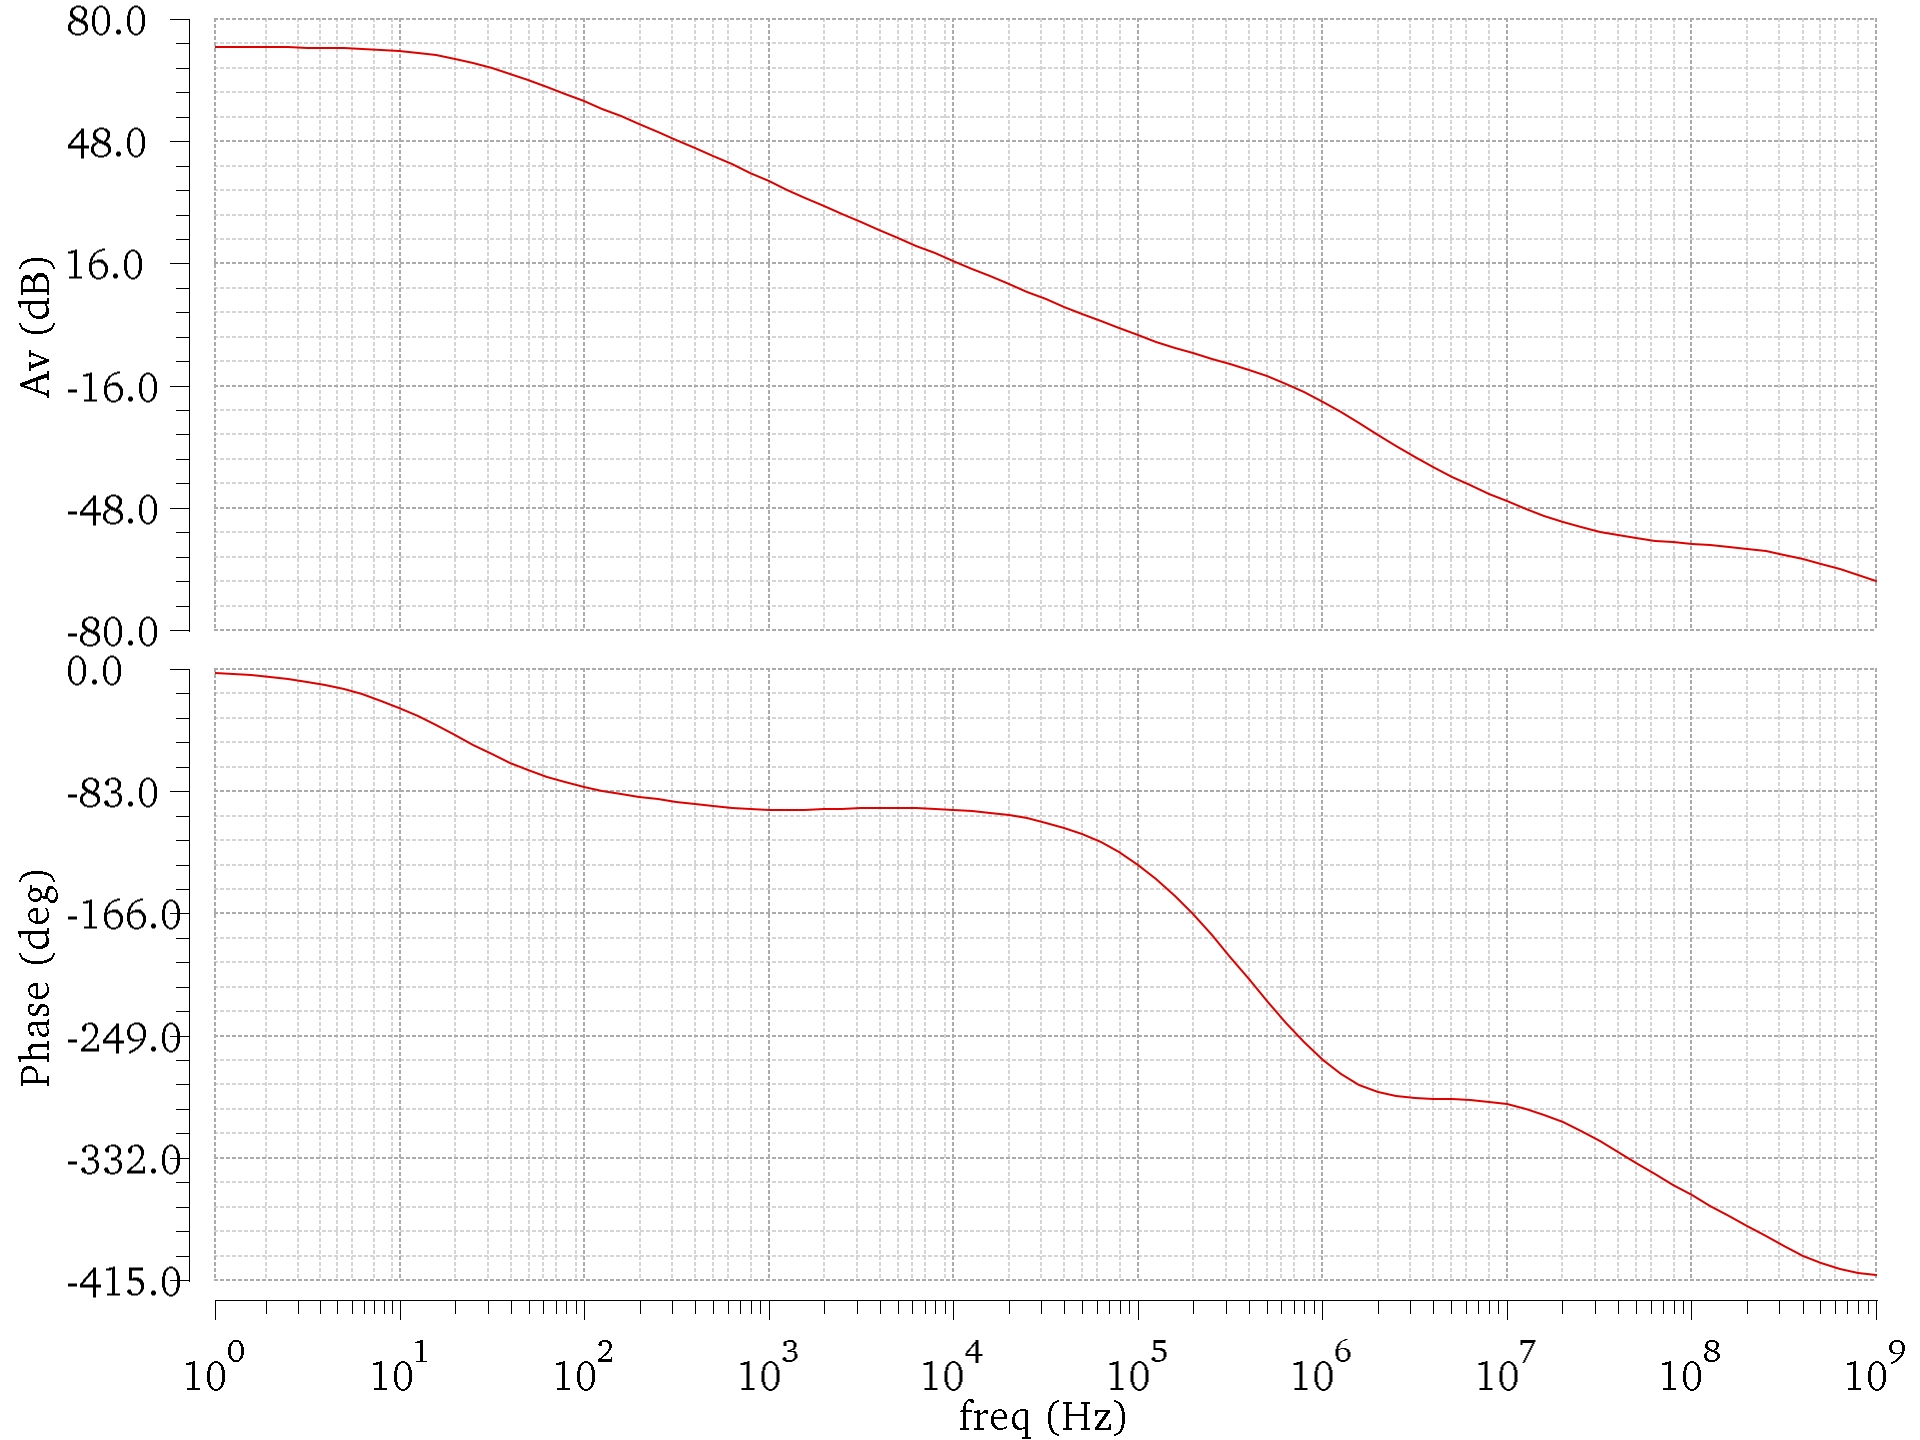
\includegraphics[width=\textwidth]{img/nauta/double/av_ph_0_5V.jpg}
    \caption{Risultati delle simulazioni per il guadagno di tensione ($A_V$) e la fase (Phase) dell'OTA di Nauta a stadio doppio con Valim = 0.5V.}    
    \label{fig:results_nauta_double_stage_A_V_phase_0_5V}
\end{figure}

\begin{figure}[H]
    \centering
    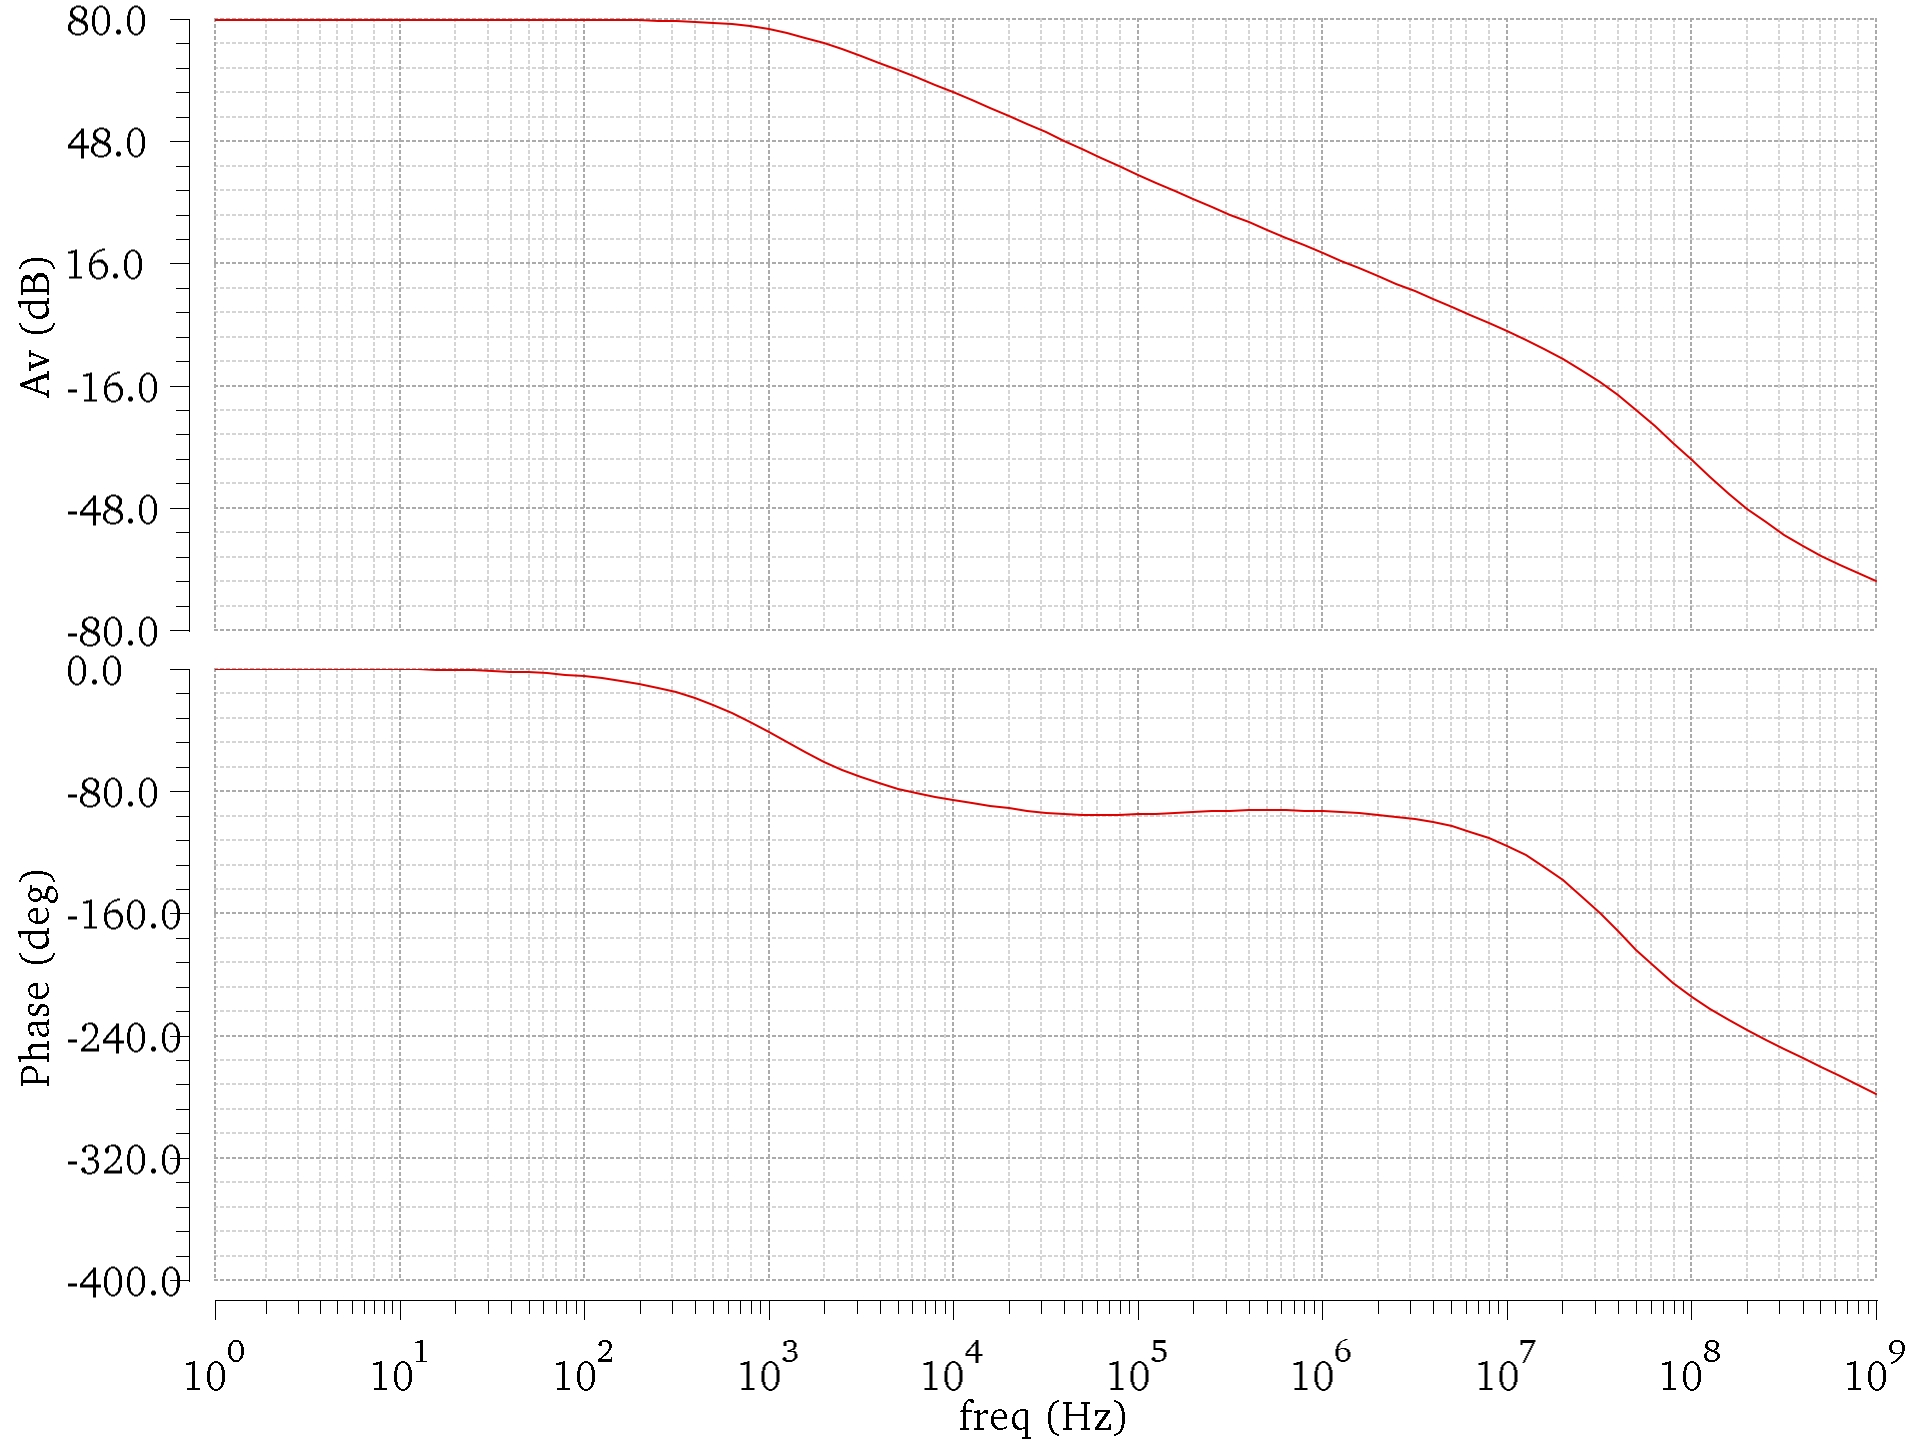
\includegraphics[width=\textwidth]{img/nauta/double/av_ph_1V.jpg}
    \caption{Risultati delle simulazioni per il guadagno di tensione ($A_V$) e la fase (Phase) dell'OTA di Nauta a stadio doppio con Valim = 1V.}
    \label{fig:results_nauta_double_stage_A_V_phase_1V}
\end{figure}

\begin{figure}[H]
    \centering
    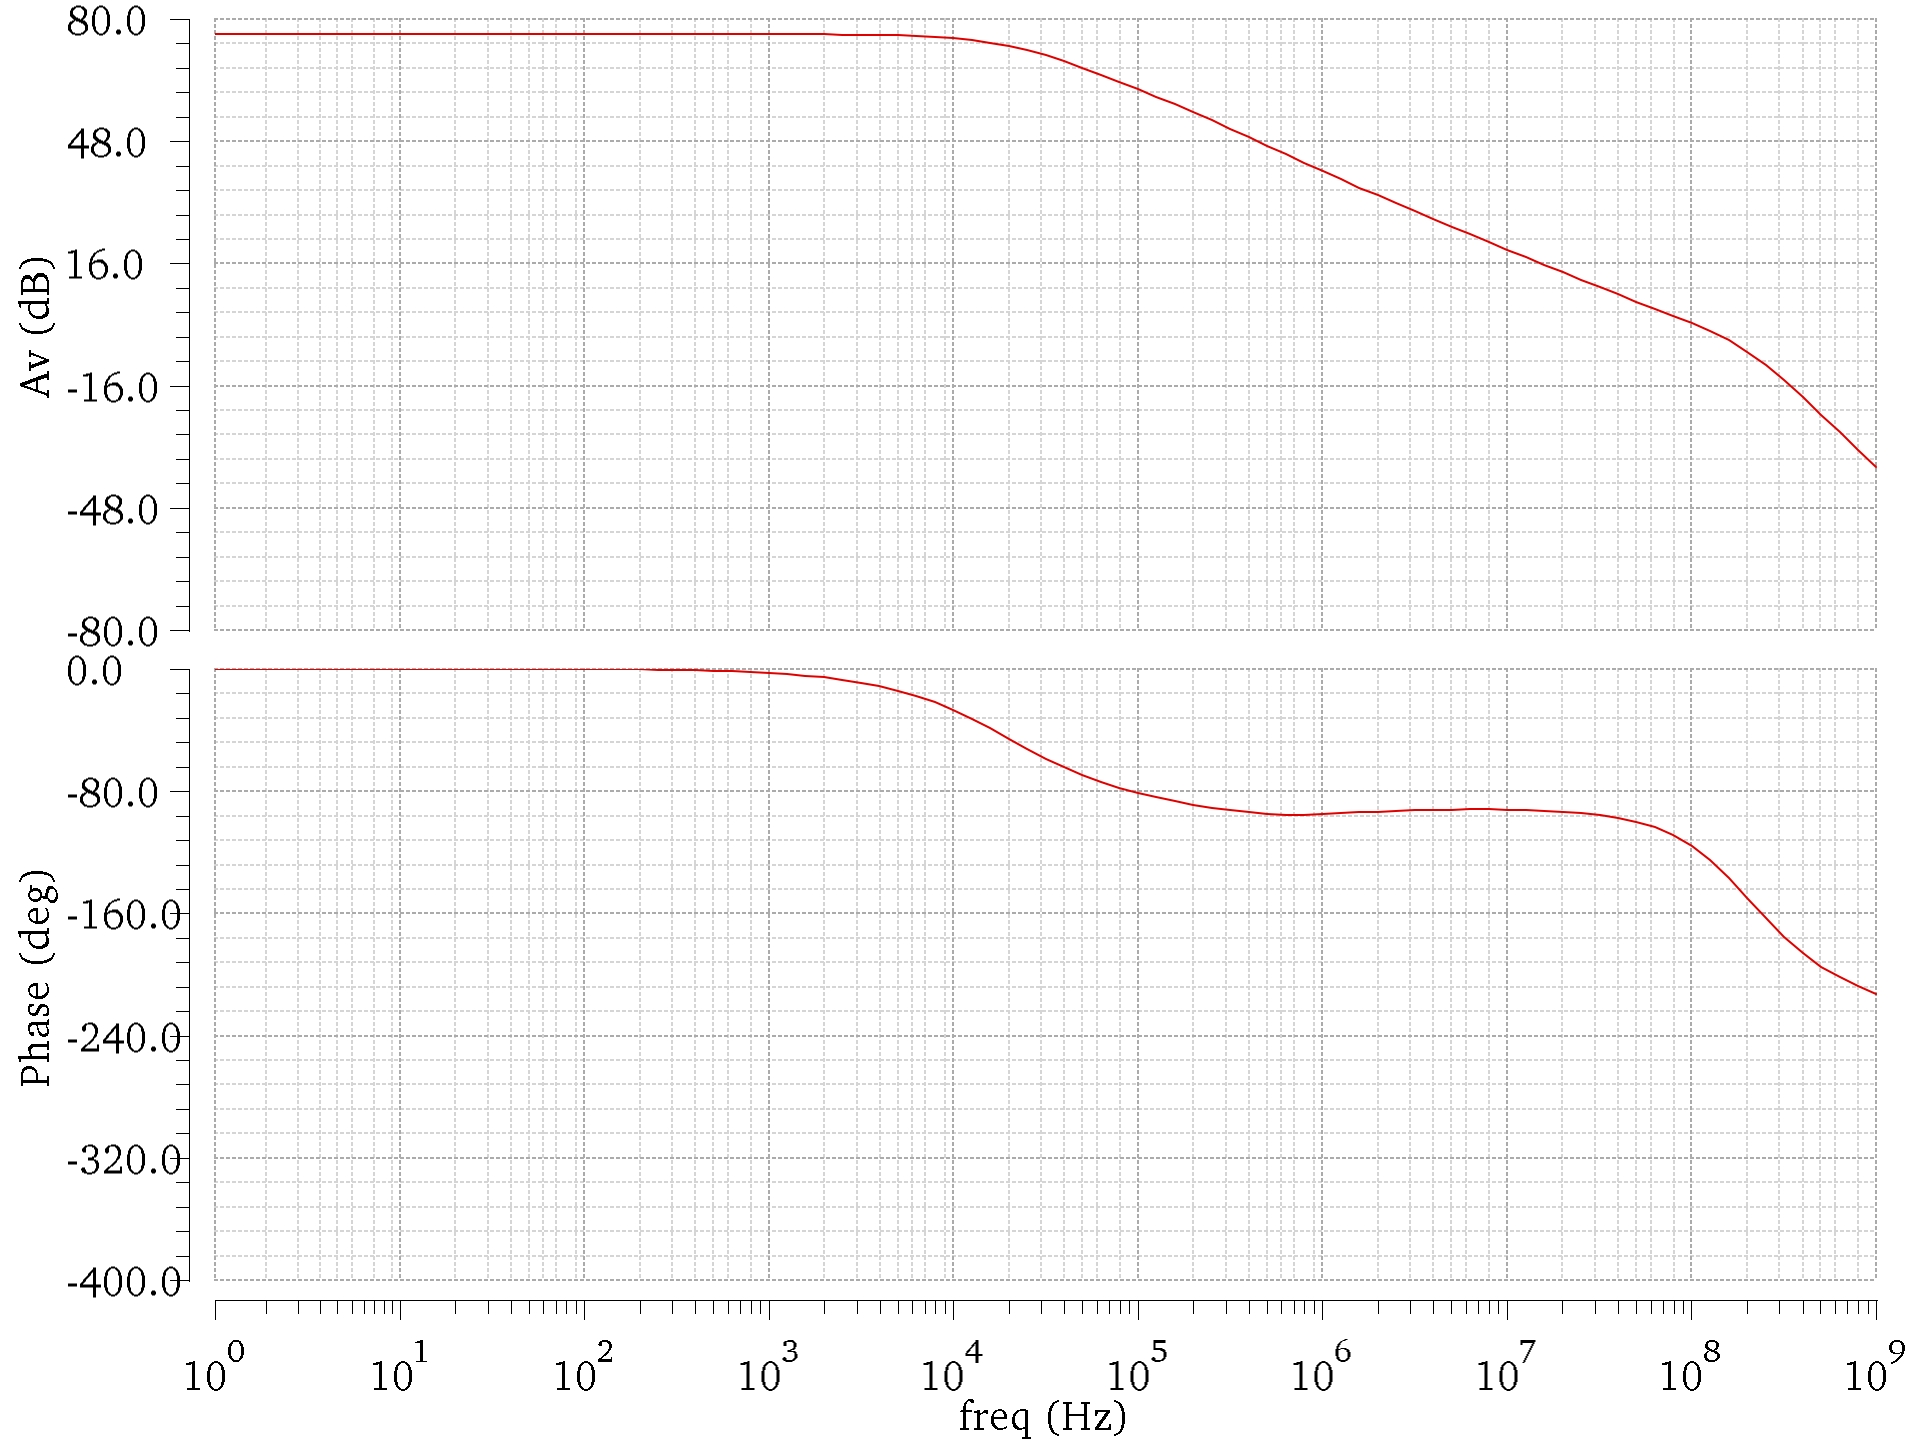
\includegraphics[width=\textwidth]{img/nauta/double/av_ph_1_8V.jpg}
    \caption{Risultati delle simulazioni per il guadagno di tensione ($A_V$) e la fase (Phase) dell'OTA di Nauta a stadio doppio con Valim = 1.8V.}
    \label{fig:results_nauta_double_stage_A_V_phase_1_8V}
\end{figure}

Di seguito vengono riportati i risultati delle simulazioni per il rapporto di reiezione al modo comume (CMRR) e il range di modo comune (CMR) dell'OTA di Nauta a stadio doppio.
\begin{figure}[H]
    \centering
    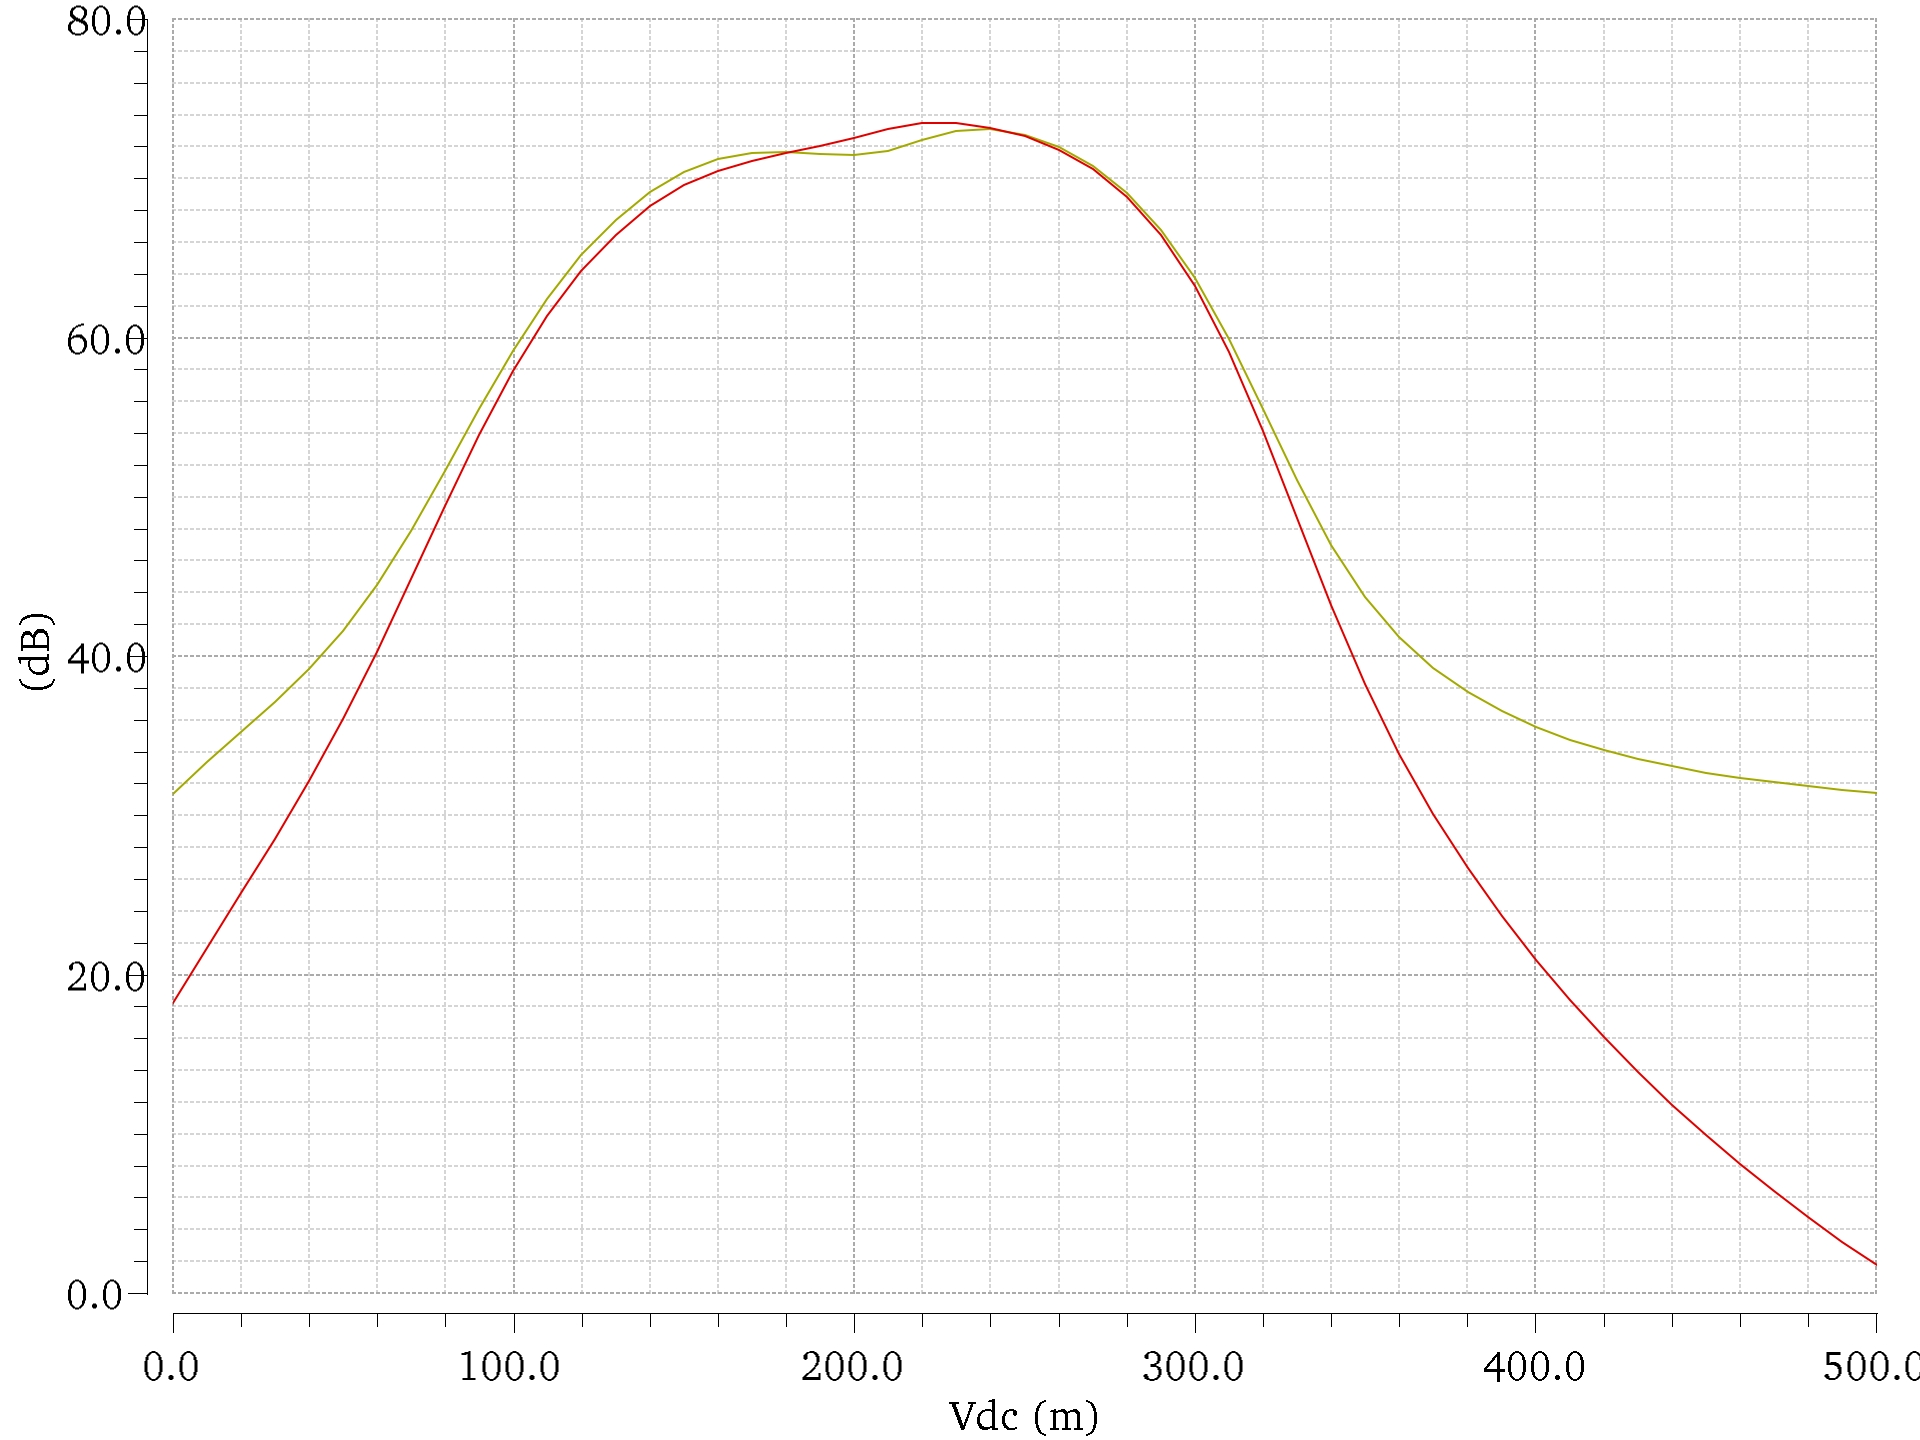
\includegraphics[width=\textwidth]{img/nauta/double/cmr_cmrr_0_5V.jpg}
    \vspace{0.2cm}
    \small
    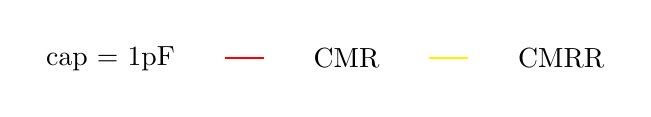
\begin{tikzpicture}
        \matrix[column sep=0.5cm, row sep=0.2cm] {
            \node[right]{cap = 1pF}; &
            \draw[red, thick] (0,0) -- (0.5,0); & \node{CMR}; &
            \draw[yellow, thick] (0,0) -- (0.5,0); & \node{CMRR}; \\
        };
    \end{tikzpicture}
    \caption{Risultati delle simulazioni per il rapporto di reiezione al modo comume (CMRR) e il range di modo comune (CMR) dell'OTA di Nauta a stadio doppio con Valim = 0.5V.}
    \label{fig:results_nauta_double_stage_CMRR_CMR_0_5V}
\end{figure}

\begin{figure}[H]
    \centering
    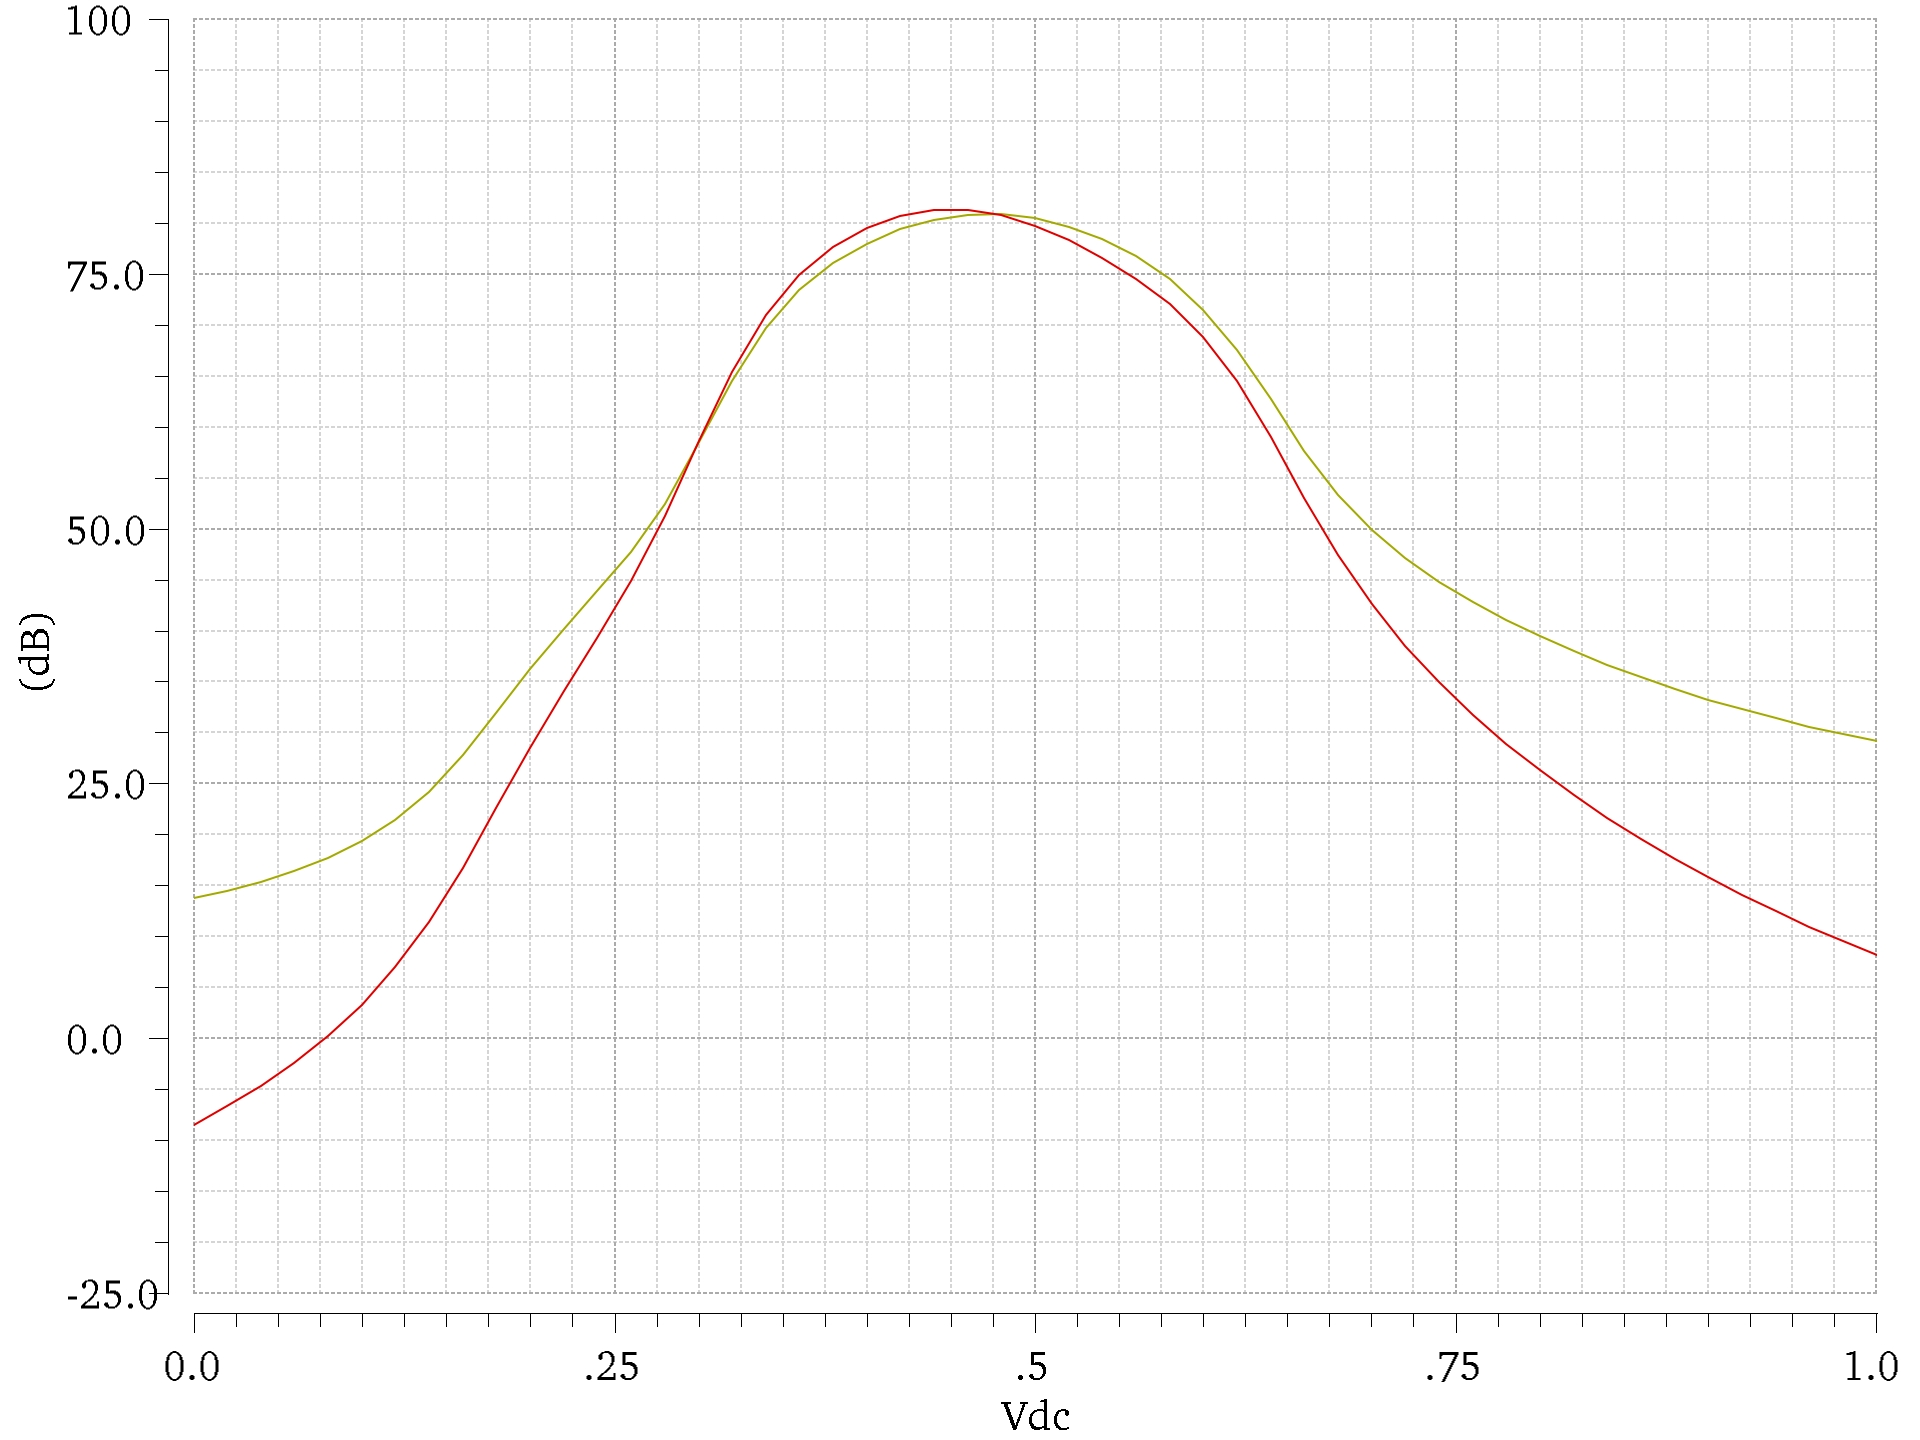
\includegraphics[width=\textwidth]{img/nauta/double/cmr_cmrr_1V.jpg}
    \vspace{0.2cm}
    \small
    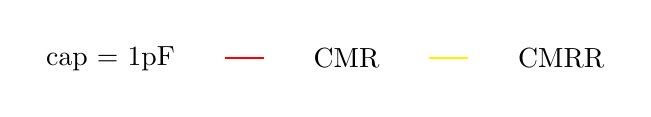
\begin{tikzpicture}
        \matrix[column sep=0.5cm, row sep=0.2cm] {
            \node[right]{cap = 1pF}; &
            \draw[red, thick] (0,0) -- (0.5,0); & \node{CMR}; &
            \draw[yellow, thick] (0,0) -- (0.5,0); & \node{CMRR}; \\
        };
    \end{tikzpicture}
    \caption{Risultati delle simulazioni per il rapporto di reiezione al modo comume (CMRR) e il range di modo comune (CMR) dell'OTA di Nauta a stadio doppio con Valim = 1V.}
    \label{fig:results_nauta_double_stage_CMRR_CMR_1V}
\end{figure}

\begin{figure}[H]
    \centering
    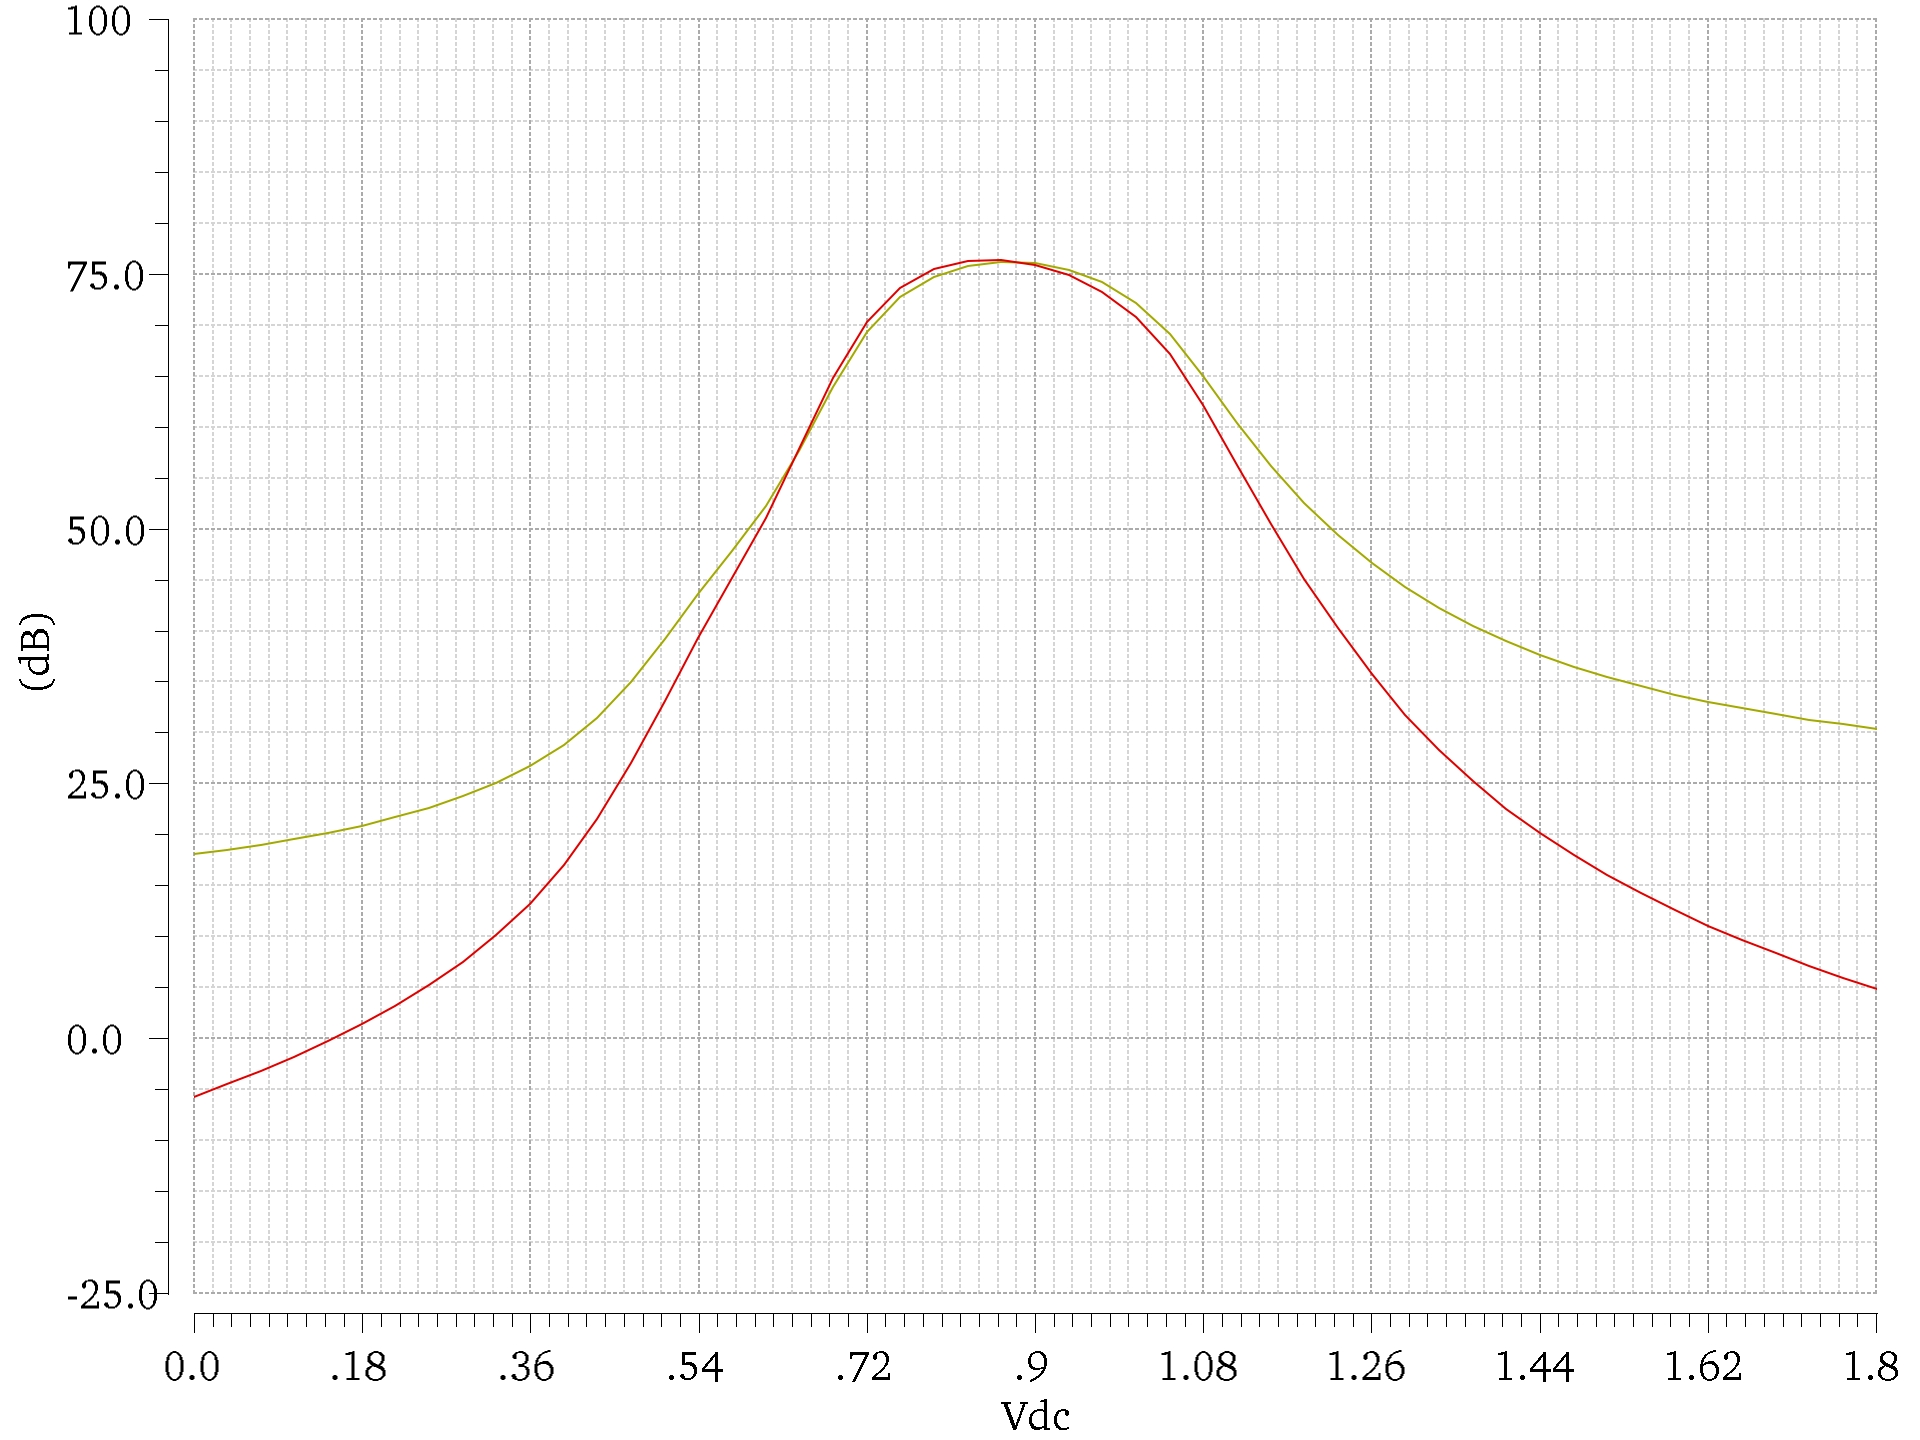
\includegraphics[width=\textwidth]{img/nauta/double/cmr_cmrr_1_8V.jpg}
    \vspace{0.2cm}
    \small
    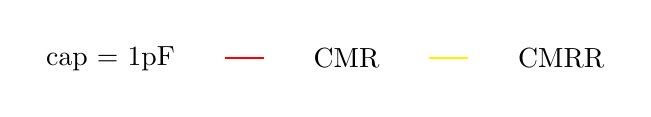
\begin{tikzpicture}
        \matrix[column sep=0.5cm, row sep=0.2cm] {
            \node[right]{cap = 1pF}; &
            \draw[red, thick] (0,0) -- (0.5,0); & \node{CMR}; &
            \draw[yellow, thick] (0,0) -- (0.5,0); & \node{CMRR}; \\
        };
    \end{tikzpicture}
    \caption{Risultati delle simulazioni per il rapporto di reiezione al modo comume (CMRR) e il range di modo comune (CMR) dell'OTA di Nauta a stadio doppio con Valim = 1.8V.}
    \label{fig:results_nauta_double_stage_CMRR_CMR_1_8V}
\end{figure}

Come si può notare dalle figure \ref{fig:results_nauta_double_stage_CMRR_CMR_0_5V}, \ref{fig:results_nauta_double_stage_CMRR_CMR_1V} e \ref{fig:results_nauta_double_stage_CMRR_CMR_1_8V}, il CMR di questa configurazione è relativamente scarso, presentando un attenuazione del 50\% per tensioni di modo comune superiori distanti dalla metà dinamica. Inoltre questo dato peggiora all'aumentare della tensione di alimentazione.

\subsubsection{Phase Margin, Gain Bandwidth Product e Slew Rate}
\label{sec:results_ota_nauta_double_stage_phase_margin_gain_bandwidth_product_slew_rate}

Di seguito vengono riportati i risultati delle simulazioni per il margine di fase (Phase Margin), il prodotto guadagno-banda (Gain Bandwidth Product) e lo slew rate (SR).

\begin{table}[H]
    \centering
    \caption{Risultati delle simulazioni per il margine di fase (Phase Margin), il prodotto guadagno-banda (Gain Bandwidth Product) e lo slew rate (SR) dell'OTA di Nauta a doppio stadio con capacità di carico di 1pF.}
    \begin{tabular}{|c|c|c|c|}
        \hline
        \textbf{Valim} & \textbf{Phase Margin} & \textbf{Gain Bandwidth Product} & \textbf{Slew Rate (+/-)} \\ \hline
        0.5V & 59.13° & 84.6 kHz & 1.25/1.25 V/$\mu$s \\ \hline
        1V & 68.49° & 11 MHz & 23.5/23.5 V/$\mu$s \\ \hline
        1.8V & 62.67° & 122.6 MHz & 138/138 V/$\mu$s \\ \hline
    \end{tabular}
    \label{tab:results_nauta_double_stage_1pF}
\end{table}

\begin{table}[H]
    \centering
    \caption{Risultati delle simulazioni per il margine di fase (Phase Margin), il prodotto guadagno-banda (Gain Bandwidth Product) e lo slew rate (SR) dell'OTA di Nauta a doppio stadio con capacità di carico di 10pF.}
    \begin{tabular}{|c|c|c|c|}
        \hline
        \textbf{Valim} & \textbf{Phase Margin} & \textbf{Gain Bandwidth Product} & \textbf{Slew Rate (+/-)} \\ \hline
        0.5V & 38.14° & 83.5 kHz & 0.6/0.6 V/$\mu$s \\ \hline
        1V & 33.03° & 10.8 MHz & 12/12 V/$\mu$s \\ \hline
        1.8V & 30.03° & 118.2 MHz & 70/70 V/$\mu$s \\ \hline
    \end{tabular}
    \label{tab:results_nauta_double_stage_10pF}
\end{table}

Anche qui si nota come le prestazioni del circuito con capacità di carico di 10pF siano migliori rispetto alle prestazioni del circuito con capacità di carico di 1pF.

\subsubsection{Emi rejection}
\label{sec:results_ota_nauta_double_stage_emi_rejection}
Di seguito vengono riportati i risultati delle simulazioni per l'emi rejection dell'OTA di Nauta a stadio doppio. I risultati sono stati ottenuti con una capacità di carico di 1pF.

\begin{figure}[H]
    \centering
    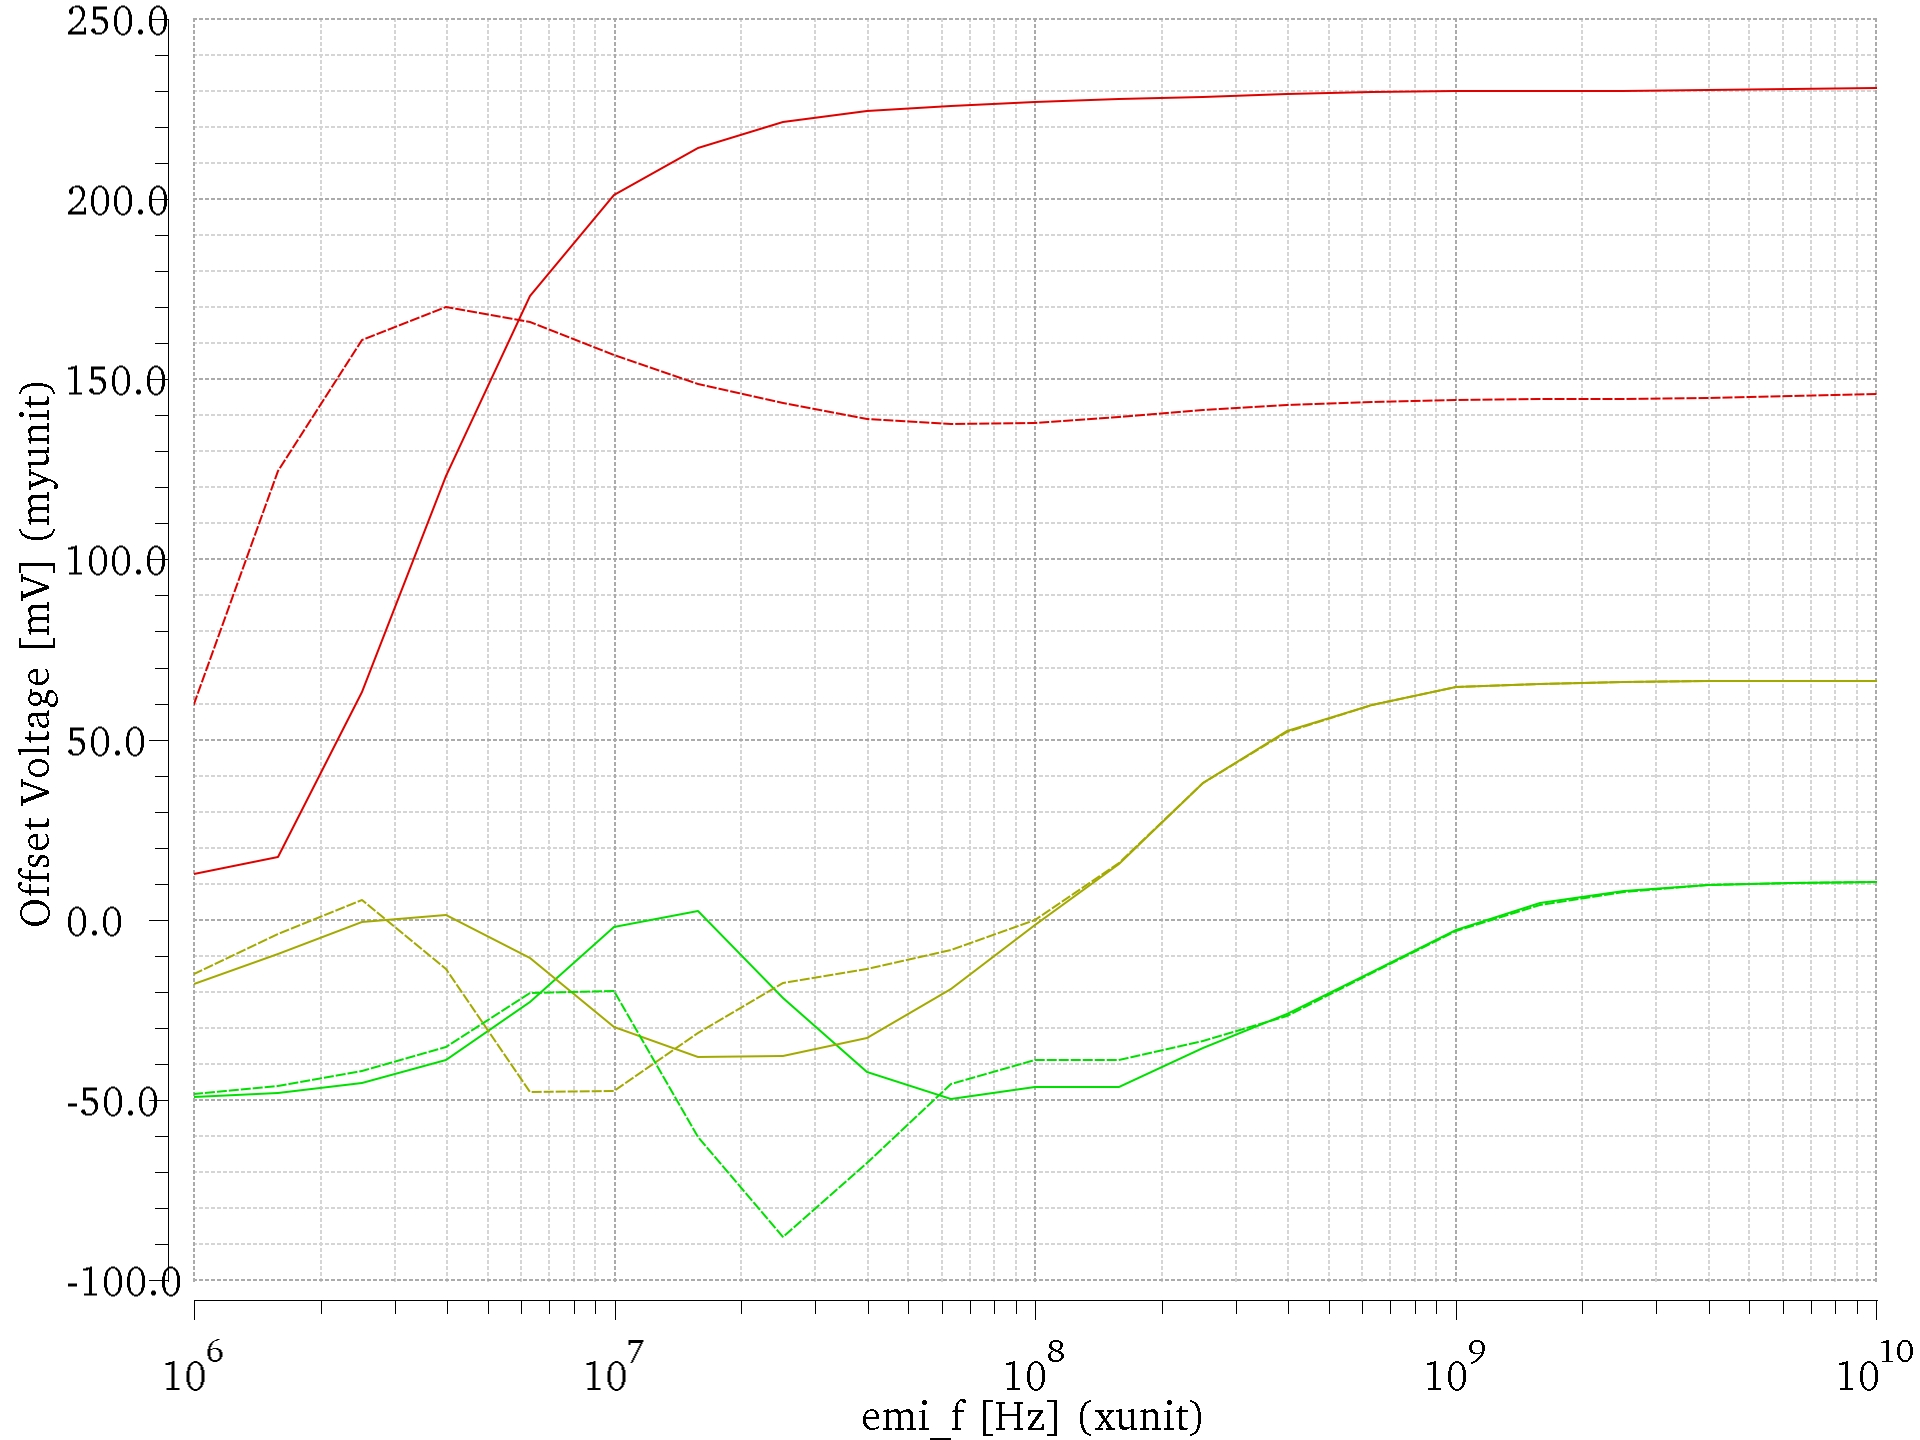
\includegraphics[width=\textwidth]{img/nauta/double/emi_comparison.jpg}
    \vspace{0.2cm}
    \small
    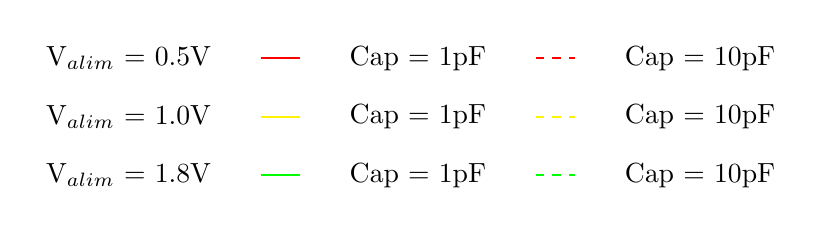
\begin{tikzpicture}
        \matrix[column sep=0.5cm, row sep=0.2cm] {
            \node[right]{V$_{alim}$ = 0.5V}; &
            \draw[red, thick] (0,0) -- (0.5,0); & \node{Cap = 1pF}; &
            \draw[red, thick, dashed] (0,0) -- (0.5,0); & \node{Cap = 10pF}; \\
            \node[right]{V$_{alim}$ = 1.0V}; &
            \draw[yellow, thick] (0,0) -- (0.5,0); & \node{Cap = 1pF}; &
            \draw[yellow, thick, dashed] (0,0) -- (0.5,0); & \node{Cap = 10pF}; \\
            \node[right]{V$_{alim}$ = 1.8V}; &
            \draw[green, thick] (0,0) -- (0.5,0); & \node{Cap = 1pF}; &
            \draw[green, thick, dashed] (0,0) -- (0.5,0); & \node{Cap = 10pF}; \\
        };
    \end{tikzpicture}
    \caption{Risultati delle simulazioni per l'emi rejection dell'OTA di Nauta a stadio doppio.}
    \label{fig:results_nauta_double_stage_emi_rejection}
\end{figure}
 

\section{Analisi dei risultati per l'OTA di Miller a stadio doppio}
\label{sec:results_ota_miller_double_stage}

\subsubsection{Schematico di riferimento per la simulazione}
\label{sec:results_ota_miller_double_stage_reference_schematic}
Lo schematico di riferimento per l'OTA di Miller a stadio doppio è mostrato nella figura \ref{fig:schematic_miller_double_stage}. Anche in questo caso, la capacità di carico è di 1pF.
\begin{figure}[H]
    \centering
    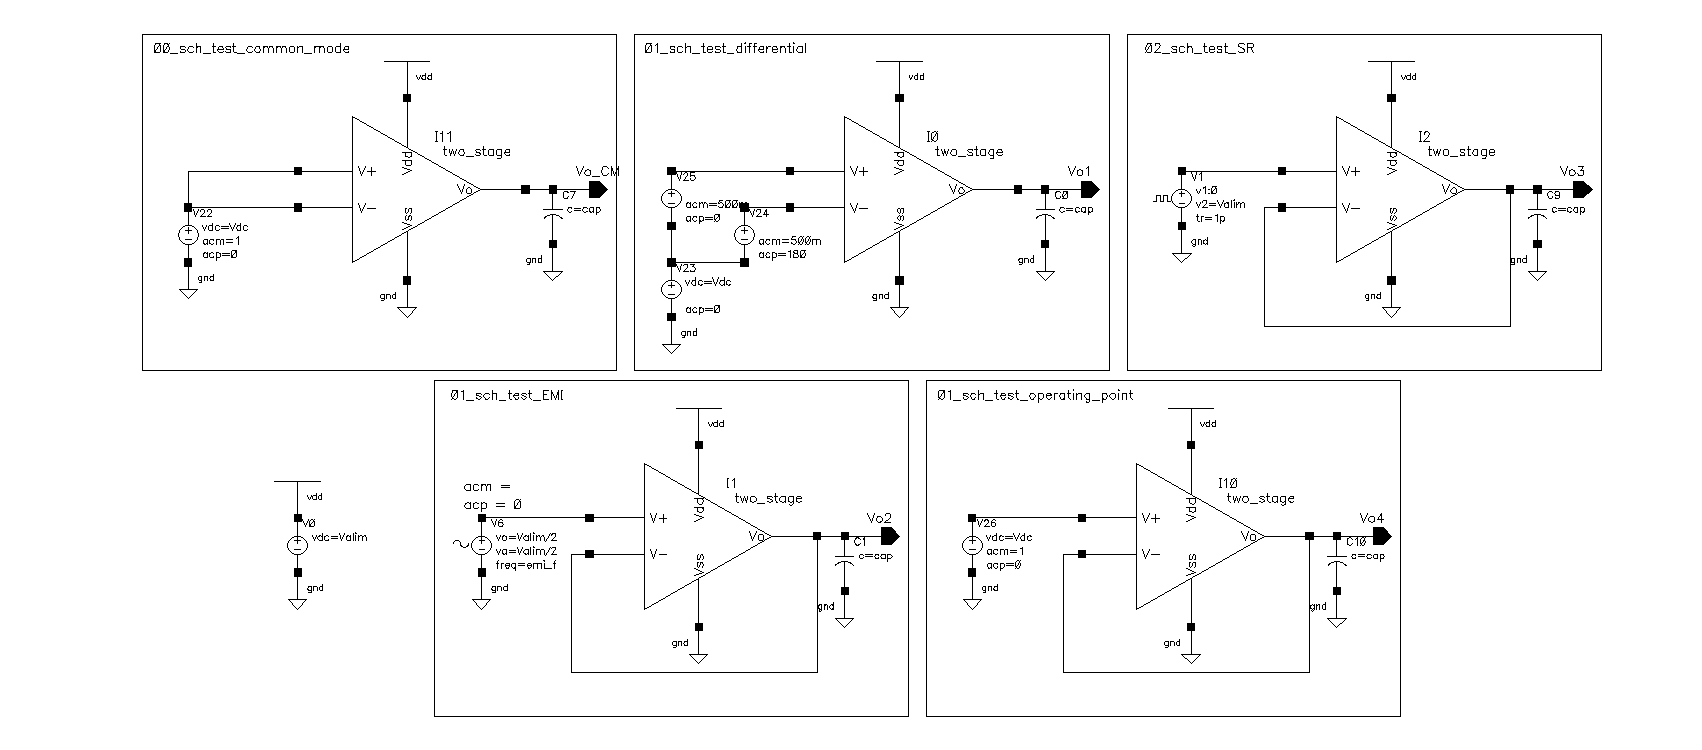
\includegraphics[width=\textwidth]{img/miller/double/sim_miller_double_stage.png}
    \caption{Schematico di riferimento per l'OTA di Miller a stadio doppio.}
    \label{fig:schematic_miller_double_stage}
\end{figure}

Il blocco \textit{two\_stage\_MillerOTA} dell'OTA di Miller a stadio doppio viene riportato nella figura \ref{fig:schematic_miller_double_stage_inverter}.

\begin{figure}[H]
    \centering
    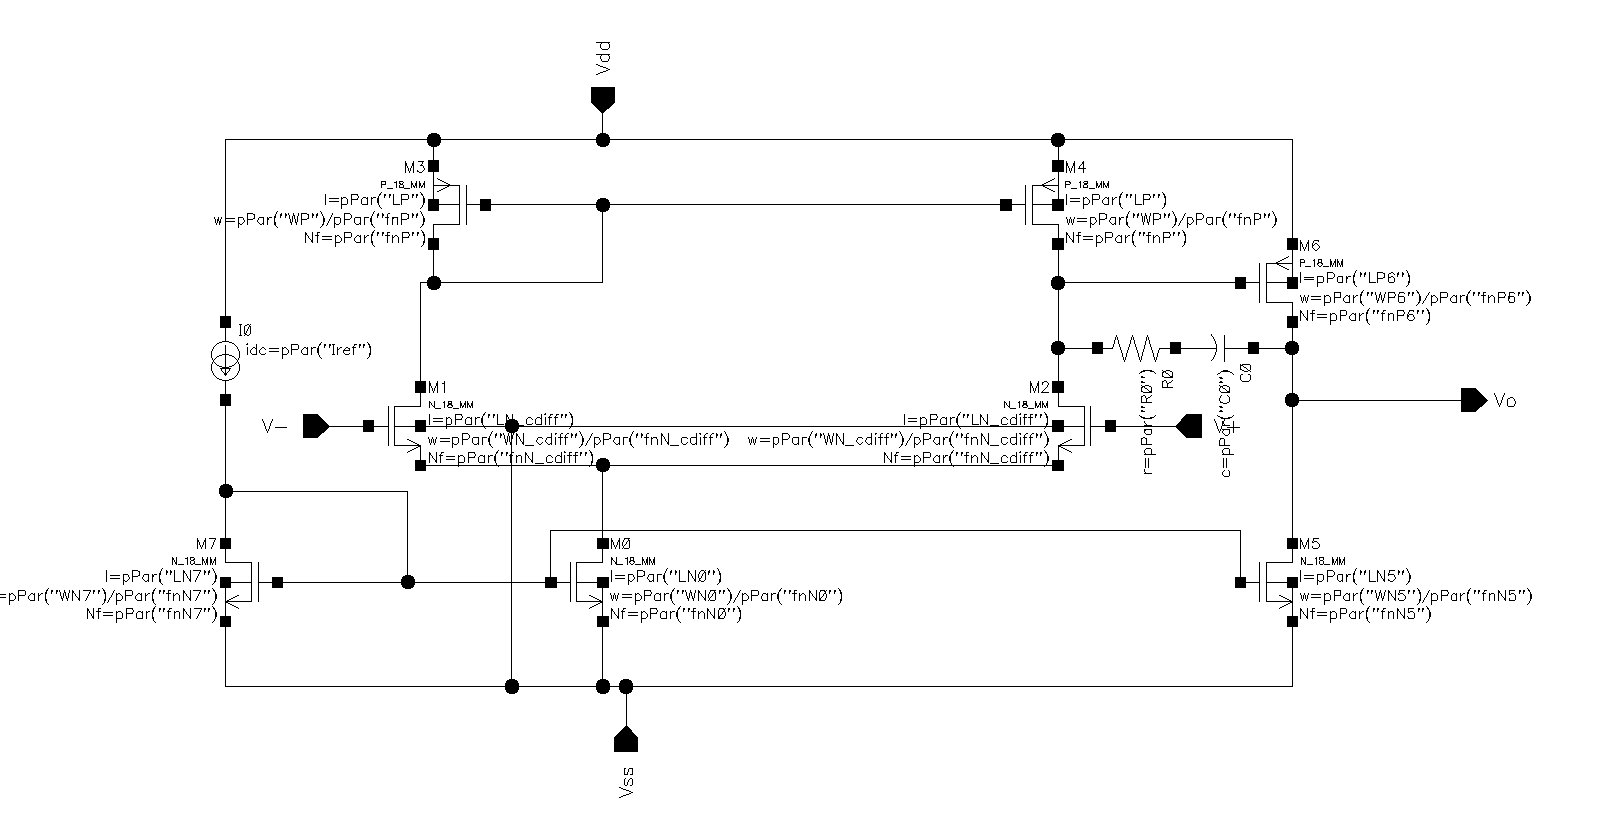
\includegraphics[width=\textwidth]{img/miller/double/sch_miller_double_stage.png}
    \caption{Schematico di riferimento per il blocco \textit{two\_stage\_MillerOTA} dell'OTA di Miller a stadio doppio.}
    \label{fig:schematic_miller_double_stage}
\end{figure}

\subsection{Dimensionamento dei componenti}
\label{sec:results_ota_miller_double_stage_component_sizing}
I parametri di dimensionamento sono stati scelti in modo da garantire un guadagno di tensione intorno a 40 dB e un margine di fase di almeno 60°. I valori di dimensionamento scelti e i relativi risultati sono riportati nella Tabella \ref{tab:component_sizing_miller_double_stage}.

\begin{longtable}{c|c|c|}
    \caption{Dimensionamento dei componenti dell'OTA di Miller a stadio doppio. Tutti i risultati sono stati ottenuti con una capacità di carico di 1pF.}
    \label{tab:component_sizing_miller_double_stage} \\
    
    \cline{2-3}
    & \textbf{Valim = 1V} & \textbf{Valim = 1.8V} \\ \hline
    \multicolumn{3}{|c|}{\textbf{Parametri di simulazione}} \\ \hline
    \endfirsthead
    
    \multicolumn{3}{c}{\tablename\ \thetable{} -- Continua dalla pagina precedente} \\
    \cline{2-3}
    & \textbf{Valim = 1V} & \textbf{Valim = 1.8V} \\ \hline
    \endhead
    
    \multicolumn{3}{r}{{Continua nella pagina successiva}} \\
    \endfoot
    
    \endlastfoot

    \multicolumn{1}{|c|}{C0} & 5pF & 5pF \\ \hline
    \multicolumn{1}{|c|}{Iref} & 20$\mu$A & 20$\mu$A \\ \hline
    \multicolumn{1}{|c|}{LN0} & 1$\mu$m & 1$\mu$m \\ \hline
    \multicolumn{1}{|c|}{LN5} & 1$\mu$m & 1$\mu$m \\ \hline
    \multicolumn{1}{|c|}{LN7} & 1$\mu$m & 1$\mu$m \\ \hline
    \multicolumn{1}{|c|}{LN\_cdiff} & 1$\mu$m & 1$\mu$m \\ \hline
    \multicolumn{1}{|c|}{LP} & 1$\mu$m & 1$\mu$m \\ \hline
    \multicolumn{1}{|c|}{LP6} & 1$\mu$m & 1$\mu$m \\ \hline
    \multicolumn{1}{|c|}{R0} & 5k$\Omega$ & 5k$\Omega$ \\ \hline
    \multicolumn{1}{|c|}{WN0} & 32$\mu$m & 32$\mu$m \\ \hline
    \multicolumn{1}{|c|}{WN5} & 28$\mu$m & 28$\mu$m \\ \hline
    \multicolumn{1}{|c|}{WN7} & 32$\mu$m & 32$\mu$m \\ \hline
    \multicolumn{1}{|c|}{WN\_cdiff} & 24$\mu$m & 24$\mu$m \\ \hline
    \multicolumn{1}{|c|}{WP} & 32$\mu$m & 32$\mu$m \\ \hline
    \multicolumn{1}{|c|}{WP6} & 72$\mu$m & 72$\mu$m \\ \hline
    \multicolumn{1}{|c|}{cap} & 1pF & 1pF \\ \hline
    \multicolumn{1}{|c|}{fnN0} & 8 & 8 \\ \hline
    \multicolumn{1}{|c|}{fnN5} & 8 & 8 \\ \hline
    \multicolumn{1}{|c|}{fnN7} & 8 & 8 \\ \hline
    \multicolumn{1}{|c|}{fnN\_cdiff} & 8 & 8 \\ \hline
    \multicolumn{1}{|c|}{fnP} & 8 & 8 \\ \hline
    \multicolumn{1}{|c|}{fnP6} & 36 & 36 \\ \hline
    \multicolumn{3}{|c|}{\textbf{Risultati simulazione}} \\ \hline
    \multicolumn{1}{|c|}{M0 region} & 2 & 2 \\ \hline
    \multicolumn{1}{|c|}{M1 region} & 2 & 2 \\ \hline
    \multicolumn{1}{|c|}{M2 region} & 2 & 2 \\ \hline
    \multicolumn{1}{|c|}{M3 region} & 2 & 2 \\ \hline
    \multicolumn{1}{|c|}{M4 region} & 2 & 2 \\ \hline
    \multicolumn{1}{|c|}{M5 region} & 2 & 2 \\ \hline
    \multicolumn{1}{|c|}{M6 region} & 2 & 2 \\ \hline
    \multicolumn{1}{|c|}{M7 region} & 2 & 2 \\ \hline
    \multicolumn{1}{|c|}{Ipol} & 17.25$\mu$A & 20.02$\mu$A \\ \hline
    \multicolumn{1}{|c|}{AV(0)} & 71.85dB & 72.16dB \\ \hline
    \multicolumn{1}{|c|}{f$_c$} & 1.421kHz & 1.573kHz \\ \hline
    \multicolumn{1}{|c|}{f$_o$} & 5.708MHz & 6.787MHz \\ \hline
\end{longtable}


\subsubsection{A$_v$, Phase, CMRR e CMR}
\label{sec:results_ota_miller_double_stage_A_V_phase}
Di seguito vengono riportati i risultati delle simulazioni per il guadagno di tensione ($A_V$) e la fase (Phase) dell'OTA di Miller a stadio doppio.

\begin{figure}[H]
    \centering
    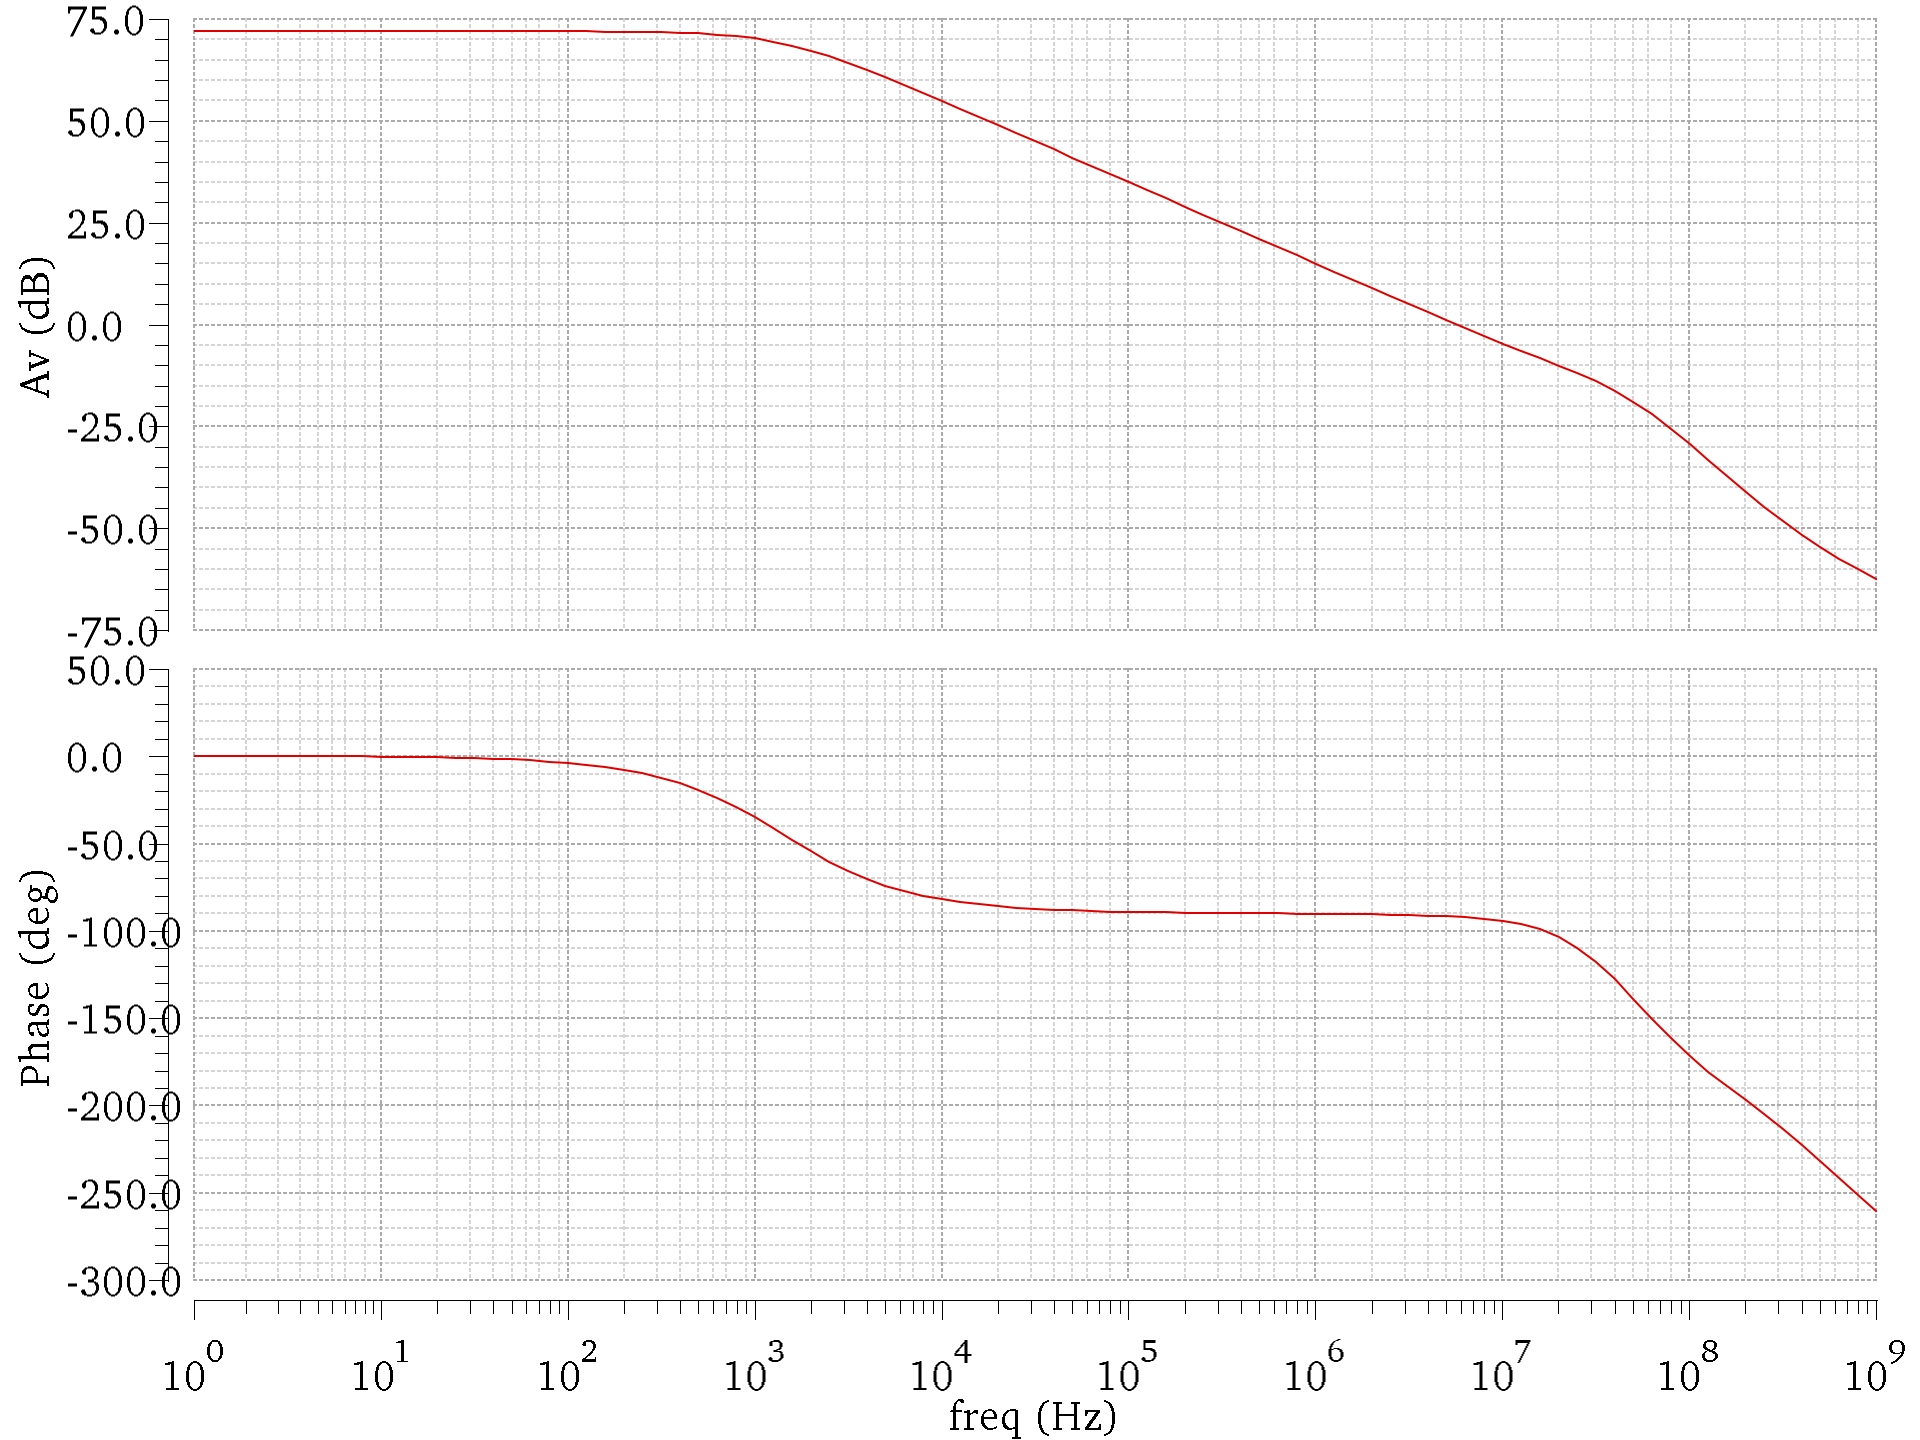
\includegraphics[width=\textwidth]{img/miller/double/av_ph_1V.jpg}
    \caption{Risultati delle simulazioni per il guadagno di tensione ($A_V$) e la fase (Phase) dell'OTA di Miller a stadio doppio con Valim = 1V.}
    \label{fig:results_miller_double_stage_A_V_phase_1V}
\end{figure}

\begin{figure}[H]
    \centering
    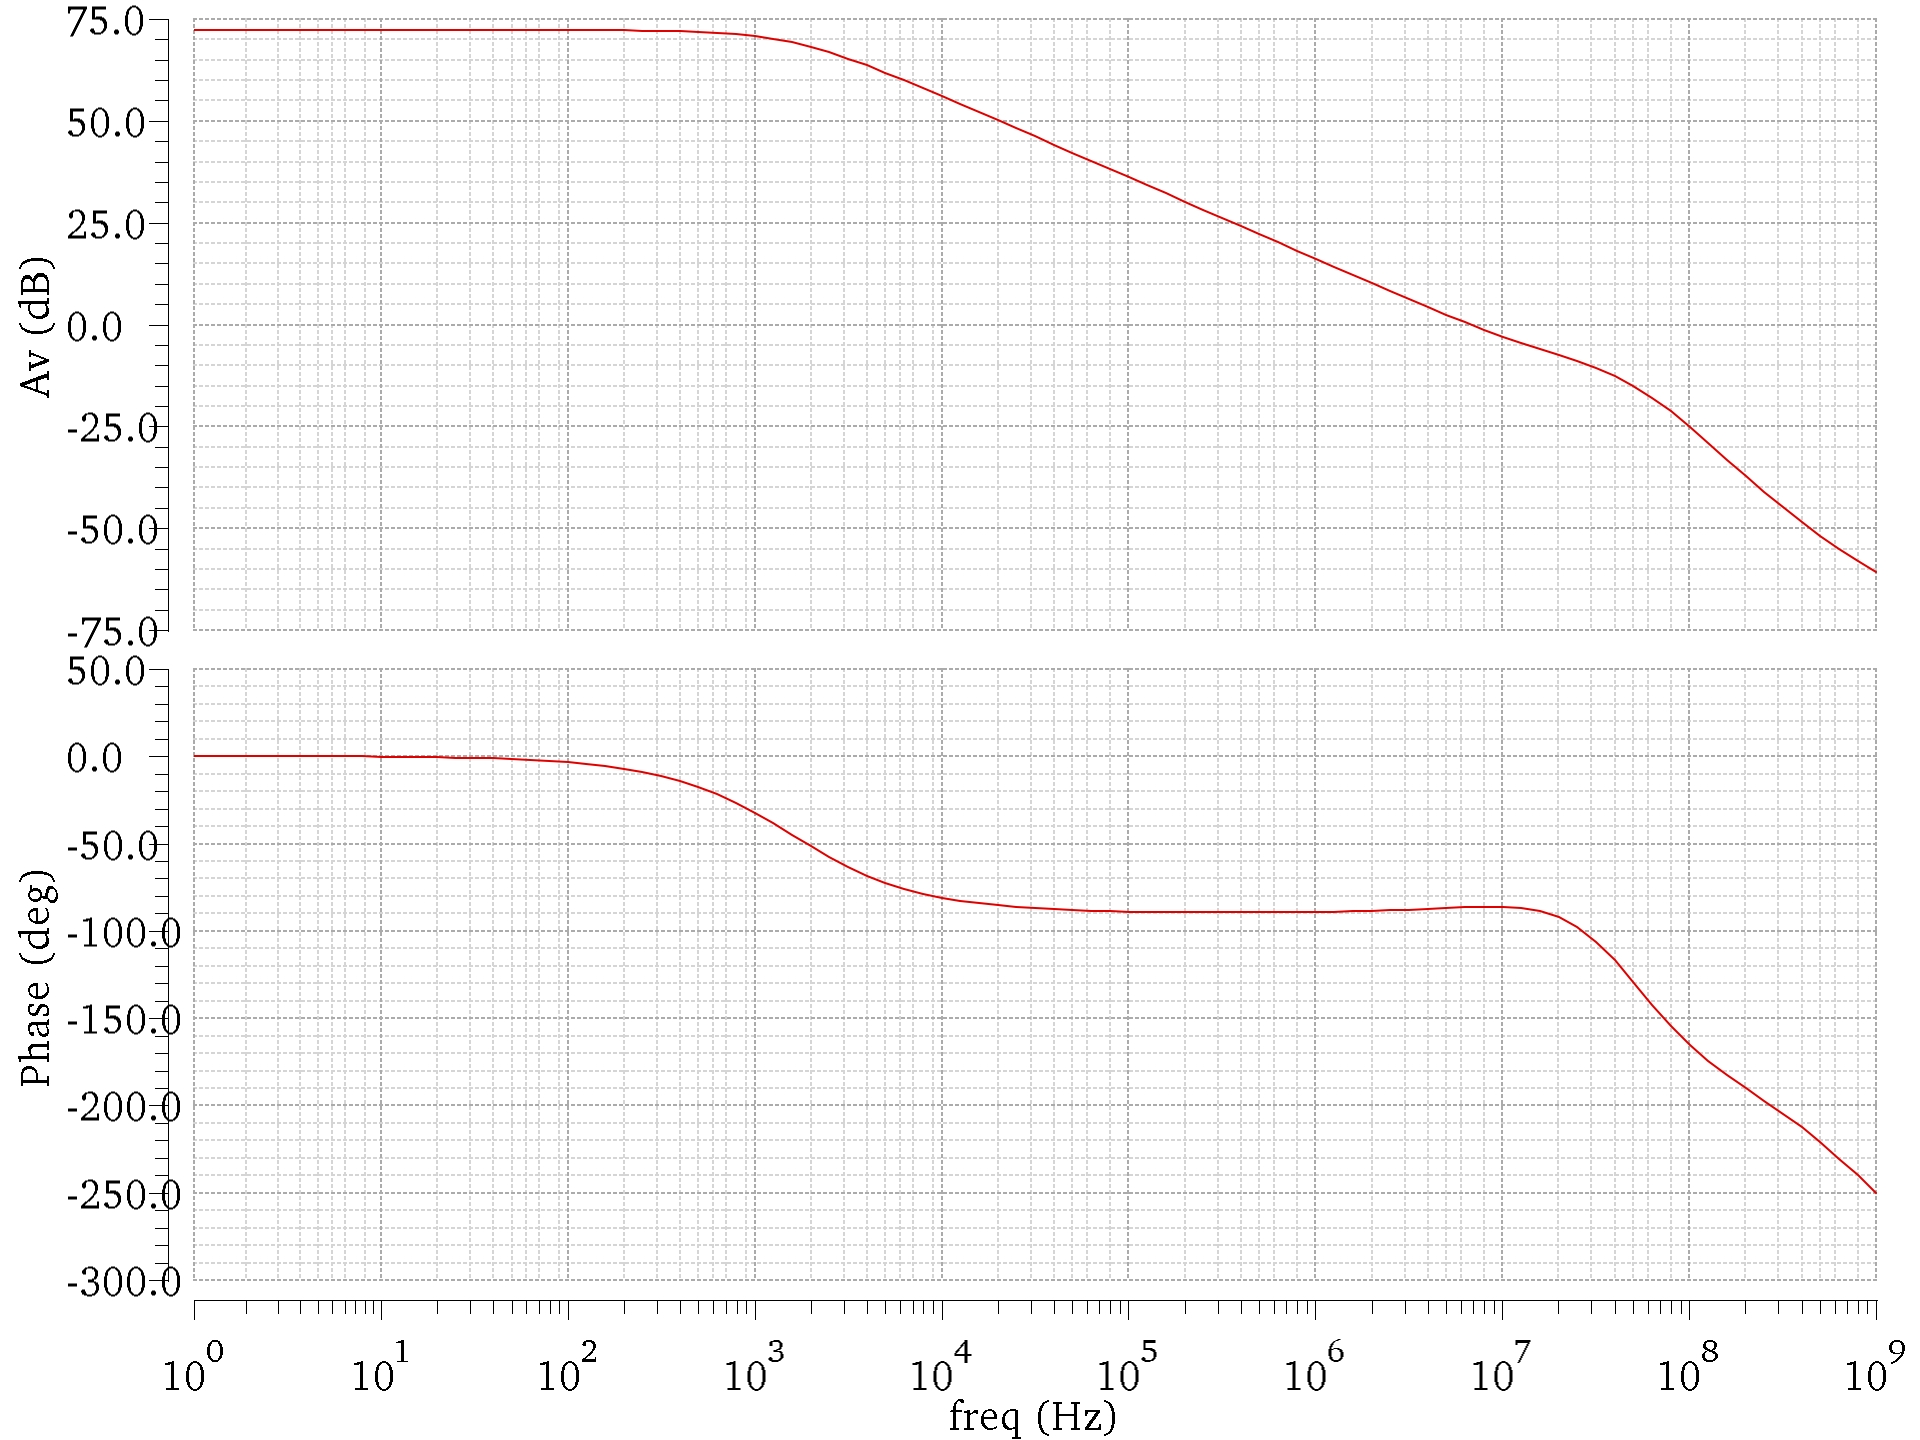
\includegraphics[width=\textwidth]{img/miller/double/av_ph_1_8V.jpg}
    \caption{Risultati delle simulazioni per il guadagno di tensione ($A_V$) e la fase (Phase) dell'OTA di Miller a stadio doppio con Valim = 1.8V.}
    \label{fig:results_miller_double_stage_A_V_phase_1_8V}
\end{figure}

Di seguito vengono riportati i risultati delle simulazioni per il rapporto di reiezione al modo comume (CMRR) e il range di modo comune (CMR) dell'OTA di Miller a stadio doppio.

\begin{figure}[H]
    \centering
    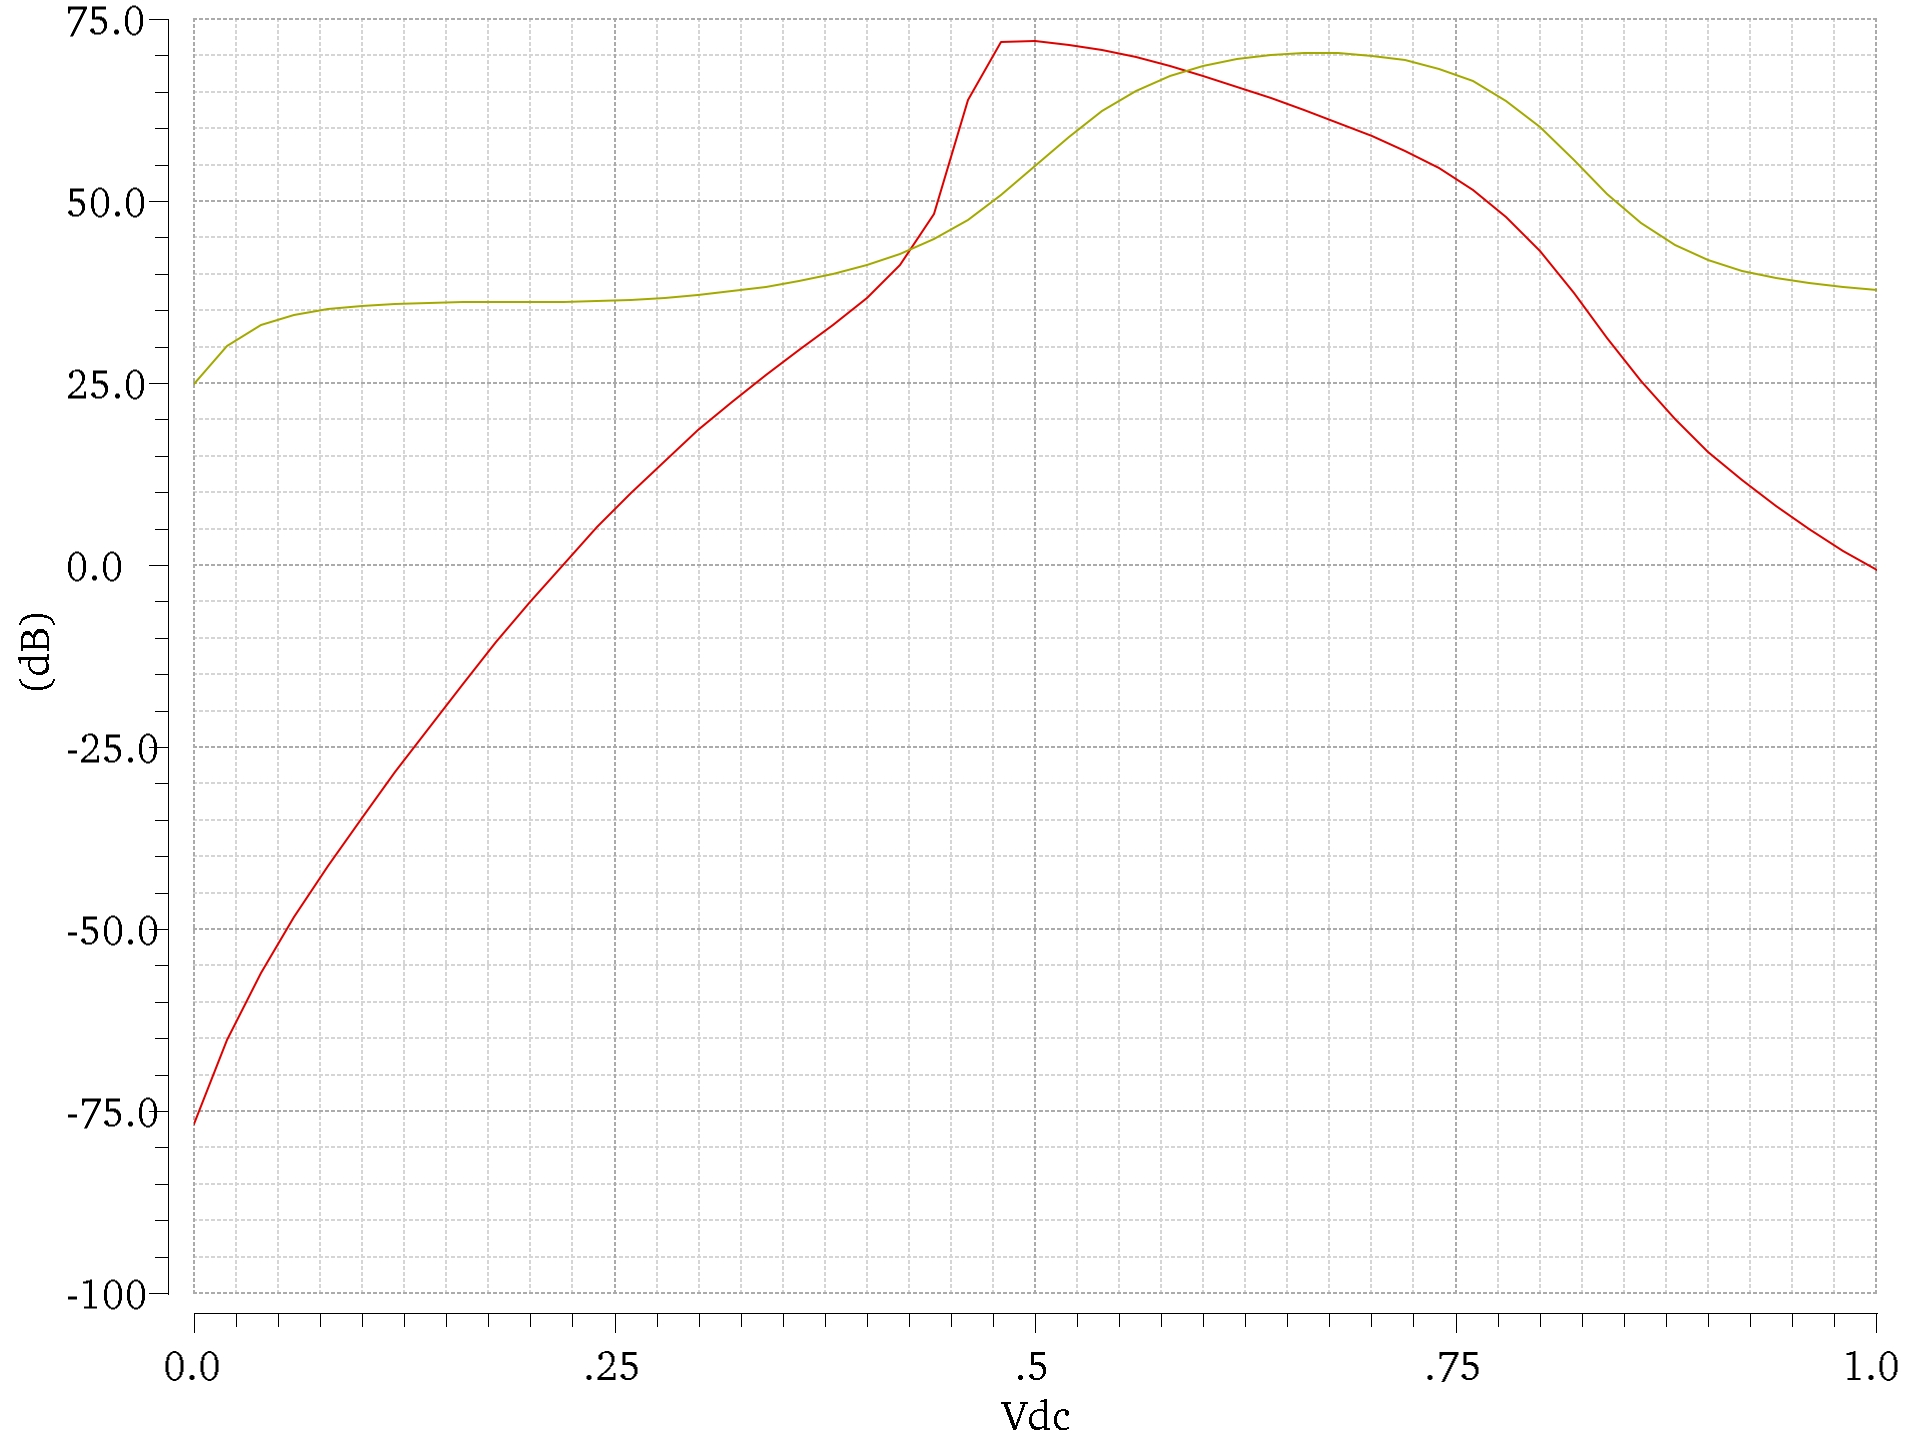
\includegraphics[width=\textwidth]{img/miller/double/cmr_cmrr_1V.jpg}
    \vspace{0.2cm}
    \small
    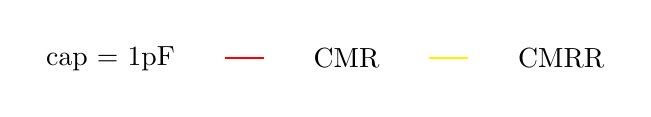
\begin{tikzpicture}
        \matrix[column sep=0.5cm, row sep=0.2cm] {
            \node[right]{cap = 1pF}; &
            \draw[red, thick] (0,0) -- (0.5,0); & \node{CMR}; &
            \draw[yellow, thick] (0,0) -- (0.5,0); & \node{CMRR}; \\
        };
    \end{tikzpicture}
    \caption{Risultati delle simulazioni per il rapporto di reiezione al modo comume (CMRR) e il range di modo comune (CMR) dell'OTA di Miller a stadio doppio con Valim = 1V.}
    \label{fig:results_miller_double_stage_CMRR_CMR_1V}
\end{figure}

Dai risultati delle simulazioni riportati nella figura \ref{fig:results_miller_double_stage_CMRR_CMR_1V} si osserva come il CMR sia peggiorato notevolmente rispetto alla configurazione a stadio singolo. Inoltre, alcuni range di tensione sono addirittura attenuati, il che significa che il circuito non è in grado di operare correttamente in quelle condizioni. 

\begin{figure}[H]
    \centering
    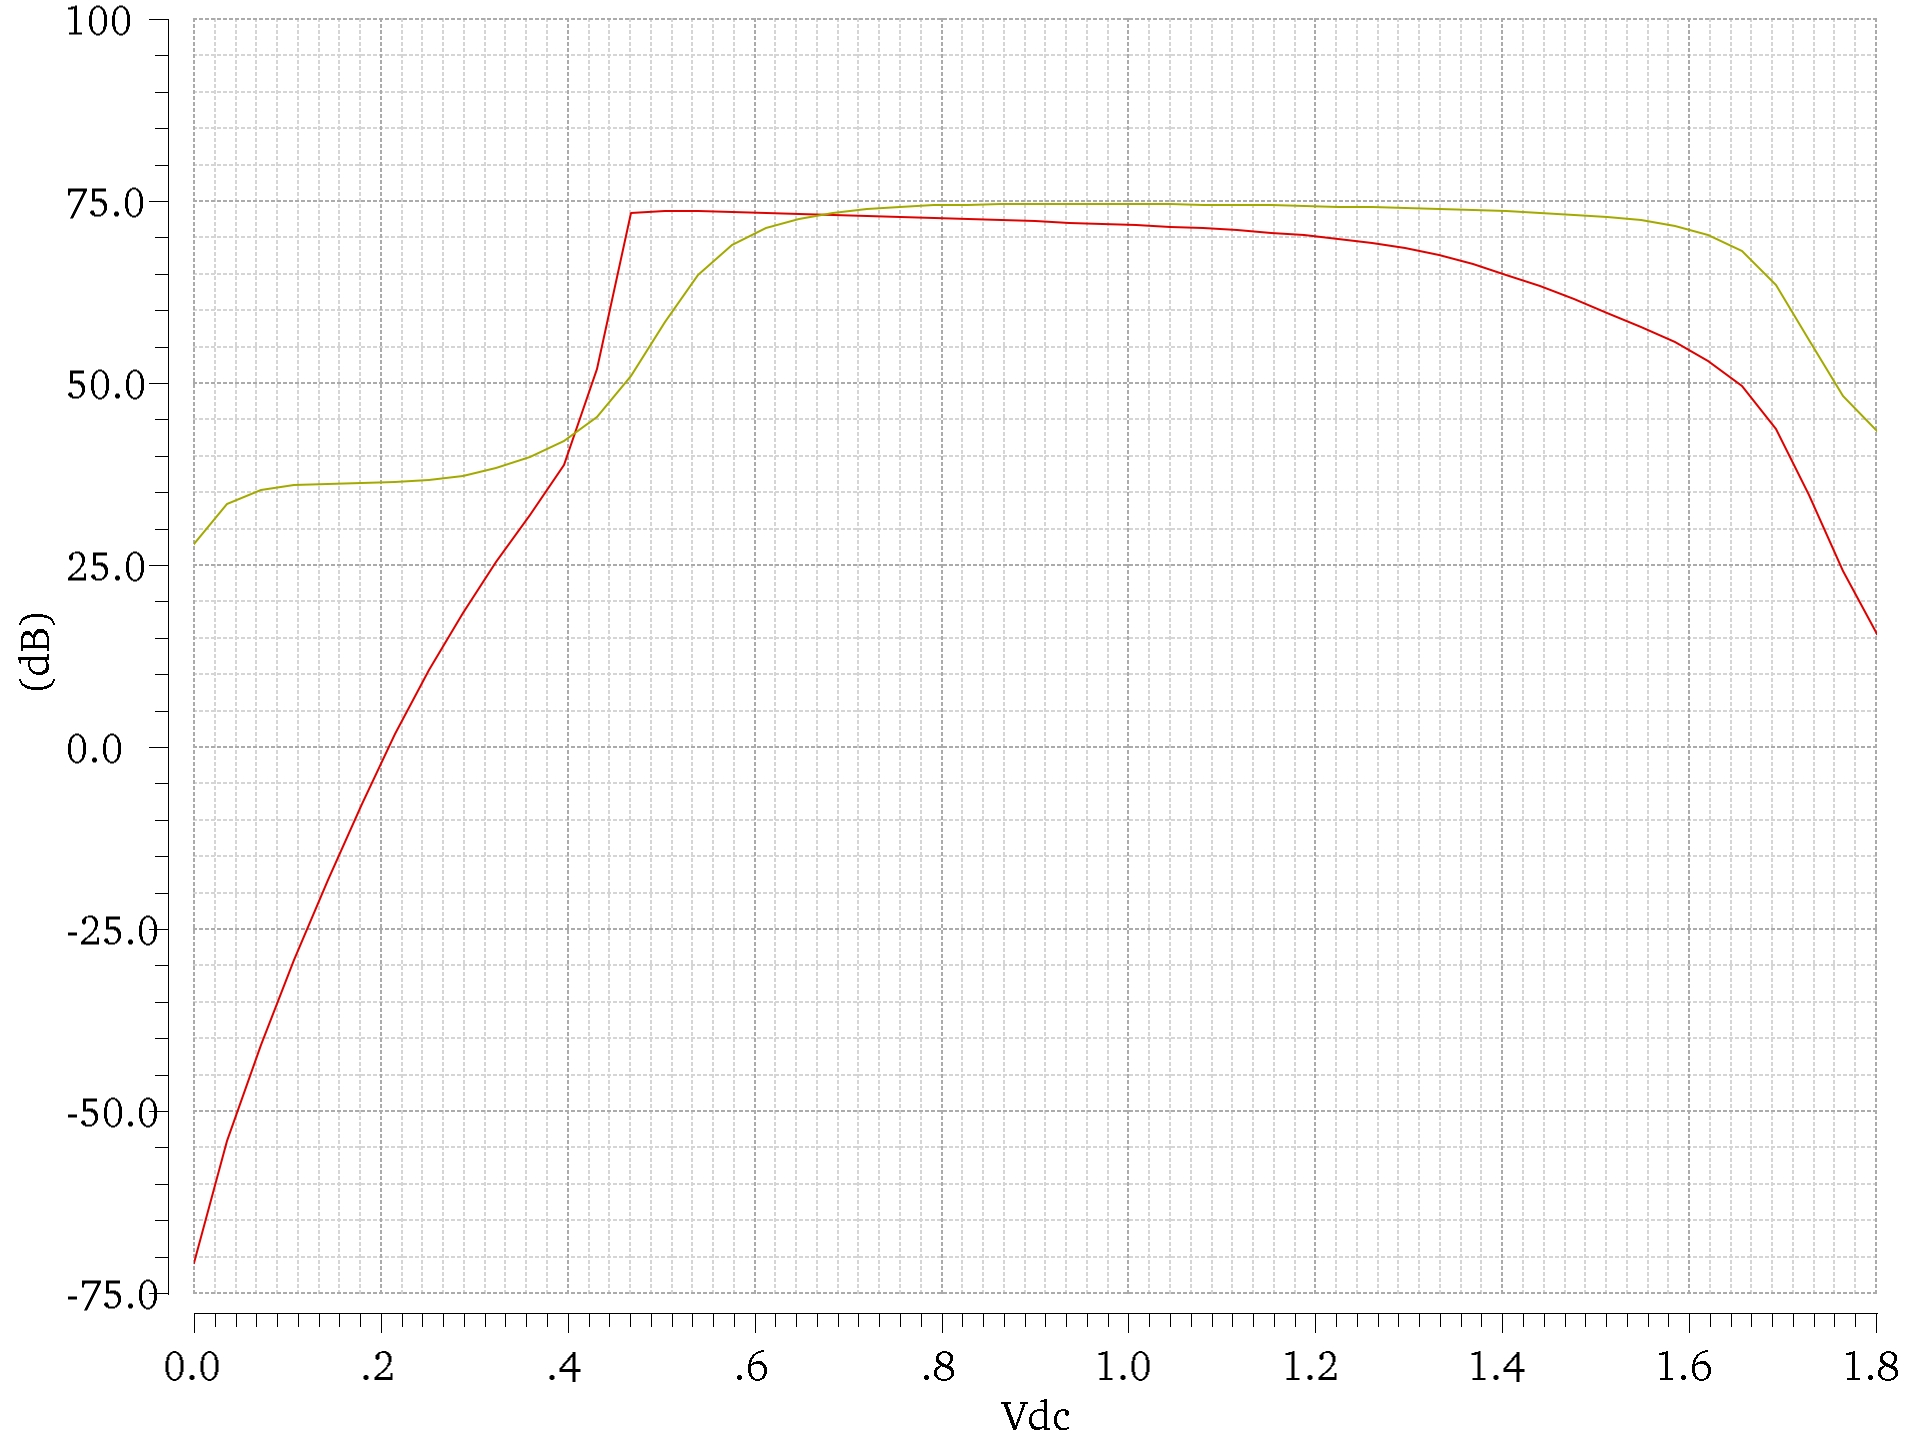
\includegraphics[width=\textwidth]{img/miller/double/cmr_cmrr_1_8V.jpg}
    \vspace{0.2cm}
    \small
    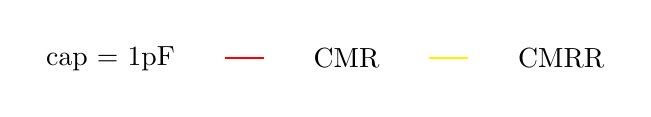
\begin{tikzpicture}
        \matrix[column sep=0.5cm, row sep=0.2cm] {
            \node[right]{cap = 1pF}; &
            \draw[red, thick] (0,0) -- (0.5,0); & \node{CMR}; &
            \draw[yellow, thick] (0,0) -- (0.5,0); & \node{CMRR}; \\
        };
    \end{tikzpicture}
    \caption{Risultati delle simulazioni per il rapporto di reiezione al modo comume (CMRR) e il range di modo comune (CMR) dell'OTA di Miller a stadio doppio con Valim = 1.8V.}
    \label{fig:results_miller_double_stage_CMRR_CMR_1_8V}
\end{figure}

Dai risultati delle simulazioni riportati nella figura \ref{fig:results_miller_double_stage_CMRR_CMR_1_8V} si osserva come il CMR sia anche in questo caso peggiorato rispetto alla configurazione a stadio singolo mostrata in figura \ref{fig:results_miller_single_stage_CMRR_CMR_1_8V}. Tuttavia si nota un miglioramento rispetto alla configurazione con Valim = 1V mostrata in figura \ref{fig:results_miller_double_stage_CMRR_CMR_1V}. 


\subsubsection{Phase Margin, Gain Bandwidth Product e Slew Rate}
\label{sec:results_ota_miller_double_stage_phase_margin_gain_bandwidth_product_slew_rate}

Di seguito vengono riportati i risultati delle simulazioni per il margine di fase (Phase Margin), il prodotto guadagno-banda (Gain Bandwidth Product) e lo slew rate (SR).

\begin{table}[H]
    \centering
    \caption{Risultati delle simulazioni per il margine di fase (Phase Margin), il prodotto guadagno-banda (Gain Bandwidth Product) e lo slew rate (SR) dell'OTA di Miller a doppio stadio con capacità di carico di 1pF.}
    \begin{tabular}{|c|c|c|c|}
        \hline
        \textbf{Valim} & \textbf{Phase Margin} & \textbf{Gain Bandwidth Product} & \textbf{Slew Rate (+/-)} \\ \hline
        1V & 88.03° & 5.6 MHz & 3.74/3.74 V/$\mu$s \\ \hline
        1.8V & 93.45° & 6.4 MHz & 4.53/4.53 V/$\mu$s \\ \hline
    \end{tabular}
    \label{tab:results_miller_double_stage_1pF}
\end{table}

\begin{table}[H]
    \centering
    \caption{Risultati delle simulazioni per il margine di fase (Phase Margin), il prodotto guadagno-banda (Gain Bandwidth Product) e lo slew rate (SR) dell'OTA di Miller a doppio stadio con capacità di carico di 10pF.}
    \begin{tabular}{|c|c|c|c|}
        \hline
        \textbf{Valim} & \textbf{Phase Margin} & \textbf{Gain Bandwidth Product} & \textbf{Slew Rate (+/-)} \\ \hline
        1V & 50.66° & 5.5 MHz & 3.53/3.53 V/$\mu$s \\ \hline
        1.8V & 53.94° & 6.3 MHz & 4.48/4.48 V/$\mu$s \\ \hline
    \end{tabular}
    \label{tab:results_miller_double_stage_10pF}
\end{table}



\subsubsection{Emi rejection}
\label{sec:results_ota_miller_double_stage_emi_rejection}
Di seguito vengono riportati i risultati delle simulazioni per l'emi rejection dell'OTA di Miller a stadio doppio. I risultati sono stati ottenuti con una capacità di carico di 1pF.

\begin{figure}[H]
    \centering
    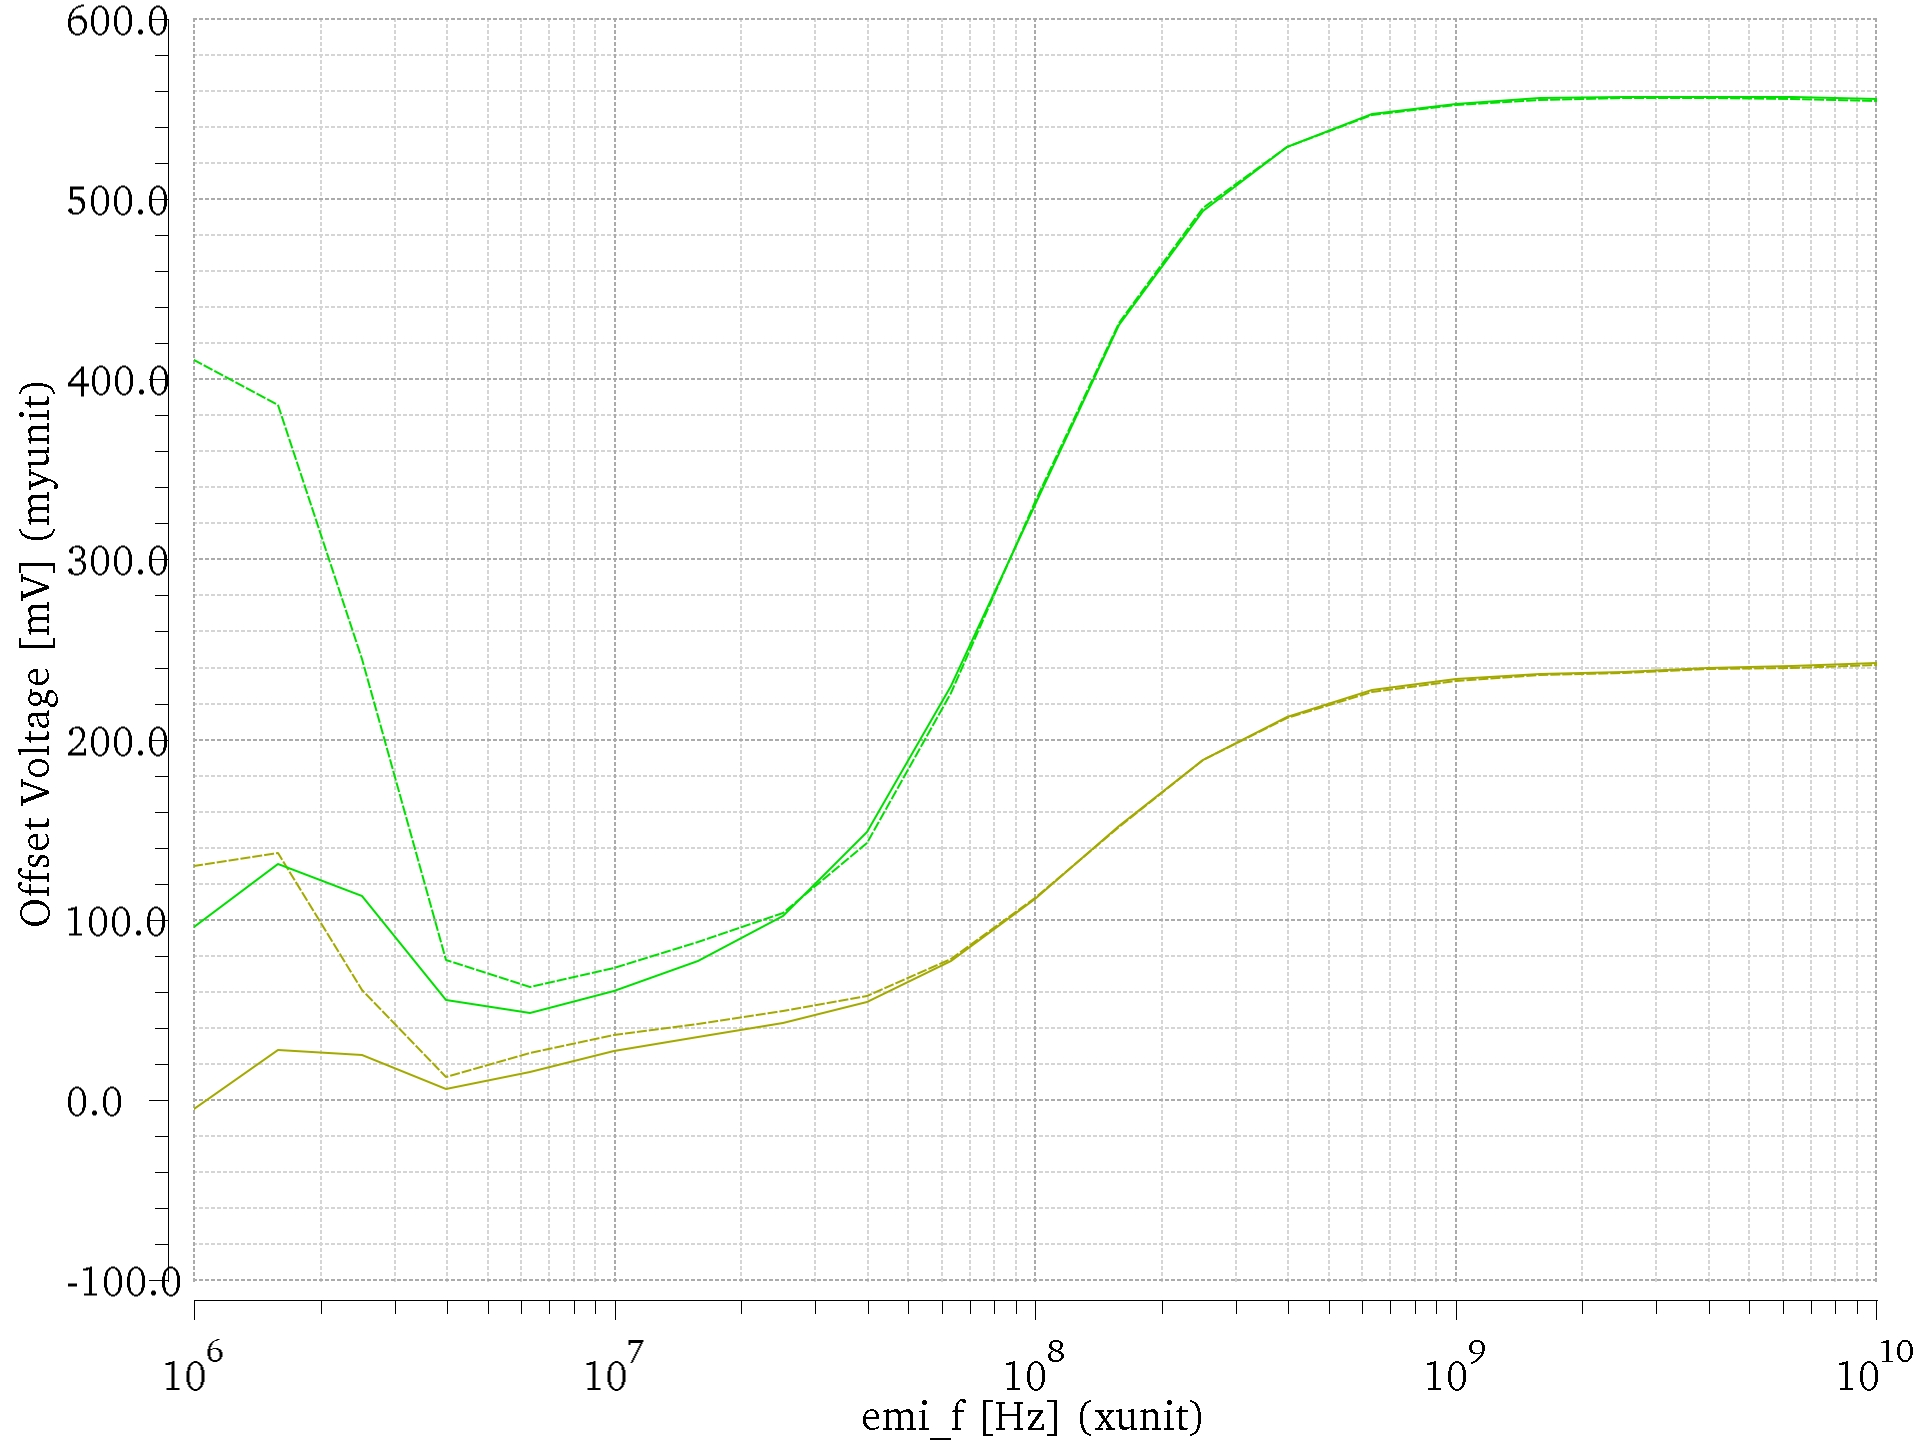
\includegraphics[width=\textwidth]{img/miller/double/emi_comparison.jpg}
    \vspace{0.2cm}
    \small
    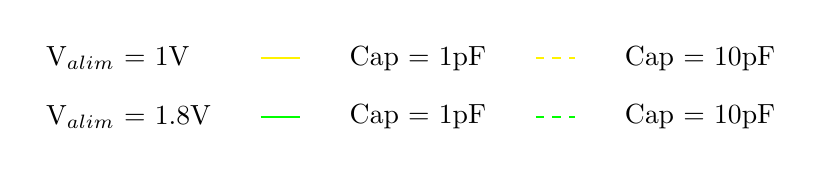
\begin{tikzpicture}
        \matrix[column sep=0.5cm, row sep=0.2cm] {
            \node[right]{V$_{alim}$ = 1V}; &
            \draw[yellow, thick] (0,0) -- (0.5,0); & \node{Cap = 1pF}; &
            \draw[yellow, thick, dashed] (0,0) -- (0.5,0); & \node{Cap = 10pF}; \\
            \node[right]{V$_{alim}$ = 1.8V}; &
            \draw[green, thick] (0,0) -- (0.5,0); & \node{Cap = 1pF}; &
            \draw[green, thick, dashed] (0,0) -- (0.5,0); & \node{Cap = 10pF}; \\
        };
    \end{tikzpicture}
    \caption{Risultati delle simulazioni per l'emi rejection dell'OTA di Miller a stadio doppio.}
    \label{fig:results_miller_double_stage_emi_rejection}
\end{figure}

\section{Sensibilità alle EMI a confronto tra i due OTA}
\label{sec:results_emi_comparison}

In questa sezione vengono confrontati i risultati delle simulazioni per l'emi rejection dell'OTA di Nauta e dell'OTA di Miller. I risultati sono stati ottenuti confrontando le simulazioni per i due OTA con una tensione di alimentazione di 1V e di 1.8V, e con una capacità di carico di 1pF e di 10pF. Il risultato mostra l'offset ottenuto sul segnale di output in funzione della frequenza del segnale di disturbo in ingresso.

\subsubsection{OTA a stadio singolo}
\label{sec:results_emi_comparison_single_stage}

\begin{figure}[H]
    \centering
    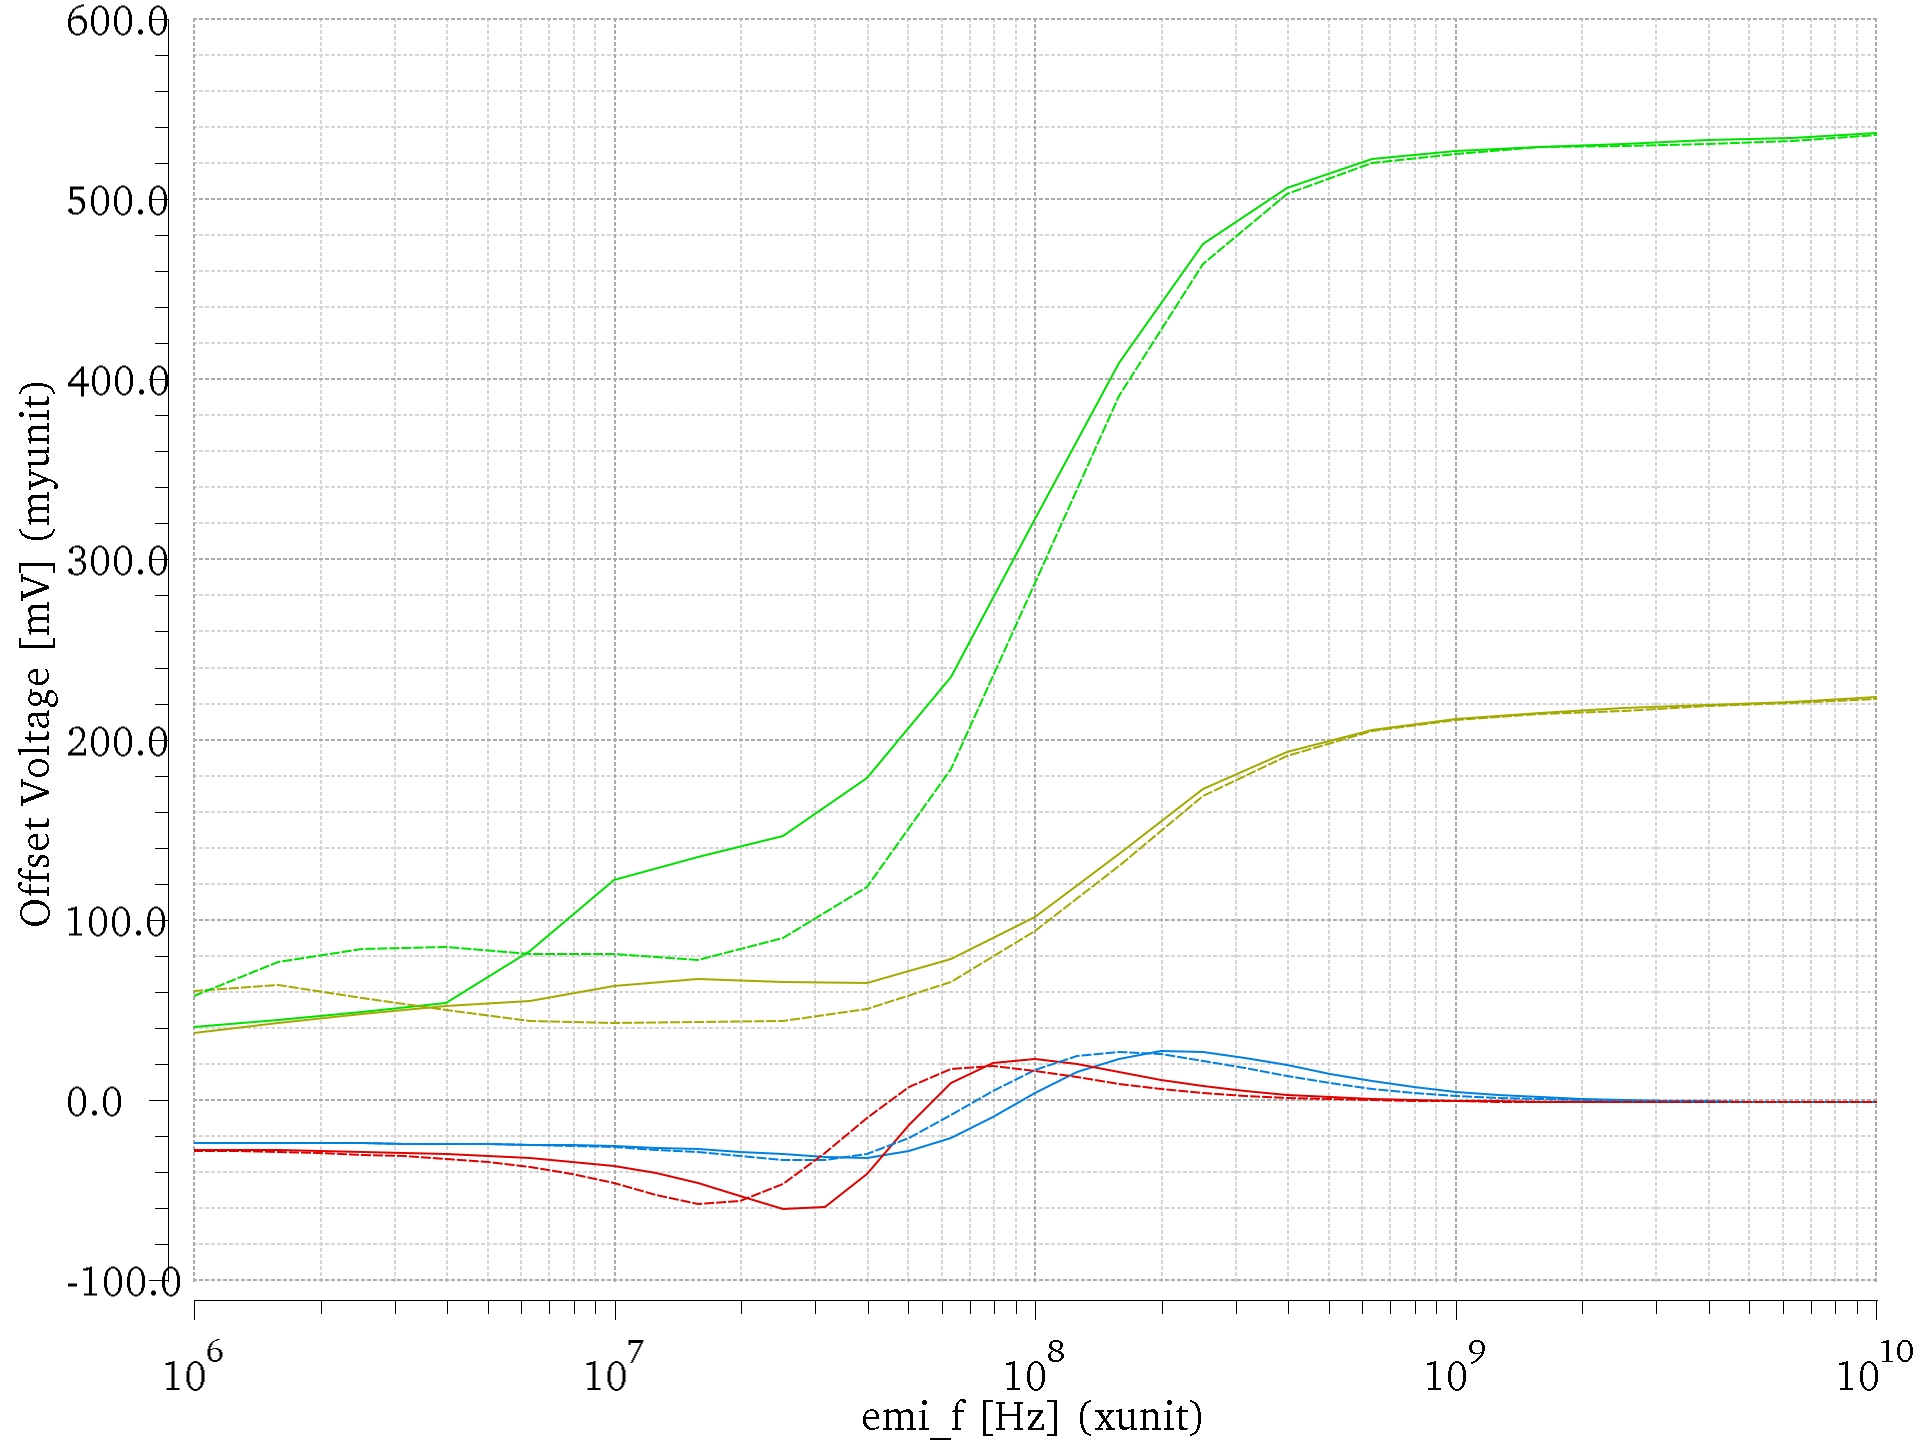
\includegraphics[width=\textwidth]{img/emi/emi_comparison_miller_nauta_single_stage.jpg}
    \vspace{0.2cm}
    \small
    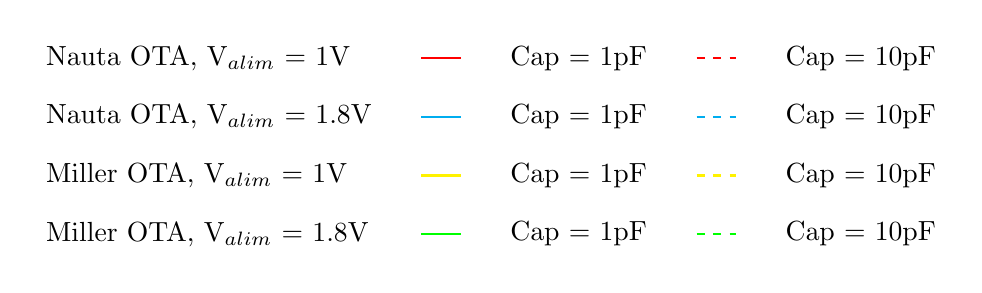
\begin{tikzpicture}
        \matrix[column sep=0.5cm, row sep=0.2cm] {
            \node[right]{Nauta OTA, V$_{alim}$ = 1V}; &
            \draw[red, thick] (0,0) -- (0.5,0); & \node{Cap = 1pF}; &
            \draw[red, thick, dashed] (0,0) -- (0.5,0); & \node{Cap = 10pF}; \\
            \node[right]{Nauta OTA, V$_{alim}$ = 1.8V}; &
            \draw[cyan, thick] (0,0) -- (0.5,0); & \node{Cap = 1pF}; &
            \draw[cyan, thick, dashed] (0,0) -- (0.5,0); & \node{Cap = 10pF}; \\
            \node[right]{Miller OTA, V$_{alim}$ = 1V}; &
            \draw[yellow, thick] (0,0) -- (0.5,0); & \node{Cap = 1pF}; &
            \draw[yellow, thick, dashed] (0,0) -- (0.5,0); & \node{Cap = 10pF}; \\
            \node[right]{Miller OTA, V$_{alim}$ = 1.8V}; &
            \draw[green, thick] (0,0) -- (0.5,0); & \node{Cap = 1pF}; &
            \draw[green, thick, dashed] (0,0) -- (0.5,0); & \node{Cap = 10pF}; \\
        };
    \end{tikzpicture}
    \caption{Risultati delle simulazioni per l'emi rejection dell'OTA di Nauta e dell'OTA di Miller a stadio singolo.}
    \label{fig:results_emi_comparison_single_stage}
\end{figure}

Il confronto tra i risultati delle simulazioni per l'emi rejection dell'OTA di Nauta e dell'OTA di Miller a stadio singolo mostrato nella figura \ref{fig:results_emi_comparison_single_stage} evidenzia che l'OTA di Nauta presenta una reiezione alle EMI migliore rispetto all'OTA di Miller. Questo è particolarmente evidente per entrambe le tensioni di alimentazione, inoltre, entrambi gli OTA mostrano una risposta poco sensibile alla capacità di carico. È importante sottolineare come per frequenze superiori al GHz, l'OTA di Nauta presenta un'offset nullo sul segnale di output rendendo quindi il circuito immune alle EMI. 

\subsubsection{OTA a stadio doppio}
\label{sec:results_emi_comparison_double_stage}

\begin{figure}[H]
    \centering
    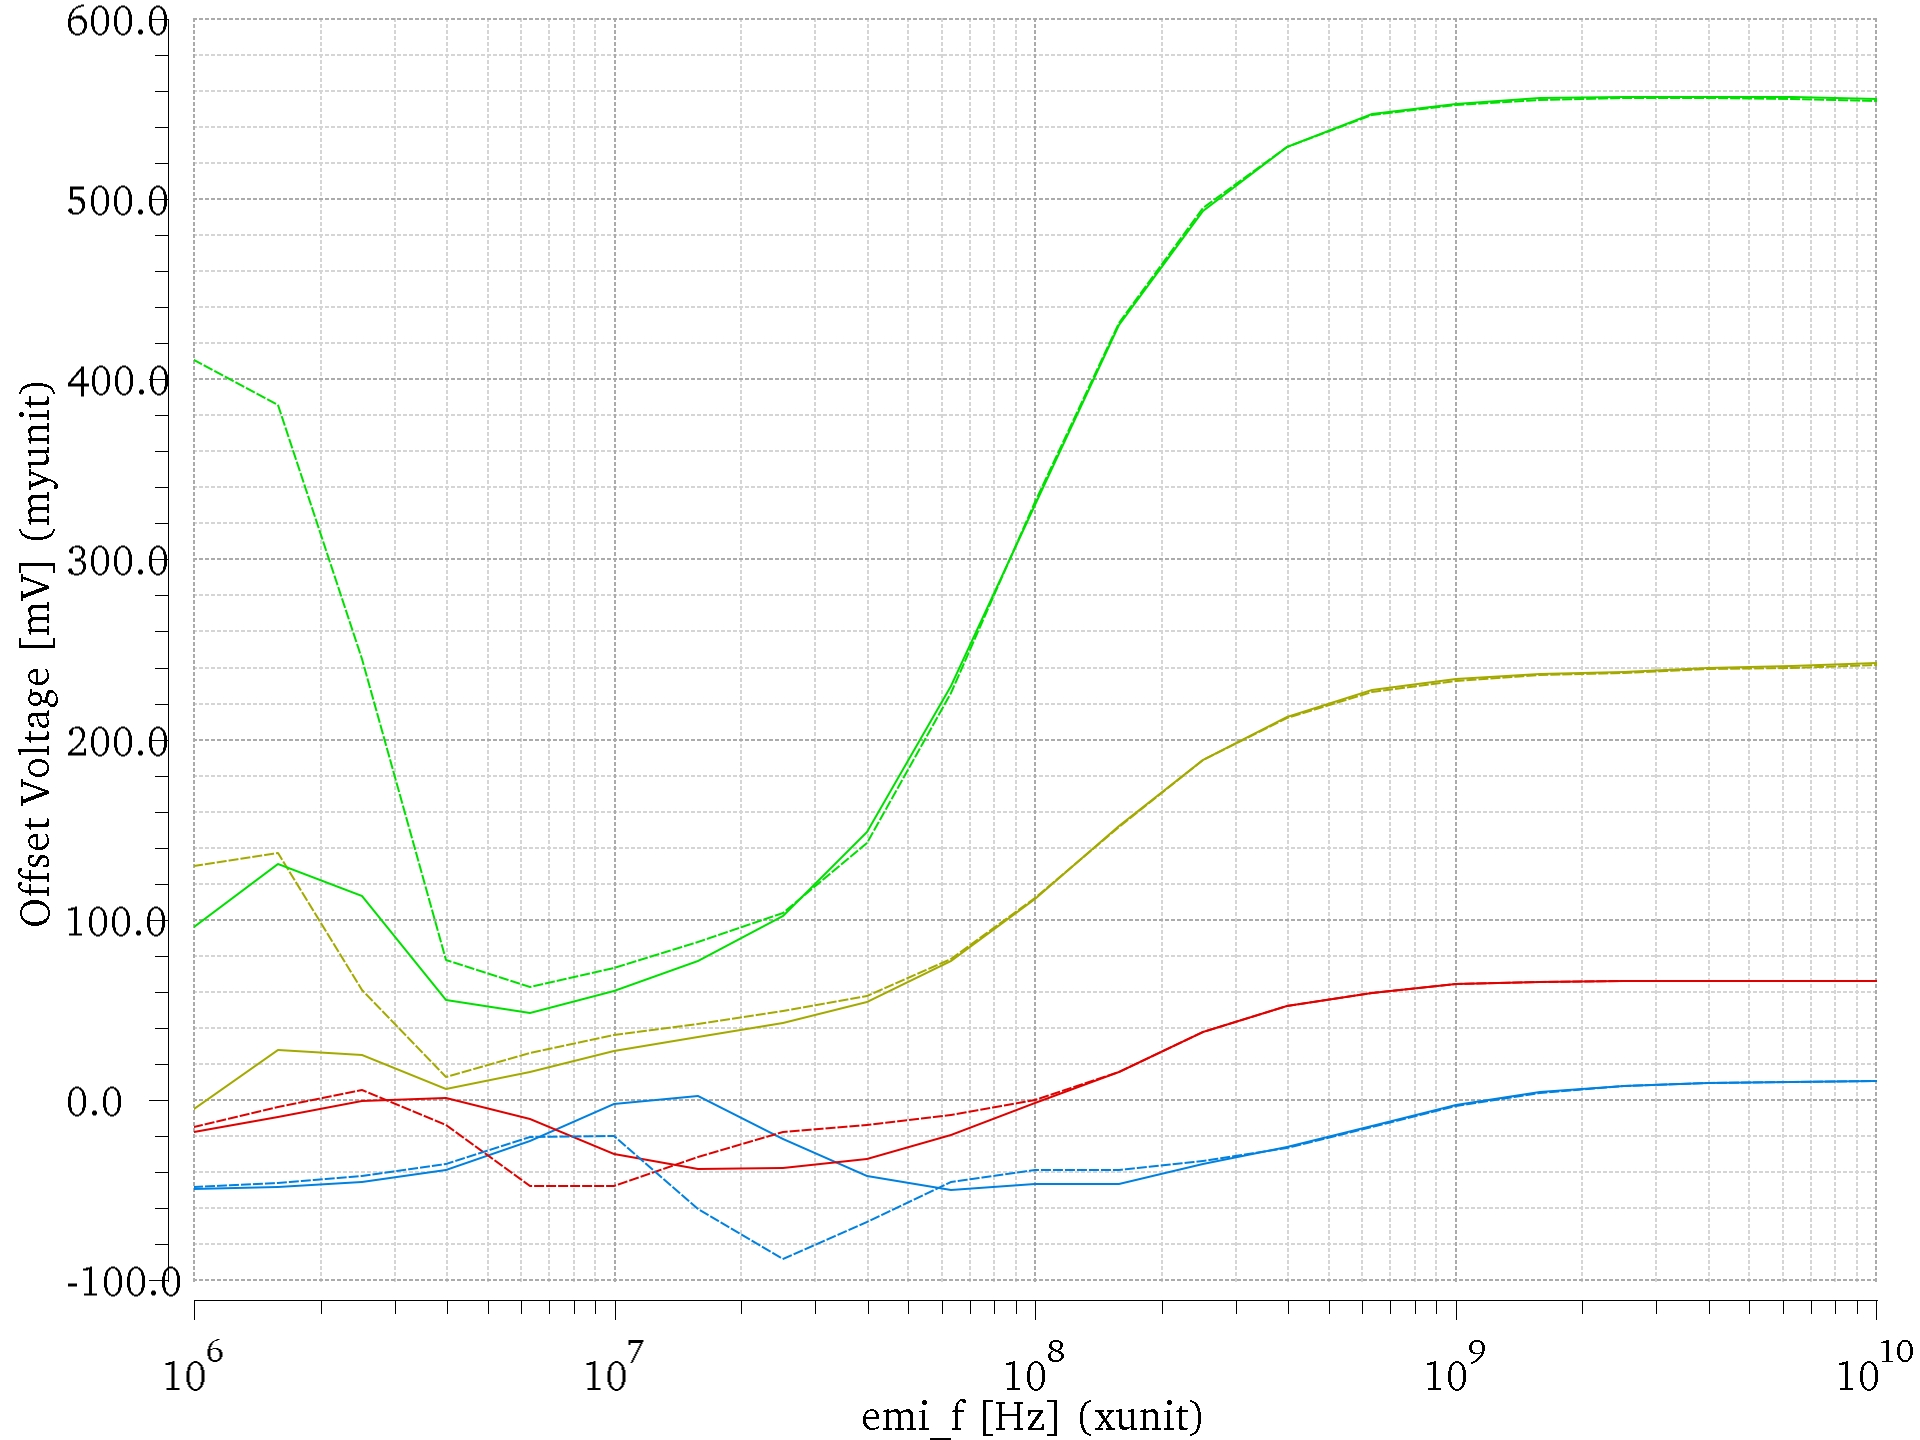
\includegraphics[width=\textwidth]{img/emi/emi_comparison_miller_nauta_two_staged.jpg}
    \vspace{0.2cm}
    \small
    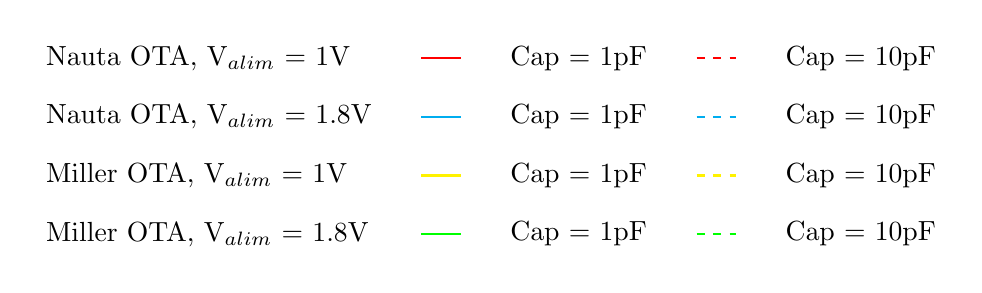
\begin{tikzpicture}
        \matrix[column sep=0.5cm, row sep=0.2cm] {
            \node[right]{Nauta OTA, V$_{alim}$ = 1V}; &
            \draw[red, thick] (0,0) -- (0.5,0); & \node{Cap = 1pF}; &
            \draw[red, thick, dashed] (0,0) -- (0.5,0); & \node{Cap = 10pF}; \\
            \node[right]{Nauta OTA, V$_{alim}$ = 1.8V}; &
            \draw[cyan, thick] (0,0) -- (0.5,0); & \node{Cap = 1pF}; &
            \draw[cyan, thick, dashed] (0,0) -- (0.5,0); & \node{Cap = 10pF}; \\
            \node[right]{Miller OTA, V$_{alim}$ = 1V}; &
            \draw[yellow, thick] (0,0) -- (0.5,0); & \node{Cap = 1pF}; &
            \draw[yellow, thick, dashed] (0,0) -- (0.5,0); & \node{Cap = 10pF}; \\
            \node[right]{Miller OTA, V$_{alim}$ = 1.8V}; &
            \draw[green, thick] (0,0) -- (0.5,0); & \node{Cap = 1pF}; &
            \draw[green, thick, dashed] (0,0) -- (0.5,0); & \node{Cap = 10pF}; \\
        };
    \end{tikzpicture}
    \caption{Risultati delle simulazioni per l'emi rejection dell'OTA di Nauta e dell'OTA di Miller a stadio doppio.}
    \label{fig:results_emi_comparison_double_stage}
\end{figure}

Il confronto tra i risultati delle simulazioni per l'emi rejection dell'OTA di Nauta e dell'OTA di Miller a stadio doppio mostrato nella figura \ref{fig:results_emi_comparison_double_stage} evidenzia che anche in questo caso l'OTA di Nauta presenta una reiezione alle EMI migliore rispetto all'OTA di Miller. Tuttavia, a differenza dell'OTA a stadio singolo, l'OTA di Nauta mostra una risposta più sensibile alla tensione di alimentazione riportando un'offset di qualche decina di mV sul segnale di output per basse tensioni. Infatti, se si osserva la figura \ref{fig:results_nauta_double_stage_emi_rejection} è possibile notare come l'immunità alle EMI diminuisca notevolmente per tensioni di alimentazione decrescenti.
